% Options for packages loaded elsewhere
\PassOptionsToPackage{unicode}{hyperref}
\PassOptionsToPackage{hyphens}{url}
%
\documentclass[
]{book}
\usepackage{amsmath,amssymb}
\usepackage{lmodern}
\usepackage{iftex}
\ifPDFTeX
  \usepackage[T1]{fontenc}
  \usepackage[utf8]{inputenc}
  \usepackage{textcomp} % provide euro and other symbols
\else % if luatex or xetex
  \usepackage{unicode-math}
  \defaultfontfeatures{Scale=MatchLowercase}
  \defaultfontfeatures[\rmfamily]{Ligatures=TeX,Scale=1}
\fi
% Use upquote if available, for straight quotes in verbatim environments
\IfFileExists{upquote.sty}{\usepackage{upquote}}{}
\IfFileExists{microtype.sty}{% use microtype if available
  \usepackage[]{microtype}
  \UseMicrotypeSet[protrusion]{basicmath} % disable protrusion for tt fonts
}{}
\makeatletter
\@ifundefined{KOMAClassName}{% if non-KOMA class
  \IfFileExists{parskip.sty}{%
    \usepackage{parskip}
  }{% else
    \setlength{\parindent}{0pt}
    \setlength{\parskip}{6pt plus 2pt minus 1pt}}
}{% if KOMA class
  \KOMAoptions{parskip=half}}
\makeatother
\usepackage{xcolor}
\usepackage{color}
\usepackage{fancyvrb}
\newcommand{\VerbBar}{|}
\newcommand{\VERB}{\Verb[commandchars=\\\{\}]}
\DefineVerbatimEnvironment{Highlighting}{Verbatim}{commandchars=\\\{\}}
% Add ',fontsize=\small' for more characters per line
\usepackage{framed}
\definecolor{shadecolor}{RGB}{248,248,248}
\newenvironment{Shaded}{\begin{snugshade}}{\end{snugshade}}
\newcommand{\AlertTok}[1]{\textcolor[rgb]{0.94,0.16,0.16}{#1}}
\newcommand{\AnnotationTok}[1]{\textcolor[rgb]{0.56,0.35,0.01}{\textbf{\textit{#1}}}}
\newcommand{\AttributeTok}[1]{\textcolor[rgb]{0.77,0.63,0.00}{#1}}
\newcommand{\BaseNTok}[1]{\textcolor[rgb]{0.00,0.00,0.81}{#1}}
\newcommand{\BuiltInTok}[1]{#1}
\newcommand{\CharTok}[1]{\textcolor[rgb]{0.31,0.60,0.02}{#1}}
\newcommand{\CommentTok}[1]{\textcolor[rgb]{0.56,0.35,0.01}{\textit{#1}}}
\newcommand{\CommentVarTok}[1]{\textcolor[rgb]{0.56,0.35,0.01}{\textbf{\textit{#1}}}}
\newcommand{\ConstantTok}[1]{\textcolor[rgb]{0.00,0.00,0.00}{#1}}
\newcommand{\ControlFlowTok}[1]{\textcolor[rgb]{0.13,0.29,0.53}{\textbf{#1}}}
\newcommand{\DataTypeTok}[1]{\textcolor[rgb]{0.13,0.29,0.53}{#1}}
\newcommand{\DecValTok}[1]{\textcolor[rgb]{0.00,0.00,0.81}{#1}}
\newcommand{\DocumentationTok}[1]{\textcolor[rgb]{0.56,0.35,0.01}{\textbf{\textit{#1}}}}
\newcommand{\ErrorTok}[1]{\textcolor[rgb]{0.64,0.00,0.00}{\textbf{#1}}}
\newcommand{\ExtensionTok}[1]{#1}
\newcommand{\FloatTok}[1]{\textcolor[rgb]{0.00,0.00,0.81}{#1}}
\newcommand{\FunctionTok}[1]{\textcolor[rgb]{0.00,0.00,0.00}{#1}}
\newcommand{\ImportTok}[1]{#1}
\newcommand{\InformationTok}[1]{\textcolor[rgb]{0.56,0.35,0.01}{\textbf{\textit{#1}}}}
\newcommand{\KeywordTok}[1]{\textcolor[rgb]{0.13,0.29,0.53}{\textbf{#1}}}
\newcommand{\NormalTok}[1]{#1}
\newcommand{\OperatorTok}[1]{\textcolor[rgb]{0.81,0.36,0.00}{\textbf{#1}}}
\newcommand{\OtherTok}[1]{\textcolor[rgb]{0.56,0.35,0.01}{#1}}
\newcommand{\PreprocessorTok}[1]{\textcolor[rgb]{0.56,0.35,0.01}{\textit{#1}}}
\newcommand{\RegionMarkerTok}[1]{#1}
\newcommand{\SpecialCharTok}[1]{\textcolor[rgb]{0.00,0.00,0.00}{#1}}
\newcommand{\SpecialStringTok}[1]{\textcolor[rgb]{0.31,0.60,0.02}{#1}}
\newcommand{\StringTok}[1]{\textcolor[rgb]{0.31,0.60,0.02}{#1}}
\newcommand{\VariableTok}[1]{\textcolor[rgb]{0.00,0.00,0.00}{#1}}
\newcommand{\VerbatimStringTok}[1]{\textcolor[rgb]{0.31,0.60,0.02}{#1}}
\newcommand{\WarningTok}[1]{\textcolor[rgb]{0.56,0.35,0.01}{\textbf{\textit{#1}}}}
\usepackage{longtable,booktabs,array}
\usepackage{calc} % for calculating minipage widths
% Correct order of tables after \paragraph or \subparagraph
\usepackage{etoolbox}
\makeatletter
\patchcmd\longtable{\par}{\if@noskipsec\mbox{}\fi\par}{}{}
\makeatother
% Allow footnotes in longtable head/foot
\IfFileExists{footnotehyper.sty}{\usepackage{footnotehyper}}{\usepackage{footnote}}
\makesavenoteenv{longtable}
\usepackage{graphicx}
\makeatletter
\def\maxwidth{\ifdim\Gin@nat@width>\linewidth\linewidth\else\Gin@nat@width\fi}
\def\maxheight{\ifdim\Gin@nat@height>\textheight\textheight\else\Gin@nat@height\fi}
\makeatother
% Scale images if necessary, so that they will not overflow the page
% margins by default, and it is still possible to overwrite the defaults
% using explicit options in \includegraphics[width, height, ...]{}
\setkeys{Gin}{width=\maxwidth,height=\maxheight,keepaspectratio}
% Set default figure placement to htbp
\makeatletter
\def\fps@figure{htbp}
\makeatother
\setlength{\emergencystretch}{3em} % prevent overfull lines
\providecommand{\tightlist}{%
  \setlength{\itemsep}{0pt}\setlength{\parskip}{0pt}}
\setcounter{secnumdepth}{5}
\usepackage{booktabs}
\usepackage{amsthm}
\makeatletter
\def\thm@space@setup{%
  \thm@preskip=8pt plus 2pt minus 4pt
  \thm@postskip=\thm@preskip
}
\makeatother
\ifLuaTeX
  \usepackage{selnolig}  % disable illegal ligatures
\fi
\usepackage[]{natbib}
\bibliographystyle{apalike}
\IfFileExists{bookmark.sty}{\usepackage{bookmark}}{\usepackage{hyperref}}
\IfFileExists{xurl.sty}{\usepackage{xurl}}{} % add URL line breaks if available
\urlstyle{same} % disable monospaced font for URLs
\hypersetup{
  pdftitle={Advanced Econometrics},
  pdfauthor={Jean-Paul Renne},
  hidelinks,
  pdfcreator={LaTeX via pandoc}}

\title{Advanced Econometrics}
\author{Jean-Paul Renne}
\date{2022-09-16}

\usepackage{amsthm}
\newtheorem{theorem}{Theorem}[chapter]
\newtheorem{lemma}{Lemma}[chapter]
\newtheorem{corollary}{Corollary}[chapter]
\newtheorem{proposition}{Proposition}[chapter]
\newtheorem{conjecture}{Conjecture}[chapter]
\theoremstyle{definition}
\newtheorem{definition}{Definition}[chapter]
\theoremstyle{definition}
\newtheorem{example}{Example}[chapter]
\theoremstyle{definition}
\newtheorem{exercise}{Exercise}[chapter]
\theoremstyle{definition}
\newtheorem{hypothesis}{Hypothesis}[chapter]
\theoremstyle{remark}
\newtheorem*{remark}{Remark}
\newtheorem*{solution}{Solution}
\begin{document}
\maketitle

{
\setcounter{tocdepth}{1}
\tableofcontents
}
\newcommand{\bv}[1]{\mathbf{#1}}

\hypertarget{intro}{%
\chapter{Before starting}\label{intro}}

This course covers various econometric topics, including linear regression models, discrete-choice models, and time series analysis. It provides examples or simulations based on R codes.

The R codes use various packages that can be obtained from \href{https://cran.r-project.org}{CRAN}. Several pieces of code also involve procedures and data from my \texttt{AEC} package. The latter is available on GitHub. To install it, one need to employ the \texttt{devtools} library:

\begin{Shaded}
\begin{Highlighting}[]
\FunctionTok{library}\NormalTok{(devtools)}
\FunctionTok{install\_github}\NormalTok{(}\StringTok{"jrenne/AEC"}\NormalTok{)}
\FunctionTok{library}\NormalTok{(AEC)}
\end{Highlighting}
\end{Shaded}

\textbf{Useful (R) links:}

\begin{itemize}
\item
  Download R:

  \begin{itemize}
  \tightlist
  \item
    R software: \url{https://cran.r-project.org} (the basic R software)
  \item
    RStudio: \url{https://www.rstudio.com} (a convenient R editor)
  \end{itemize}
\item
  Tutorials:

  \begin{itemize}
  \tightlist
  \item
    Rstudio: \url{https://dss.princeton.edu/training/RStudio101.pdf} (by Oscar Torres-Reyna)
  \item
    R: \url{https://cran.r-project.org/doc/contrib/Paradis-rdebuts_en.pdf} (by Emmanuel Paradis)
  \item
    My own tutorial: \url{https://jrenne.shinyapps.io/Rtuto_publiShiny/}
  \end{itemize}
\end{itemize}

\hypertarget{TS}{%
\chapter{Time Series}\label{TS}}

\hypertarget{VAR}{%
\section{Multivariate models}\label{VAR}}

This section presents Vector Auto-Regressive Moving-Average (SVARMA) models. These models are widely used in macroeconomic analysis. While simple and easy to estimate, they make it possible to conveniently capture the dynamics of complex multivariate systems. VAR popularity is notably due to \citet{Sims_1980}'s influential work. A nice survey if proposed by \citet{Stock_Watson_2016}.

In economics, VAR models are often employed in order to identify \emph{structural} shocks, that are independent primitive exogenous forces that drive economic variables (\citet{Ramey_2016_NBER}). They are often given a specific economic meaning (e.g., demand and supply shocks).

Working with these models (VAR and VARMA models) often is often based on two steps: in a first step, the \textbf{reduced-form} version of the model is estimated; in a second step, structural shocks are identified and IRFs are produced.

\citet{Kilian_1998} See \href{https://rdrr.io/cran/VAR.etp/man/VAR.Boot.html}{this page}

Sign restrictions: \href{https://github.com/chrstdanne/VARsignR}{package}, \citet{Danne_2015}.

\citet{vars}

\citet{bvartools}: R package to estimate Bayesian VAR models.

\begin{Shaded}
\begin{Highlighting}[]
\FunctionTok{library}\NormalTok{(VAR.etp)}
\FunctionTok{library}\NormalTok{(vars) }\CommentTok{\#standard VAR models}
\FunctionTok{data}\NormalTok{(dat) }\CommentTok{\# part of VAR.etp package}
\NormalTok{a }\OtherTok{\textless{}{-}} \FunctionTok{VAR.Boot}\NormalTok{(dat,}\AttributeTok{p=}\DecValTok{2}\NormalTok{,}\AttributeTok{nb=}\DecValTok{200}\NormalTok{,}\AttributeTok{type=}\StringTok{"const"}\NormalTok{)}
\NormalTok{b }\OtherTok{\textless{}{-}} \FunctionTok{VAR}\NormalTok{(dat,}\AttributeTok{p=}\DecValTok{2}\NormalTok{)}
\FunctionTok{rbind}\NormalTok{(a}\SpecialCharTok{$}\NormalTok{coef[}\DecValTok{1}\NormalTok{,],(a}\SpecialCharTok{$}\NormalTok{coef}\SpecialCharTok{+}\NormalTok{a}\SpecialCharTok{$}\NormalTok{Bias)[}\DecValTok{1}\NormalTok{,],b}\SpecialCharTok{$}\NormalTok{varresult}\SpecialCharTok{$}\NormalTok{inv}\SpecialCharTok{$}\NormalTok{coefficients)}
\end{Highlighting}
\end{Shaded}

\begin{verbatim}
##         inv(-1)   inc(-1)   con(-1)    inv(-2)   inc(-2)   con(-2)       const
## [1,] -0.3146496 0.2087952 0.9400172 -0.1499038 0.1253967 0.9521322 -0.01837906
## [2,] -0.3196310 0.1459888 0.9612190 -0.1605511 0.1146050 0.9343938 -0.01672199
## [3,] -0.3196310 0.1459888 0.9612190 -0.1605511 0.1146050 0.9343938 -0.01672199
\end{verbatim}

\hypertarget{definition-of-vars-and-svarma-models}{%
\subsection{Definition of VARs (and SVARMA) models}\label{definition-of-vars-and-svarma-models}}

\begin{definition}[(S)VAR model]
\protect\hypertarget{def:SVAR}{}\label{def:SVAR}Let \(y_{t}\) denote a \(n \times1\) vector of random variables. Process \(y_{t}\) follows a \(p^{th}\)-order VAR if, for all \(t\), we have
\begin{eqnarray}
\begin{array}{rllll}
VAR:& y_t &=& c + \Phi_1 y_{t-1} + \dots + \Phi_p y_{t-p} + \varepsilon_t,\\
SVAR:& y_t &=& c + \Phi_1 y_{t-1} + \dots + \Phi_p y_{t-p} + B \eta_t,
\end{array}\label{eq:yVAR}
\end{eqnarray}
with \(\varepsilon_t = B\eta_t\). We assume that \(\{\eta_{t}\}\) is a white noise sequence whose components are are mutually and serially independent.
\end{definition}

The first line of Eq. \eqref{eq:yVAR} corresponds to the \textbf{reduced-form} of the VAR model (\textbf{structural form} for the second line).

While the \textbf{structural shocks} (the components of \(\eta_t\)) are mutually uncorrelated, this is not the case of the \textbf{innovations}, that are the components of \(\varepsilon_t\). However, in boths cases, vectors \(\eta_t\) and \(\varepsilon_t\) are serially correlated (through time).

As was the case for univariate models, VARs can be extended with MA terms in \(\eta_t\):

\begin{definition}[(S)VARMA model]
\protect\hypertarget{def:SVARMA}{}\label{def:SVARMA}Let \(y_{t}\) denote a \(n \times1\) vector of random variables. Process \(y_{t}\) follows a VARMA model of order (p,q) if, for all \(t\), we have
\begin{eqnarray}
\begin{array}{rllll}
VARMA:& y_t &=& c + \Phi_1 y_{t-1} + \dots + \Phi_p y_{t-p} + \varepsilon_t + \Theta_1\varepsilon_{t-1} + \dots + \Theta_q ,\\
SVARMA:& y_t &=& c + \Phi_1 y_{t-1} + \dots + \Phi_p y_{t-p} + B_0 \eta_t+ B_1 \eta_{t-1} + \dots +  B_q \eta_{t-q},
\end{array}\label{eq:yVARMA}
\end{eqnarray}
with \(\varepsilon_t = B_0\eta_t\) (and \(B_j = \Theta_j B_0\), for \(j \ge 0\)). We assume that \(\{\eta_{t}\}\) is a white noise sequence whose components are are mutually and serially independent.
\end{definition}

\hypertarget{IRFSVARMA}{%
\subsection{IRFs SVARMA}\label{IRFSVARMA}}

One of the main objectives of macro-econometrics is to derive IRFs, that represent the dynamic effects of structural shocks (components of \(\eta_t\)) though the system of variables \(y_t\).

Formally, an IRF is a difference in conditional expectations:
\[
\boxed{\color{blue}{\Psi_{i,j,h}} = \mathbb{E}(y_{i,t+h}|\color{blue}{\eta_{j,t}=1}) - \mathbb{E}(y_{i,t+h})}
\]
(effect on \(y_{i,t+h}\) of a one-unit shock on \(\eta_{j,t}\)).

If the dynamics of process \(y_t\) can be described as a VARMA model, and if \(y_t\) is covariance stationary (see Def. \ref{def:covstat}), then \(y_t\) admits the following infinite MA representation (MA(\(\infty\))):
\begin{equation}
y_t = \mu + \sum_{h=0}^\infty \color{blue}{\Psi_{h}} \eta_{t-h}.\label{eq:InfMA}
\end{equation}
This is also the Wold decomposition of process \(\{y_t\}\) (see Theorem \ref{thm:Wold}).

Estimating IRFs amounts to estimating the \(\Psi_{h}\)'s. In general, there exist three main approaches for that:

\begin{itemize}
\tightlist
\item
  Calibrate and solve a (purely structural) Dynamic Stochastic General Equilibrium (DSGE) model at the first order (linearization). The solution takes the form of Eq. \eqref{eq:InfMA}.
\item
  Directly estimate the \(\Psi_{h}\) based on \textbf{projection approaches} (see Section \ref{LP}).
\item
  Approximate the infinite MA representation by estimating a parsimonious type of model, e.g.~\textbf{VAR(MA) models} (see Section \ref{estimVAR}). Once a (Structural) VARMA representation is obtained, Eq. \eqref{eq:InfMA} is easily deduced. For that, one can use the same recursive algorithm as for univariate processes (see Prop. \ref{prp:computPsi}).
\end{itemize}

Typically, consider the AR(2) case. The first steps of the algorithm are as follows:
\begin{eqnarray*}
y_t &=& \Phi_1 {\color{blue}y_{t-1}} + \Phi_2 y_{t-2} + B \eta_t  \\
&=& \Phi_1 \color{blue}{(\Phi_1 y_{t-2} + \Phi_2 y_{t-3} + B \eta_{t-1})} + \Phi_2 y_{t-2} + B \eta_t  \\
&=& B \eta_t + \Phi_1 B \eta_{t-1} + (\Phi_2 + \Phi_1^2) \color{red}{y_{t-2}} + \Phi_1\Phi_2 y_{t-3}  \\
&=& B \eta_t + \Phi_1 B \eta_{t-1} + (\Phi_2 + \Phi_1^2) \color{red}{(\Phi_1 y_{t-3} + \Phi_2 y_{t-4} + B \eta_{t-2})} + \Phi_1\Phi_2 y_{t-3} \\
&=& \underbrace{B}_{=\Psi_0} \eta_t + \underbrace{\Phi_1 B}_{=\Psi_1} \eta_{t-1} + \underbrace{(\Phi_2 + \Phi_1^2)B}_{=\Psi_2} \eta_{t-2} + f(y_{t-3},y_{t-4}).
\end{eqnarray*}

In particular, we have \(B = \Psi_0\). Matrix \(B\) indeed captures the contemporaneous impact of \(\eta_t\) on \(y_t\).

Let us consider the following VARMA(1,1) model:
\begin{eqnarray}
\quad y_t &=&
\underbrace{\left[\begin{array}{cc}
0.5 & 0.3 \\
-0.4 & 0.7
\end{array}\right]}_{\Phi_1}
y_{t-1} +  
\underbrace{\left[\begin{array}{cc}
1 & 2 \\
-1 & 1
\end{array}\right]}_{B}\eta_t + \underbrace{\left[\begin{array}{cc}
2 & 0 \\
1 & 0.5
\end{array}\right]}_{\Theta_1} \underbrace{\left[\begin{array}{cc}
1 & 2 \\
-1 & 1
\end{array}\right]}_{B}\eta_{t-1}.\label{eq:VARMA111}
\end{eqnarray}

We can use function \texttt{simul.VARMA} of package \texttt{AEC} to produce IRFs (using \texttt{indic.IRF=1} in the list of arguments):

\begin{Shaded}
\begin{Highlighting}[]
\FunctionTok{library}\NormalTok{(AEC)}
\NormalTok{distri }\OtherTok{\textless{}{-}} \FunctionTok{list}\NormalTok{(}\AttributeTok{type=}\FunctionTok{c}\NormalTok{(}\StringTok{"gaussian"}\NormalTok{,}\StringTok{"gaussian"}\NormalTok{),}\AttributeTok{df=}\FunctionTok{c}\NormalTok{(}\DecValTok{4}\NormalTok{,}\DecValTok{4}\NormalTok{))}
\NormalTok{n }\OtherTok{\textless{}{-}} \FunctionTok{length}\NormalTok{(distri}\SpecialCharTok{$}\NormalTok{type) }\CommentTok{\# dimension of y\_t}
\NormalTok{nb.sim }\OtherTok{\textless{}{-}} \DecValTok{30}
\NormalTok{eps }\OtherTok{\textless{}{-}} \FunctionTok{simul.distri}\NormalTok{(distri,nb.sim)}
\NormalTok{Phi }\OtherTok{\textless{}{-}} \FunctionTok{array}\NormalTok{(}\ConstantTok{NaN}\NormalTok{,}\FunctionTok{c}\NormalTok{(n,n,}\DecValTok{1}\NormalTok{))}
\NormalTok{Phi[,,}\DecValTok{1}\NormalTok{] }\OtherTok{\textless{}{-}} \FunctionTok{matrix}\NormalTok{(}\FunctionTok{c}\NormalTok{(.}\DecValTok{5}\NormalTok{,}\SpecialCharTok{{-}}\NormalTok{.}\DecValTok{4}\NormalTok{,.}\DecValTok{3}\NormalTok{,.}\DecValTok{7}\NormalTok{),}\DecValTok{2}\NormalTok{,}\DecValTok{2}\NormalTok{)}
\NormalTok{p }\OtherTok{\textless{}{-}} \FunctionTok{dim}\NormalTok{(Phi)[}\DecValTok{3}\NormalTok{]}
\NormalTok{Theta }\OtherTok{\textless{}{-}} \FunctionTok{array}\NormalTok{(}\ConstantTok{NaN}\NormalTok{,}\FunctionTok{c}\NormalTok{(n,n,}\DecValTok{1}\NormalTok{))}
\NormalTok{Theta[,,}\DecValTok{1}\NormalTok{] }\OtherTok{\textless{}{-}} \SpecialCharTok{{-}}\FunctionTok{matrix}\NormalTok{(}\FunctionTok{c}\NormalTok{(}\DecValTok{2}\NormalTok{,}\DecValTok{1}\NormalTok{,}\DecValTok{0}\NormalTok{,.}\DecValTok{5}\NormalTok{),}\DecValTok{2}\NormalTok{,}\DecValTok{2}\NormalTok{)}
\NormalTok{q }\OtherTok{\textless{}{-}} \FunctionTok{dim}\NormalTok{(Theta)[}\DecValTok{3}\NormalTok{]}
\NormalTok{Mu }\OtherTok{\textless{}{-}} \FunctionTok{rep}\NormalTok{(}\DecValTok{0}\NormalTok{,n)}
\NormalTok{C }\OtherTok{\textless{}{-}} \FunctionTok{matrix}\NormalTok{(}\FunctionTok{c}\NormalTok{(}\DecValTok{1}\NormalTok{,}\SpecialCharTok{{-}}\DecValTok{1}\NormalTok{,}\DecValTok{2}\NormalTok{,}\DecValTok{1}\NormalTok{),}\DecValTok{2}\NormalTok{,}\DecValTok{2}\NormalTok{)}
\NormalTok{Model }\OtherTok{\textless{}{-}} \FunctionTok{list}\NormalTok{(}
  \AttributeTok{Mu =}\NormalTok{ Mu,}\AttributeTok{Phi =}\NormalTok{ Phi,}\AttributeTok{Theta =}\NormalTok{ Theta,}\AttributeTok{C =}\NormalTok{ C,}\AttributeTok{distri =}\NormalTok{ distri}
\NormalTok{)}
\NormalTok{Y0 }\OtherTok{\textless{}{-}} \FunctionTok{rep}\NormalTok{(}\DecValTok{0}\NormalTok{,n)}
\NormalTok{eta0 }\OtherTok{\textless{}{-}} \FunctionTok{c}\NormalTok{(}\DecValTok{1}\NormalTok{,}\DecValTok{0}\NormalTok{)}
\NormalTok{res.sim}\FloatTok{.1} \OtherTok{\textless{}{-}} \FunctionTok{simul.VARMA}\NormalTok{(Model,nb.sim,Y0,eta0,}\AttributeTok{indic.IRF=}\DecValTok{1}\NormalTok{)}
\NormalTok{eta0 }\OtherTok{\textless{}{-}} \FunctionTok{c}\NormalTok{(}\DecValTok{0}\NormalTok{,}\DecValTok{1}\NormalTok{)}
\NormalTok{res.sim}\FloatTok{.2} \OtherTok{\textless{}{-}} \FunctionTok{simul.VARMA}\NormalTok{(Model,nb.sim,Y0,eta0,}\AttributeTok{indic.IRF=}\DecValTok{1}\NormalTok{)}

\FunctionTok{par}\NormalTok{(}\AttributeTok{plt=}\FunctionTok{c}\NormalTok{(.}\DecValTok{1}\NormalTok{,.}\DecValTok{95}\NormalTok{,.}\DecValTok{25}\NormalTok{,.}\DecValTok{8}\NormalTok{))}
\FunctionTok{par}\NormalTok{(}\AttributeTok{mfrow=}\FunctionTok{c}\NormalTok{(}\DecValTok{2}\NormalTok{,}\DecValTok{2}\NormalTok{))}
\FunctionTok{plot}\NormalTok{(res.sim}\FloatTok{.1}\SpecialCharTok{$}\NormalTok{Y[}\DecValTok{1}\NormalTok{,],}\AttributeTok{las=}\DecValTok{1}\NormalTok{,}
     \AttributeTok{type=}\StringTok{"l"}\NormalTok{,}\AttributeTok{lwd=}\DecValTok{3}\NormalTok{,}\AttributeTok{xlab=}\StringTok{""}\NormalTok{,}\AttributeTok{ylab=}\StringTok{""}\NormalTok{,}
     \AttributeTok{main=}\FunctionTok{expression}\NormalTok{(}\FunctionTok{paste}\NormalTok{(}\StringTok{"Response of "}\NormalTok{,y[}\DecValTok{1}\NormalTok{,}\StringTok{"*,*"}\NormalTok{,t],}\StringTok{" to a one{-}unit increase in "}\NormalTok{,eta[}\DecValTok{1}\NormalTok{],}\AttributeTok{sep=}\StringTok{""}\NormalTok{)))}
\FunctionTok{abline}\NormalTok{(}\AttributeTok{h=}\DecValTok{0}\NormalTok{,}\AttributeTok{col=}\StringTok{"grey"}\NormalTok{,}\AttributeTok{lty=}\DecValTok{3}\NormalTok{)}
\FunctionTok{plot}\NormalTok{(res.sim}\FloatTok{.2}\SpecialCharTok{$}\NormalTok{Y[}\DecValTok{1}\NormalTok{,],}\AttributeTok{las=}\DecValTok{1}\NormalTok{,}
     \AttributeTok{type=}\StringTok{"l"}\NormalTok{,}\AttributeTok{lwd=}\DecValTok{3}\NormalTok{,}\AttributeTok{xlab=}\StringTok{""}\NormalTok{,}\AttributeTok{ylab=}\StringTok{""}\NormalTok{,}
     \AttributeTok{main=}\FunctionTok{expression}\NormalTok{(}\FunctionTok{paste}\NormalTok{(}\StringTok{"Response of "}\NormalTok{,y[}\DecValTok{1}\NormalTok{,}\StringTok{"*,*"}\NormalTok{,t],}\StringTok{" to a one{-}unit increase in "}\NormalTok{,eta[}\DecValTok{2}\NormalTok{],}\AttributeTok{sep=}\StringTok{""}\NormalTok{)))}
\FunctionTok{abline}\NormalTok{(}\AttributeTok{h=}\DecValTok{0}\NormalTok{,}\AttributeTok{col=}\StringTok{"grey"}\NormalTok{,}\AttributeTok{lty=}\DecValTok{3}\NormalTok{)}
\FunctionTok{plot}\NormalTok{(res.sim}\FloatTok{.1}\SpecialCharTok{$}\NormalTok{Y[}\DecValTok{2}\NormalTok{,],}\AttributeTok{las=}\DecValTok{1}\NormalTok{,}
     \AttributeTok{type=}\StringTok{"l"}\NormalTok{,}\AttributeTok{lwd=}\DecValTok{3}\NormalTok{,}\AttributeTok{xlab=}\StringTok{""}\NormalTok{,}\AttributeTok{ylab=}\StringTok{""}\NormalTok{,}
     \AttributeTok{main=}\FunctionTok{expression}\NormalTok{(}\FunctionTok{paste}\NormalTok{(}\StringTok{"Response of "}\NormalTok{,y[}\DecValTok{2}\NormalTok{,}\StringTok{"*,*"}\NormalTok{,t],}\StringTok{" to a one{-}unit increase in "}\NormalTok{,eta[}\DecValTok{1}\NormalTok{],}\AttributeTok{sep=}\StringTok{""}\NormalTok{)))}
\FunctionTok{abline}\NormalTok{(}\AttributeTok{h=}\DecValTok{0}\NormalTok{,}\AttributeTok{col=}\StringTok{"grey"}\NormalTok{,}\AttributeTok{lty=}\DecValTok{3}\NormalTok{)}
\FunctionTok{plot}\NormalTok{(res.sim}\FloatTok{.2}\SpecialCharTok{$}\NormalTok{Y[}\DecValTok{2}\NormalTok{,],}\AttributeTok{las=}\DecValTok{1}\NormalTok{,}
     \AttributeTok{type=}\StringTok{"l"}\NormalTok{,}\AttributeTok{lwd=}\DecValTok{3}\NormalTok{,}\AttributeTok{xlab=}\StringTok{""}\NormalTok{,}\AttributeTok{ylab=}\StringTok{""}\NormalTok{,}
     \AttributeTok{main=}\FunctionTok{expression}\NormalTok{(}\FunctionTok{paste}\NormalTok{(}\StringTok{"Response of "}\NormalTok{,y[}\DecValTok{2}\NormalTok{,}\StringTok{"*,*"}\NormalTok{,t],}\StringTok{" to a one{-}unit increase in "}\NormalTok{,eta[}\DecValTok{2}\NormalTok{],}\AttributeTok{sep=}\StringTok{""}\NormalTok{)))}
\FunctionTok{abline}\NormalTok{(}\AttributeTok{h=}\DecValTok{0}\NormalTok{,}\AttributeTok{col=}\StringTok{"grey"}\NormalTok{,}\AttributeTok{lty=}\DecValTok{3}\NormalTok{)}
\end{Highlighting}
\end{Shaded}

\begin{figure}
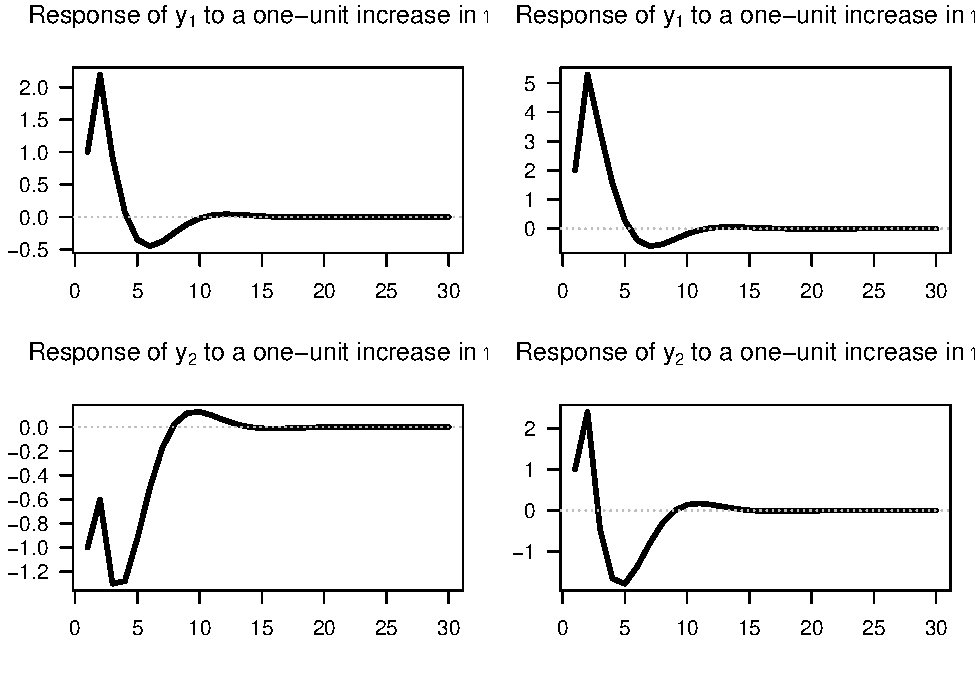
\includegraphics[width=0.95\linewidth]{AdvECTS_files/figure-latex/simVAR-1} \caption{Impulse response functions}\label{fig:simVAR}
\end{figure}

\hypertarget{covariance-stationary-varma-models}{%
\subsection{Covariance-stationary VARMA models}\label{covariance-stationary-varma-models}}

Let's come back to the infinite MA case (Eq. \eqref{eq:InfMA}):
\[
y_t = \mu + \sum_{h=0}^\infty \color{blue}{\Psi_{h}} \eta_{t-h}.
\]
For \(y_t\) to be covariance-stationary (and ergodic for the mean), it has to be the case that
\begin{equation}
\sum_{i=0}^\infty \|\Psi_i\| < \infty,\label{eq:condiInfiniteMA}
\end{equation}
where \(\|A\|\) denotes a norm of the matrix \(A\) (e.g.~\(\|A\|=\sqrt{tr(AA')}\)).

This notably implies that if \(y_t\) is stationary (and ergodic for the mean), then \(\|\Psi_h\|\rightarrow 0\) when \(h\) gets large.

What should be satisfied by \(\Phi_k\)'s and \(\Theta_k\)'s for a VARMA-based process (Eq. @ref\{eq:VARMAstd)) to be stationary? The conditions will be similar to that we had in the univariate case (see Prop. \ref{prp:stability}). Let us introduce the following notations:
\begin{eqnarray}
y_t &=& c + \underbrace{\Phi_1 y_{t-1} + \dots +\Phi_p y_{t-p}}_{\color{blue}{\mbox{AR component}}} +  \label{eq:VARMA2}\\
&&\underbrace{B \eta_t+ \Theta_1 B \eta_{t-1}+ \dots+ \Theta_q B \eta_{t-q}}_{\color{red}{\mbox{MA component}}} \nonumber\\
&\Leftrightarrow& \underbrace{(I - \Phi_1 L - \dots - \Phi_p L^p)}_{= \color{blue}{\Phi(L)}}y_t = c +  \underbrace{ \color{red}{(I - \Theta_1 L - \ldots - \Theta_q L^q)}}_{=\color{red}{\Theta(L)}} B \eta_{t}. \nonumber
\end{eqnarray}

Process \(y_t\) is stationary iff the roots of \(\det(\Phi(z))=0\) are strictly outside the unit circle or, equivalently, iff the eigenvalues of
\begin{equation}
\Phi = \left[\begin{array}{cccc}
\Phi_{1} & \Phi_{2} & \cdots & \Phi_{p}\\
I & 0 & \cdots & 0\\
0 & \ddots & 0 & 0\\
0 & 0 & I & 0\end{array}\right]\label{eq:matrixPHI}
\end{equation}
lie strictly within the unit circle.

Hence, as was the case for univariate processes, the covariance-stationarity of a VARMA model depends only on the specification of its AR part.

Let's derive the first two unconditional moments of a (covariance-stationary) VARMA process.

Based on Eq. \eqref{eq:VARMA2}, we have \(\mathbb{E}(\Phi(L)y_t)=c\), which gives \(\Phi(1)\mathbb{E}(y_t)=c\), or::
\[
\mathbb{E}(y_t) = (I - \Phi_1 - \dots - \Phi_p)^{-1}c.
\]
The autocovariances of \(y_t\) can be deduced from the infinite MA representation (Eq. \eqref{eq:InfMA}). We have:
\[
\gamma_j \equiv \mathbb{C}ov(y_t,y_{t-j}) = \sum_{i=j}^\infty \Psi_i \Psi_{i-j}'.
\]
(Note that this infinite sum exists as soon as Eq. \eqref{eq:condiInfiniteMA} is satisfied.)

Conditional means and autocovariances can also be deduced from Eq. \eqref{eq:InfMA}. For \(0 \le h\) and \(0 \le h_1 \le h_2\):
\begin{eqnarray*}
\mathbb{E}_t(y_{t+h}) &=& \mu + \sum_{k=0}^\infty \Psi_{k+h} \eta_{t-k} \\
\mathbb{C}ov_t(y_{t+1+h_1},y_{t+1+h_2}) &=& \sum_{k=0}^{h_1} \Psi_{k}\Psi_{k+h_2-h_1}'.
\end{eqnarray*}

The previous formula implies in particular that the forecasting error \(y_{t+h} - \mathbb{E}_t(y_{t+h})\) has a variance equal to:
\[
\mathbb{V}ar_t(y_{t+h}) = \sum_{k=1}^{h} \Psi_{k}\Psi_{k}'.
\]
Because the \(\eta_t\) are mutually and serially independent (and therefore uncorrelated), we have:
\[
\mathbb{V}ar(\Psi_k \eta_{t-k}) = \mathbb{V}ar\left(\sum_{i=1}^n \psi_{k,i} \eta_{i,t-k}\right)  = \sum_{i=1}^n \psi_{k,i}\psi_{k,i}',
\]
where \(\psi_{k,i}\) denotes the \(i^{th}\) column of \(\Psi_k\).

This suggests the following decomposition of the variance of the forecast error (called \textbf{variance decomposition}):
\[
\mathbb{V}ar_t(y_{t+h}) = \sum_{i=1}^n \underbrace{\sum_{k=1}^{h}  \psi_{k,i}\psi_{k,i}'}_{\mbox{Contribution of $\eta_{i,t}$}}.
\]

Let us now turn to the estimation of VAR(MA) models.

If there is a MA component, OLS regressions yield biased estimates (even for asymptotically large samples).

Assume \(y_t\) follows a VARMA(1,1) model. We have:
\[
y_{i,t} = \phi_i y_{t-1} + \varepsilon_{i,t},
\]
where \(\phi_i\) is the \(i^{th}\) row of \(\Phi_1\), and where \(\varepsilon_{i,t}\) is a linear combination of \(\eta_t\) and \(\eta_{t-1}\).

Since \(y_{t-1}\) (the regressor) is correlated to \(\eta_{t-1}\), it is also correlated to \(\varepsilon_{i,t}\).

The OLS regression of \(y_{i,t}\) on \(y_{t-1}\) yields a biased estimator of \(\phi_i\).

Estimation methods of VARMA models will be presented in Section \ref{Section:AlternII}.

\hypertarget{estimVAR}{%
\subsection{VAR estimation}\label{estimVAR}}

This section discusses the estimation of VAR models. (The estimation of SVARMA models is more challenging, see, e.g., \citet{Gourieroux_Monfort_Renne_2020}.) Eq. \eqref{eq:yVAR} can be written:
\[
y_{t}=c+\Phi(L)y_{t-1}+\varepsilon_{t},
\]
with \(\Phi(L) = \Phi_1 + \Phi_2 L + \dots + \Phi_p L^{p-1}\).

Consequently:
\[
y_{t}\mid y_{t-1},y_{t-2},\ldots,y_{-p+1}\sim \mathcal{N}(c+\Phi_{1}y_{t-1}+\ldots\Phi_{p}y_{t-p},\Omega).
\]

Using \citet{Hamilton_1994}'s notations, denote with \(\Pi\) the matrix \(\left[\begin{array}{ccccc} c & \Phi_{1} & \Phi_{2} & \ldots & \Phi_{p}\end{array}\right]'\) and with \(x_{t}\) the vector \(\left[\begin{array}{ccccc} 1 & y'_{t-1} & y'_{t-2} & \ldots & y'_{t-p}\end{array}\right]'\), we have:
\begin{equation}
y_{t}= \Pi'x_{t} + \varepsilon_{t}. \label{eq:PIVAR}
\end{equation}
The previous representation is convenient to discuss the estimation of the VAR model, as parameters are gathered in two matrices only: \(\Pi\) and \(\Omega\).

Let us start with the case where the shocks are Gaussian.

\begin{proposition}[MLE of a Gaussian VAR]
\protect\hypertarget{prp:estimVARGaussian}{}\label{prp:estimVARGaussian}If \(y_t\) follows a VAR(p) (see Definition \ref{def:SVAR}), and if \(\varepsilon_t \sim \,i.i.d.\,\mathcal{N}(0,\Omega)\), then the ML estimate of \(\Pi\), denoted by \(\hat{\Pi}\) (see Eq. \eqref{eq:PIVAR}), is given by
\begin{equation}
\hat{\Pi}=\left[\sum_{t=1}^{T}x_{t}x'_{t}\right]^{-1}\left[\sum_{t=1}^{T}y_{t}'x_{t}\right]= (\mathbf{X}'\mathbf{X})^{-1}\mathbf{X}'\mathbf{y},\label{eq:Pi}
\end{equation}
where \(\mathbf{X}\) is the \(T \times (np)\) matrix whose \(t^{th}\) row is \(x_t\) and where \(\mathbf{y}\) is the \(T \times n\) matrix whose \(t^{th}\) row is \(y_{t}'\).

That is, the \(i^{th}\) column of \(\hat{\Pi}\) (\(b_i\), say) is the OLS estimate of \(\beta_i\), where:
\begin{equation}
y_{i,t} = \beta_i'x_t + \varepsilon_{i,t},\label{eq:betayx}
\end{equation}
(i.e., \(\beta_i' = [c_i,\phi_{i,1}',\dots,\phi_{i,p}']'\)).

The ML estimate of \(\Omega\), denoted by \(\hat{\Omega}\), coincides with the sample covariance matrix of the \(n\) series of the OLS residuals in Eq. \eqref{eq:betayx}, i.e.:
\begin{equation}
\hat{\Omega} = \frac{1}{T} \sum_{i=1}^T \hat{\varepsilon}_t\hat{\varepsilon}_t',\quad\mbox{with } \hat{\varepsilon}_t= y_t - \hat{\Pi}'x_t.
\end{equation}

The asymptotic distributions of these estimators are the ones resulting from standard OLS formula.
\end{proposition}

\begin{proof}
See Appendix \ref{estimVARGaussian}.
\end{proof}

As stated by Proposition \ref{OLSVAR}, when the shocks are not Gaussian, then the OLS regressions still provide consistent estimates of the model parameters. However, since \(x_t\) correlates to \(\varepsilon_s\) for \(s<t\), the OLS estimator \(\mathbf{b}_i\) of \(\boldsymbol\beta_i\) is biased in small sample. (That is also the case for the ML estimator.)

Indeed, denoting by \(\boldsymbol\varepsilon_i\) the \(T \times 1\) vector of \(\varepsilon_{i,t}\)'s, and using the notations of \(b_i\) and \(\beta_i\) introduced in Proposition \ref{prp:estimVARGaussian}, we have:
\begin{equation}
\mathbf{b}_i = \beta_i + (\mathbf{X}'\mathbf{X})^{-1}\mathbf{X}'\boldsymbol\varepsilon_i.\label{eq:olsar1}
\end{equation}
We have non-zero correlation between \(x_t\) and \(\varepsilon_{i,s}\) for \(s<t\) and, therefore, \(\mathbb{E}[(\mathbf{X}'\mathbf{X})^{-1}\mathbf{X}'\boldsymbol\varepsilon_i] \ne 0\).

However, when \(y_t\) is covariance stationary, then \(\frac{1}{n}\mathbf{X}'\mathbf{X}\) converges to a positive definite matrix \(\mathbf{Q}\), and \(\frac{1}{n}X'\boldsymbol\varepsilon_i\) converges to 0. Hence \(\mathbf{b}_i \overset{p}{\rightarrow} \beta_i\). More precisely:

\begin{proposition}[Asymptotic distribution of the OLS estimate of $\beta_i$]
\protect\hypertarget{prp:OLSVAR}{}\label{prp:OLSVAR}If \(y_t\) follows a VAR model, as defined in Definition \ref{def:SVAR}, we have:
\[
\sqrt{T}(\mathbf{b}_i-\beta_i) =  \underbrace{\left[\frac{1}{T}\sum_{t=p}^T x_t x_t' \right]^{-1}}_{\overset{p}{\rightarrow} \mathbf{Q}^{-1}}
\underbrace{\sqrt{T} \left[\frac{1}{T}\sum_{t=1}^T x_t\varepsilon_{i,t} \right]}_{\overset{d}{\rightarrow} \mathcal{N}(0,\sigma_i^2\mathbf{Q})},
\]
where \(\sigma_i = \mathbb{V}ar(\varepsilon_{i,t})\) and where \(\mathbf{Q} = \mbox{plim }\frac{1}{T}\sum_{t=p}^T x_t x_t'\) is given by:
\begin{equation}
\mathbf{Q} = \left[
\begin{array}{ccccc}
1 & \mu' &\mu' & \dots & \mu' \\
\mu & \gamma_0 + \mu\mu' & \gamma_1 + \mu\mu' & \dots & \gamma_{p-1} + \mu\mu'\\
\mu & \gamma_1 + \mu\mu' & \gamma_0 + \mu\mu' & \dots & \gamma_{p-2} + \mu\mu'\\
\vdots &\vdots &\vdots &\dots &\vdots \\
\mu & \gamma_{p-1} + \mu\mu' & \gamma_{p-2} + \mu\mu' & \dots & \gamma_{0} + \mu\mu'
\end{array}
\right].\label{eq:Qols}
\end{equation}
\end{proposition}

\begin{proof}
See Appendix \ref{OLSVAR}.
\end{proof}

The following proposition extends the previous proposition and includes covariances between different \(\beta_i\)'s as well as the asymptotic distribution of the ML estimates of \(\Omega\).

\begin{proposition}[Asymptotic distribution of the OLS estimates]
\protect\hypertarget{prp:OLSVAR2}{}\label{prp:OLSVAR2}If \(y_t\) follows a VAR model, as defined in Definition \ref{def:SVAR}, we have:
\begin{equation}
\sqrt{T}\left[
\begin{array}{c}
vec(\hat\Pi - \Pi)\\
vec(\hat\Omega - \Omega)
\end{array}
\right]
\sim \mathcal{N}\left(0,
\left[
\begin{array}{cc}
\Omega \otimes \mathbf{Q}^{-1} & 0\\
0 & \Sigma_{22}
\end{array}
\right]\right),\label{eq:asymptPi}
\end{equation}
where the component of \(\Sigma_{22}\) corresponding to the covariance between \(\hat\sigma_{i,j}\) and \(\hat\sigma_{k,l}\) (for \(i,j,l,m \in \{1,\dots,n\}^4\)) is equal to \(\sigma_{i,l}\sigma_{j,m}+\sigma_{i,m}\sigma_{j,l}\).
\end{proposition}

\begin{proof}
See \citet{Hamilton_1994}, Appendix of Chapter 11.
\end{proof}

Naturally, in practice, \(\Omega\) is replaced by \(\hat{\Omega}\), \(Q\) is replaced with \(\hat{\mathbf{Q}} = \frac{1}{T}\sum_{t=p}^T x_t x_t'\) and \(\Sigma\) with the matrix whose components are of the form \(\hat\sigma_{i,l}\hat\sigma_{j,m}+\hat\sigma_{i,m}\hat\sigma_{j,l}\), where the \(\hat\sigma_{i,l}\)'s are the components of \(\hat\Omega\).

The simplicity of the VAR framework and the tractability of its MLE open the way to convenient econometric testing. Let's illustrate this with the likelihood ratio test. The maximum value achieved by the MLE is
\[
\log\mathcal{L}(Y_{T};\hat{\Pi},\hat{\Omega}) = -\frac{Tn}{2}\log(2\pi)+\frac{T}{2}\log\left|\hat{\Omega}^{-1}\right| -\frac{1}{2}\sum_{t=1}^{T}\left[\hat{\varepsilon}_{t}'\hat{\Omega}^{-1}\hat{\varepsilon}_{t}\right].
\]
The last term is:
\begin{eqnarray*}
\sum_{t=1}^{T}\hat{\varepsilon}_{t}'\hat{\Omega}^{-1}\hat{\varepsilon}_{t} &=& \mbox{Tr}\left[\sum_{t=1}^{T}\hat{\varepsilon}_{t}'\hat{\Omega}^{-1}\hat{\varepsilon}_{t}\right] = \mbox{Tr}\left[\sum_{t=1}^{T}\hat{\Omega}^{-1}\hat{\varepsilon}_{t}\hat{\varepsilon}_{t}'\right]\\
&=&\mbox{Tr}\left[\hat{\Omega}^{-1}\sum_{t=1}^{T}\hat{\varepsilon}_{t}\hat{\varepsilon}_{t}'\right] = \mbox{Tr}\left[\hat{\Omega}^{-1}\left(T\hat{\Omega}\right)\right]=Tn.
\end{eqnarray*}
Therefore, the optimized log-likelihood is simply obtained by:
\begin{equation}
\log\mathcal{L}(Y_{T};\hat{\Pi},\hat{\Omega})=-(Tn/2)\log(2\pi)+(T/2)\log\left|\hat{\Omega}^{-1}\right|-Tn/2.\label{eq:optimzedLogL}
\end{equation}

Assume that we want to test the null hypothesis that a set of variables follows a VAR(\(p_{0}\)) against the alternative
specification of \(p_{1}\) (\(>p_{0}\)).

Let us denote by \(\hat{L}_{0}\) and \(\hat{L}_{1}\) the maximum log-likelihoods obtained with \(p_{0}\) and \(p_{1}\) lags, respectively.

Under the null hypothesis (\(H_0\): \(p=p_0\)), we have:
\begin{eqnarray*}
2\left(\hat{L}_{1}-\hat{L}_{0}\right)&=&T\left(\log\left|\hat{\Omega}_{1}^{-1}\right|-\log\left|\hat{\Omega}_{0}^{-1}\right|\right)  \sim \chi^2(n^{2}(p_{1}-p_{0})).
\end{eqnarray*}

What precedes can be used to help determine the appropriate number of lags to use in the specification. In a VAR, using too many lags consumes numerous degrees of freedom: with \(p\) lags, each of the \(n\) equations in the VAR contains \(n\times p\) coefficients plus the intercept term. Adding lags improve in-sample fit, but is likely to result in over-parameterization and affect the \textbf{out-of-sample} prediction performance.

To select appropriate lag length, \textbf{selection criteria} can be used (see Definition \ref{def:infocriteria}). In the context of VAR models, using Eq. \eqref{eq:optimzedLogL}, we have:
\begin{eqnarray*}
AIC & = & cst + \log\left|\hat{\Omega}\right|+\frac{2}{T}N\\
BIC & = & cst + \log\left|\hat{\Omega}\right|+\frac{\log T}{T}N,
\end{eqnarray*}
where \(N=p \times n^{2}\).

\hypertarget{BlockGranger}{%
\subsection{Block exogeneity and Granger causality}\label{BlockGranger}}

\textbf{Block exogeneity}

Let's decompose \(y_t\) into two subvectors \(y^{(1)}_{t}\) (\(n_1 \times 1\)) and \(y^{(2)}_{t}\) (\(n_2 \times 1\)), with \(y_t' = [{y^{(1)}_{t}}',{y^{(2)}_{t}}']\) (and therefore \(n=n_1 +n_2\)), such that:
\[
\left[
\begin{array}{c}
y^{(1)}_{t}\\
y^{(2)}_{t}
\end{array}
\right] = \left[
\begin{array}{cc}
\Phi^{(1,1)} & \Phi^{(1,2)}\\
\Phi^{(2,1)} & \Phi^{(2,2)}
\end{array}
\right]
\left[
\begin{array}{c}
y^{(1)}_{t-1}\\
y^{(2)}_{t-1}
\end{array}
\right] + \varepsilon_t.
\]
Using, e.g., a likelihood ratio test (see Def. \ref{def:LR}), one can easily test for block exogeneity of \(y_t^{(2)}\) (say). The null assumption can be expressed as \(\Phi^{(2,1)}=0\) and \(\Sigma^{(2,1)}=0\).

\textbf{Granger Causality}

\citet{Granger_1969} developed a method to explore \textbf{causal relationships} among variables. The approach consists in determining whether the past values of \(y_{1,t}\) can help explain the current \(y_{2,t}\) (beyond the information already included in the past values of \(y_{2,t}\)).

Formally, let us denote three information sets:
\begin{eqnarray*}
\mathcal{I}_{1,t} & = & \left\{ y_{1,t},y_{1,t-1},\ldots\right\} \\
\mathcal{I}_{2,t} & = & \left\{ y_{2,t},y_{2,t-1},\ldots\right\} \\
\mathcal{I}_{t} & = & \left\{ y_{1,t},y_{1,t-1},\ldots y_{2,t},y_{2,t-1},\ldots\right\}.
\end{eqnarray*}
We say that \(y_{1,t}\) Granger-causes \(y_{2,t}\) if
\[
\mathbb{E}\left[y_{2,t}\mid \mathcal{I}_{2,t-1}\right]\neq \mathbb{E}\left[y_{2,t}\mid \mathcal{I}_{t-1}\right].
\]

To get the intuition behind the testing procedure, consider the following
bivariate VAR(\(p\)) process:
\begin{eqnarray*}
y_{1,t} & = & c_1+\Sigma_{i=1}^{p}\Phi_i^{(11)}y_{1,t-i}+\Sigma_{i=1}^{p}\Phi_i^{(12)}y_{2,t-i}+\varepsilon_{1,t}\\
y_{2,t} & = & c_2+\Sigma_{i=1}^{p}\Phi_i^{(21)}y_{1,t-i}+\Sigma_{i=1}^{p}\Phi_i^{(22)}y_{2,t-i}+\varepsilon_{2,t},
\end{eqnarray*}
where \(\Phi_k^{(ij)}\) denotes the element \((i,j)\) of \(\Phi_k\).

Then, \(y_{1,t}\) is said not to Granger-cause \(y_{2,t}\) if
\[
\Phi_1^{(21)}=\Phi_2^{(21)}=\ldots=\Phi_p^{(21)}=0.
\]
Therefore the hypothesis testing is
\[
\begin{cases}
H_{0}: & \Phi_1^{(21)}=\Phi_2^{(21)}=\ldots=\Phi_p^{(21)}=0\\
H_{1}: & \Phi_1^{(21)}\neq0\mbox{ or }\Phi_2^{(21)}\neq0\mbox{ or}\ldots\Phi_p^{(21)}\neq0.\end{cases}
\]
Loosely speaking, we reject \(H_{0}\) if some of the coefficients on the lagged \(y_{1,t}\)'s are statistically significant. Formally, this can be tested using the \(F\)-test or asymptotic chi-square test. The \(F\)-statistic is
\[
F=\frac{(RSS-USS)/p}{USS/(T-2p-1)},
\]
where RSS is the Restricted sum of squared residuals and USS is the Unrestricted sum of squared residuals. Under \(H_{0}\), the \(F\)-statistic is distributed as \(\mathcal{F}(p,T-2p-1)\).

Note that \(pF\underset{T \rightarrow \infty}{\rightarrow}\chi^{2}(p)\). Therefore, for large samples and under \(H_0\):
\[
F \sim \chi^{2}(p)/p.
\]

\hypertarget{identification-problem-and-standard-identification-techniques}{%
\subsection{Identification problem and standard identification techniques}\label{identification-problem-and-standard-identification-techniques}}

\textbf{The Identification Issue}

In Section \ref{estimVAR}, we have seen how to estimate \(\mathbb{V}ar(\varepsilon_t) =\Omega\) and the \(\Phi_k\) matrices in the context of a VAR model. But the IRFs are functions of \(B\) and the \(\Phi_k\)'s, not of \(\Omega\) the \(\Phi_k\)'s (see Section \ref{IRFSVARMA}). We have \(\Omega = BB'\), but this is not sufficient to recover \(B\).

Indeed, seen a system of equations whose unknowns are the \(b_{i,j}\)'s (components of \(B\)), the system \(\Omega = BB'\) contains only \(n(n+1)/2\) linearly independent equations. For instance, for \(n=2\):
\begin{eqnarray*}
&&\left[
\begin{array}{cc}
\omega_{11} & \omega_{12} \\
\omega_{12} & \omega_{22}
\end{array}
\right] = \left[
\begin{array}{cc}
b_{11} & b_{12} \\
b_{21} & b_{22}
\end{array}
\right]\left[
\begin{array}{cc}
b_{11} & b_{21} \\
b_{12} & b_{22}
\end{array}
\right]\\
&\Leftrightarrow&\left[
\begin{array}{cc}
\omega_{11} & \omega_{12} \\
\omega_{12} & \omega_{22}
\end{array}
\right] = \left[
\begin{array}{cc}
b_{11}^2+b_{12}^2 & \color{red}{b_{11}b_{21}+b_{12}b_{22}} \\
\color{red}{b_{11}b_{21}+b_{12}b_{22}} & b_{22}^2 + b_{21}^2
\end{array}
\right].
\end{eqnarray*}

We then have 3 linearly independent equations but 4 unknowns. Therefore, \(B\) is not identified based on second-order moments. Additional restrictions are required to identify \(B\).

This section covers two standard identification schemes: \textbf{short-run} and \textbf{long-run} restrictions:

\begin{enumerate}
\def\labelenumi{\arabic{enumi}.}
\tightlist
\item
  a \textbf{short-run restriction (SRR)} prevents a structural shock from affecting an endogenous variable contemporaneously.
\end{enumerate}

\begin{itemize}
\tightlist
\item
  Easy to implement: the appropriate entries of \(B\) are set to 0.
\item
  Particular case: \textbf{Cholesky, or recursive approach}.
\item
  Examples: \citet{BERNANKE198649}, \citet{Sims_1986}, \citet{Gali_1992}, \citet{RubioRamirez_et_al_2010}.
\end{itemize}

\begin{enumerate}
\def\labelenumi{\arabic{enumi}.}
\setcounter{enumi}{1}
\tightlist
\item
  a \textbf{long-run restriction (LRR)} prevents a structural shock from having a cumulative impact on one of the endogenous variables.
\end{enumerate}

\begin{itemize}
\tightlist
\item
  Additional computations are required to implement this. One needs to compute the cumulative effect of one of the structural shocks \(u_{t}\) on one of the endogenous variable.
\item
  Examples: \citet{Blanchard_Quah_1989}, \citet{Faust_Leeper_1997}, \citet{Gali_1999}, \citet{Erceg_et_al_2005}, \citet{NBERc11177}.
\end{itemize}

The two approaches can be combined (see, e.g., \citet{Gerlach_Smets_1995}).

Let us consider a simple exmaple that could motivate short-run restrictions. Consider the following stylized macro model:
\begin{equation}
\begin{array}{clll}
g_{t}&=& \bar{g}-\lambda(i_{t-1}-\mathbb{E}_{t-1}\pi_{t})+ \underbrace{{\color{blue}\sigma_d \eta_{d,t}}}_{\mbox{demand shock}}& (\mbox{IS curve})\\
\Delta \pi_{t} & = & \beta (g_{t} - \bar{g})+ \underbrace{{\color{blue}\sigma_{\pi} \eta_{\pi,t}}}_{\mbox{cost push shock}} & (\mbox{Phillips curve})\\
i_{t} & = & \rho i_{t-1} + \left[ \gamma_\pi \mathbb{E}_{t}\pi_{t+1}  + \gamma_g (g_{t} - \bar{g}) \right]\\
&& \qquad \qquad+\underbrace{{\color{blue}\sigma_{mp} \eta_{mp,t}}}_{\mbox{Mon. Pol. shock}} & (\mbox{Taylor rule}),
\end{array}\label{eq:systemI}
\end{equation}
where:
\begin{equation}
\eta_t = 
\left[
\begin{array}{c}
\eta_{\pi,t}\\
\eta_{d,t}\\
\eta_{mp,t}
\end{array}
\right]
\sim i.i.d.\,\mathcal{N}(0,I).\label{eq:covU}
\end{equation}

Vector \(\eta_t\) is assumed to be a vector of structural shocks, mutually and serially independent. On date \(t\):

\begin{itemize}
\tightlist
\item
  \(g_t\) is contemporaneously affected by \(\eta_{d,t}\) only;
\item
  \(\pi_t\) is contemporaneously affected by \(\eta_{\pi,t}\) and \(\eta_{d,t}\);
\item
  \(i_t\) is contemporaneously affected by \(\eta_{mp,t}\), \(\eta_{\pi,t}\) and \(\eta_{d,t}\).
\end{itemize}

System \eqref{eq:systemI} could be rewritten in the form:
\begin{equation}
\left[\begin{array}{c}
d_t\\
\pi_t\\
i_t
\end{array}\right]
= \Phi(L)
\left[\begin{array}{c}
d_{t-1}\\
\pi_{t-1}\\
i_{t-1} +
\end{array}\right] +\underbrace{\underbrace{
\left[
\begin{array}{ccc}
0 & \bullet & 0 \\
\bullet & \bullet & 0 \\
\bullet & \bullet & \bullet
\end{array}
\right]}_{=B} \eta_t}_{=\varepsilon_t}\label{eq:BBBB}
\end{equation}

This is the \textbf{reduced-form} of the model. This representation suggests three additional restrictions on the entries of \(B\); the latter matrix is therefore identified (up to the signs of its columns) as soon as \(\Omega = BB'\) is known.

There are particular cases in which some well-known matrix decomposition of \(\Omega=\mathbb{V}ar(\varepsilon_t)\) can be used to easily estimate some specific SVAR.

Consider the following context:

\begin{itemize}
\tightlist
\item
  A first shock (say, \(\eta_{n_1,t}\)) can affect instantaneously
  (i.e., on date \(t\)) only one of the endogenous variable (say, \(y_{n_1,t}\));
\item
  A second shock (say, \(\eta_{n_2,t}\)) can affect instantaneously
  (i.e., on date \(t\)) the first two endogenous variables (say, \(y_{n_1,t}\)
  and \(y_{n_2,t}\));
\item
  \ldots{}
\end{itemize}

This implies (1) that column \(n_1\) of \(B\) has only 1 non-zero entry (this is the \(n_1^{th}\) entry), (2) that column \(n_2\) of \(B\) has 2 non-zero entries (the \(n_1^{th}\) and the \(n_2^{th}\) ones), etc. Without loss of generality, we can set \(n_1=n\), \(n_2=n-1\), etc. In this context, matrix \(B\) is lower triangular.

The Cholesky decomposition of \(\Omega_{\varepsilon}\) then provides an appropriate estimate of \(B\), that is a lower triangular matrix \(B\) that is such that:
\[
\Omega_\varepsilon = BB'.
\]

For instance, \citet{DEDOLA20051543} estimate 5 structural VAR models for the US, the UK, Germany, France and Italy to analyse the monetary-policy transmission mechanisms. They estimate SVAR(5) models over the period 1975-1997. The shock-identification scheme is based on Cholesky decompositions, the ordering of the endogenous variables being: the industrial production, the consumer price index, a commodity price index, the short-term rate, monetary aggregate and the effective exchange rate (except for the US). This ordering implies that monetary policy reacts to the shocks affecting the first three variables but that the latter react to monetary policy shocks with a one-period lag only.

Importantly, the Cholesky approach can be useful when one is interested in one specific structural shock. This was the case, e.g., of \citet{Christiano_Eichenbaum_Evans_1996}. Their identification is based on the following relationship between \(\varepsilon_t\) and \(\eta_t\):
\[
\left[\begin{array}{c}
\boldsymbol\varepsilon_{S,t}\\
\varepsilon_{r,t}\\
\boldsymbol\varepsilon_{F,t}
\end{array}\right] =
\left[\begin{array}{ccc}
B_{SS} & 0 & 0 \\
B_{rS} & B_{rr} & 0 \\
B_{FS} & B_{Fr} & B_{FF}
\end{array}\right]
\left[\begin{array}{c}
\boldsymbol\eta_{S,t}\\
\eta_{r,t}\\
\boldsymbol\eta_{F,t}
\end{array}\right],
\]
where \(S\), \(r\) and \(F\) respectively correspond to \emph{slow-moving variables}, the policy variable (short-term rate) and \emph{fast-moving variables}. While \(\eta_{r,t}\) is scalar, \(\boldsymbol\eta_{S,t}\) and \(\boldsymbol\eta_{F,t}\) may be vectors. The space spanned by \(\boldsymbol\varepsilon_{S,t}\) is the same as that spanned by \(\boldsymbol\eta_{S,t}\). As a result, because \(\varepsilon_{r,t}\) is a linear combination of \(\eta_{r,t}\) and \(\boldsymbol\eta_{S,t}\) (which are \(\perp\)), it comes that the \(B_{rr}\eta_{r,t}\)'s are the (population) residuals in the regression of \(\varepsilon_{r,t}\) on \(\boldsymbol\varepsilon_{S,t}\). Because \(\mathbb{V}ar(\eta_{r,t})=1\), \(B_{rr}\) is given by the square root of the variance of \(B_{rr}\eta_{r,t}\). \(B_{F,r}\) is finally obtained by regressing the components of \(\boldsymbol\varepsilon_{F,t}\) on \(\eta_{r,t}\).

An equivalent approach consists in computing the Cholesky decomposition of \(BB'\) and the contemporaneous impacts of the monetary policy shock (on the \(n\) endogenous variables) are the components of the column of \(B\) corresponding to the policy variable.

\begin{Shaded}
\begin{Highlighting}[]
\FunctionTok{library}\NormalTok{(AEC)}
\FunctionTok{data}\NormalTok{(}\StringTok{"USmonthly"}\NormalTok{)}
\CommentTok{\# Select sample period:}
\NormalTok{First.date }\OtherTok{\textless{}{-}} \StringTok{"1965{-}01{-}01"}
\NormalTok{Last.date }\OtherTok{\textless{}{-}} \StringTok{"1995{-}06{-}01"}
\NormalTok{indic.first }\OtherTok{\textless{}{-}} \FunctionTok{which}\NormalTok{(USmonthly}\SpecialCharTok{$}\NormalTok{DATES}\SpecialCharTok{==}\NormalTok{First.date)}
\NormalTok{indic.last  }\OtherTok{\textless{}{-}} \FunctionTok{which}\NormalTok{(USmonthly}\SpecialCharTok{$}\NormalTok{DATES}\SpecialCharTok{==}\NormalTok{Last.date)}
\NormalTok{USmonthly   }\OtherTok{\textless{}{-}}\NormalTok{ USmonthly[indic.first}\SpecialCharTok{:}\NormalTok{indic.last,]}
\NormalTok{considered.variables }\OtherTok{\textless{}{-}} \FunctionTok{c}\NormalTok{(}\StringTok{"LIP"}\NormalTok{,}\StringTok{"UNEMP"}\NormalTok{,}\StringTok{"LCPI"}\NormalTok{,}\StringTok{"LPCOM"}\NormalTok{,}\StringTok{"FFR"}\NormalTok{,}\StringTok{"NBR"}\NormalTok{,}\StringTok{"TTR"}\NormalTok{,}\StringTok{"M1"}\NormalTok{)}
\NormalTok{y }\OtherTok{\textless{}{-}} \FunctionTok{as.matrix}\NormalTok{(USmonthly[considered.variables])}
\NormalTok{res.svar.ordering }\OtherTok{\textless{}{-}} \FunctionTok{svar.ordering}\NormalTok{(y,}\AttributeTok{p=}\DecValTok{3}\NormalTok{,}
                                   \AttributeTok{posit.of.shock =} \DecValTok{5}\NormalTok{,}
                                   \AttributeTok{nb.periods.IRF =} \DecValTok{20}\NormalTok{,}
                                   \AttributeTok{nb.bootstrap.replications =} \DecValTok{100}\NormalTok{, }\CommentTok{\# This is used in the parametric bootstrap only}
                                   \AttributeTok{confidence.interval =} \FloatTok{0.90}\NormalTok{, }\CommentTok{\# expressed in pp.}
                                   \AttributeTok{indic.plot =} \DecValTok{1} \CommentTok{\# Plots are displayed if = 1.}
\NormalTok{)}
\end{Highlighting}
\end{Shaded}

\begin{figure}
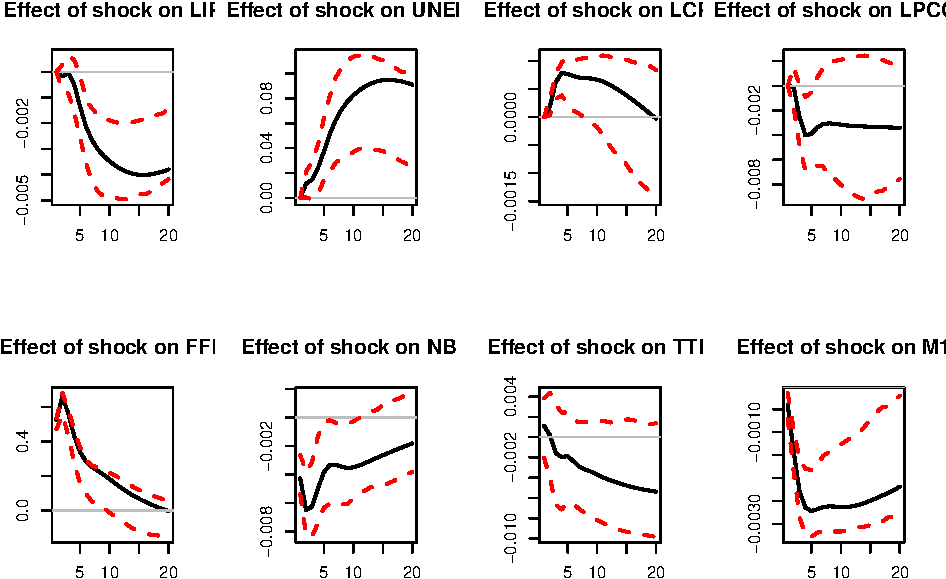
\includegraphics[width=0.95\linewidth]{AdvECTS_files/figure-latex/CEE-1} \caption{Response to a monetary-policy shock. Identification approach of Christiano, Eichenbaum and Evans (1996).}\label{fig:CEE}
\end{figure}

Let us now turn to \textbf{Long-run restrictions}. Such a restriction concerns the long-run influence of a shock on an endogenous variable. Let us consider for instance a structural shock that is assumed to have no ``long-run influence'' on GDP. How to express this? The long-run change in GDP can be expressed as \(GDP_{t+h} - GDP_t\), with \(h\) large. Note further that:
\[
GDP_{t+h} - GDP_t = \Delta GDP_{t+h} +\Delta GDP_{t+h-1} + \dots + \Delta GDP_{t+1}.
\]
Hence, the fact that a given structural shock (\(\eta_{i,t}\), say) has no long-run influence on GDP means that
\[
\lim_{h\rightarrow\infty}\frac{\partial GDP_{t+h}}{\partial \eta_{i,t}} = \lim_{h\rightarrow\infty} \frac{\partial}{\partial \eta_{i,t}}\left(\sum_{k=1}^h \Delta  GDP_{t+k}\right)= 0.
\]

This can be easily formulated as a function of \(B\) and of the matrices \(\Phi_i\) when \(y_t\) (including \(\Delta GDP_t\)) follows a VAR process.

Without loss of generality, we will only consider the VAR(1) case. Indeed, one can always write a VAR(\(p\)) as a VAR(1). To see that, stack the last \(p\) values of vector \(y_t\) in vector \(y_{t}^{*}=[y_t',\dots,y_{t-p+1}']'\); Eq. \eqref{eq:yVAR} can then be rewritten in its companion form:
\begin{equation}
y_{t}^{*} =
\underbrace{\left[\begin{array}{c}
c\\
0\\
\vdots\\
0\end{array}\right]}_{=c^*}+
\underbrace{\left[\begin{array}{cccc}
\Phi_{1} & \Phi_{2} & \cdots & \Phi_{p}\\
I & 0 & \cdots & 0\\
0 & \ddots & 0 & 0\\
0 & 0 & I & 0\end{array}\right]}_{=\Phi}
y_{t-1}^{*}+
\underbrace{\left[\begin{array}{c}
\varepsilon_{t}\\
0\\
\vdots\\
0\end{array}\right]}_{\varepsilon_t^*},\label{eq:ystarVAR}
\end{equation}
where matrices \(\Phi\) and \(\Omega^* = \mathbb{V}ar(\varepsilon_t^*)\) are of dimension \(np \times np\); \(\Omega^*\) is filled with zeros, except the \(n\times n\) upper-left block that is equal to \(\Omega = \mathbb{V}ar(\varepsilon_t)\). (Matrix \(\Phi\) had been introduced in Eq. \eqref{eq:matrixPHI}.)

Focusing on the VAR(1) case:
\begin{eqnarray}
y_{t} &=& c+\Phi y_{t-1}+\varepsilon_{t}\\
& = & c+\varepsilon_{t}+\Phi(c+\varepsilon_{t-1})+\ldots+\Phi^{k}(c+\varepsilon_{t-k})+\ldots \nonumber \\
& = & \mu +\varepsilon_{t}+\Phi\varepsilon_{t-1}+\ldots+\Phi^{k}\varepsilon_{t-k}+\ldots \\
& = & \mu +B\eta_{t}+\Phi B\eta_{t-1}+\ldots+\Phi^{k}B\eta_{t-k}+\ldots,
\end{eqnarray}

The sequence of shocks \(\{\eta_t\}\) determines the sequence \(\{y_t\}\). What if \(\{\eta_t\}\) is replaced by \(\{\tilde{\eta}_t\}\), where \(\tilde{\eta}_t=\eta_t\) if \(t \ne s\) and \(\tilde{\eta}_s=\eta_s + \gamma\)?

Assume \(\{\tilde{y}_t\}\) is the associated ``perturbated'' sequence. We have \(\tilde{y}_t = y_t\) if \(t<s\). For \(t \ge s\), the Wold decomposition of \(\{\tilde{y}_t\}\) implies:
\[
\tilde{y}_t = y_t + \Phi^{t-s} B \gamma.
\]
Therefore, the cumulative impact of \(\gamma\) on \(\tilde{y}_t\) will be (for \(t \ge s\)):
\begin{eqnarray}
(\tilde{y}_t - y_t) +  (\tilde{y}_{t-1} - y_{t-1}) + \dots +  (\tilde{y}_s - y_s) &=& \nonumber \\
(Id + \Phi + \Phi^2 + \dots + \Phi^{t-s}) B \gamma.&& \label{eq:cumul}
\end{eqnarray}

Consider a shock on \(\eta_{1,t}\), with a magnitude of \(1\). This shock corresponds to \(\gamma = [1,0,\dots,0]'\). Given Eq. \eqref{eq:cumul}, the long-run cumulative effect of this shock on the endogenous variables is given by:
\[
\underbrace{(Id+\Phi+\ldots+\Phi^{k}+\ldots)}_{=(Id - \Phi)^{-1}}B\left[\begin{array}{c}
1\\
0\\
\vdots\\
0\end{array}\right],
\]
that is the first column of \(\Theta \equiv (Id - \Phi)^{-1}B\).

In this context, consider the following long-run restriction: \emph{``\(j^{th}\) structural shock has no cumulative impact on the \(i^{th}\) endogenous variable''}. It is equivalent to
\[
\Theta_{ij}=0,
\]
where \(\Theta_{ij}\) is the element \((i,j)\) of \(\Theta\).

\citet{Blanchard_Quah_1989} implement long-run restrictions in a small-scale VAR. Two variables are considered: GDP and unemployment. Consequently, the VAR is affected by two types of shocks. The authors want to identify \textbf{supply shocks} (that can have a permanent effect on output) and \textbf{demand shocks} (that cannot have a permanent effect on output).\footnote{The motivation of the authors regarding their long-run restrictions can be obtained from a traditional Keynesian view of fluctuations. The authors propose a variant of a model from \citet{Fischer_1977}.
}

\citet{Blanchard_Quah_1989}'s dataset is quarterly, spanning the period from 1950:2 to 1987:4. Their VAR features 8 lags. Here are the data they use:

\begin{Shaded}
\begin{Highlighting}[]
\FunctionTok{library}\NormalTok{(AEC)}
\FunctionTok{par}\NormalTok{(}\AttributeTok{mfrow=}\FunctionTok{c}\NormalTok{(}\DecValTok{1}\NormalTok{,}\DecValTok{2}\NormalTok{))}
\FunctionTok{plot}\NormalTok{(BQ}\SpecialCharTok{$}\NormalTok{Date,BQ}\SpecialCharTok{$}\NormalTok{Dgdp,}\AttributeTok{type=}\StringTok{"l"}\NormalTok{,}\AttributeTok{main=}\StringTok{"GDP quarterly growth rate"}\NormalTok{,}\AttributeTok{xlab=}\StringTok{""}\NormalTok{,}\AttributeTok{ylab=}\StringTok{""}\NormalTok{,}\AttributeTok{lwd=}\DecValTok{2}\NormalTok{)}
\FunctionTok{plot}\NormalTok{(BQ}\SpecialCharTok{$}\NormalTok{Date,BQ}\SpecialCharTok{$}\NormalTok{unemp,}\AttributeTok{type=}\StringTok{"l"}\NormalTok{,}\AttributeTok{ylim=}\FunctionTok{c}\NormalTok{(}\SpecialCharTok{{-}}\DecValTok{3}\NormalTok{,}\DecValTok{6}\NormalTok{),}\AttributeTok{main=}\StringTok{"Unemployment rate (gap)"}\NormalTok{,}\AttributeTok{xlab=}\StringTok{""}\NormalTok{,}\AttributeTok{ylab=}\StringTok{""}\NormalTok{,}\AttributeTok{lwd=}\DecValTok{2}\NormalTok{)}
\end{Highlighting}
\end{Shaded}

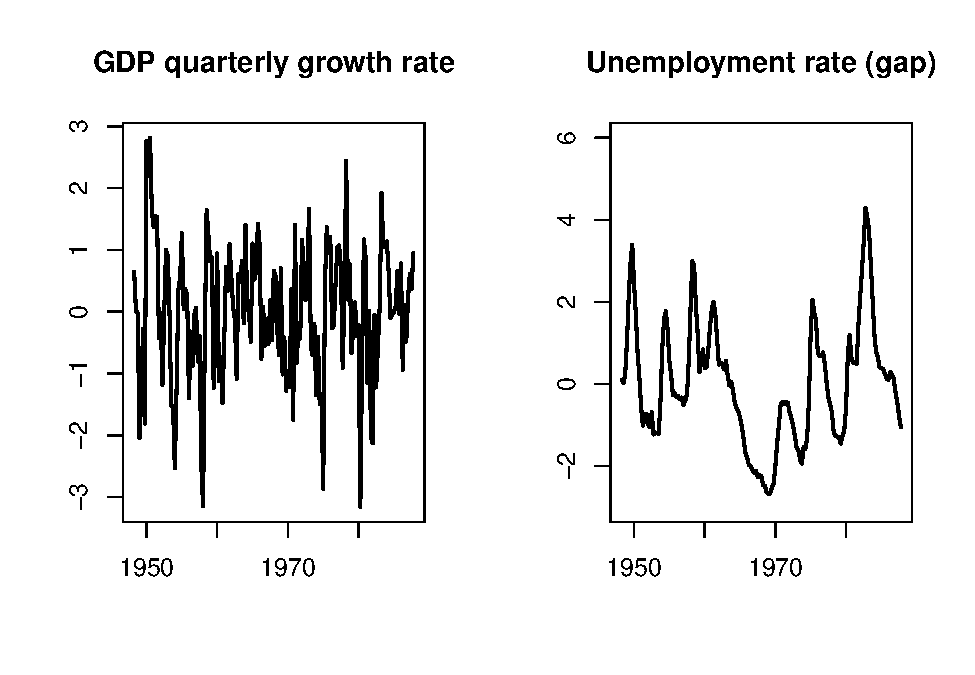
\includegraphics{AdvECTS_files/figure-latex/BQ1-1.pdf}

Estimate a reduced-form VAR(8) model:

\begin{Shaded}
\begin{Highlighting}[]
\FunctionTok{library}\NormalTok{(vars)}
\NormalTok{y }\OtherTok{\textless{}{-}}\NormalTok{ BQ[,}\DecValTok{2}\SpecialCharTok{:}\DecValTok{3}\NormalTok{]}
\NormalTok{est.VAR }\OtherTok{\textless{}{-}} \FunctionTok{VAR}\NormalTok{(y,}\AttributeTok{p=}\DecValTok{8}\NormalTok{)}
\NormalTok{Omega }\OtherTok{\textless{}{-}} \FunctionTok{var}\NormalTok{(}\FunctionTok{residuals}\NormalTok{(est.VAR))}
\end{Highlighting}
\end{Shaded}

Now, let us define a loss function (\texttt{loss}) that is equal to zero if (a) \(BB'=\Omega\) and (b) the element (1,1) of \(\Theta B\) is equal to zero:

\begin{Shaded}
\begin{Highlighting}[]
\CommentTok{\# Compute (Id {-} Phi)\^{}\{{-}1\}:}
\NormalTok{Phi }\OtherTok{\textless{}{-}} \FunctionTok{Acoef}\NormalTok{(est.VAR)}
\NormalTok{PHI }\OtherTok{\textless{}{-}} \FunctionTok{make.PHI}\NormalTok{(Phi)}
\NormalTok{sum.PHI.k }\OtherTok{\textless{}{-}} \FunctionTok{solve}\NormalTok{(}\FunctionTok{diag}\NormalTok{(}\FunctionTok{dim}\NormalTok{(PHI)[}\DecValTok{1}\NormalTok{]) }\SpecialCharTok{{-}}\NormalTok{ PHI)[}\DecValTok{1}\SpecialCharTok{:}\DecValTok{2}\NormalTok{,}\DecValTok{1}\SpecialCharTok{:}\DecValTok{2}\NormalTok{]}
\NormalTok{loss }\OtherTok{\textless{}{-}} \ControlFlowTok{function}\NormalTok{(param)\{}
\NormalTok{  B }\OtherTok{\textless{}{-}} \FunctionTok{matrix}\NormalTok{(param,}\DecValTok{2}\NormalTok{,}\DecValTok{2}\NormalTok{)}
\NormalTok{  X }\OtherTok{\textless{}{-}}\NormalTok{ Omega }\SpecialCharTok{{-}}\NormalTok{ B }\SpecialCharTok{\%*\%} \FunctionTok{t}\NormalTok{(B)}
\NormalTok{  Theta }\OtherTok{\textless{}{-}}\NormalTok{ sum.PHI.k[}\DecValTok{1}\SpecialCharTok{:}\DecValTok{2}\NormalTok{,}\DecValTok{1}\SpecialCharTok{:}\DecValTok{2}\NormalTok{] }\SpecialCharTok{\%*\%}\NormalTok{ B}
\NormalTok{  loss }\OtherTok{\textless{}{-}} \DecValTok{10000} \SpecialCharTok{*}\NormalTok{ ( X[}\DecValTok{1}\NormalTok{,}\DecValTok{1}\NormalTok{]}\SpecialCharTok{\^{}}\DecValTok{2} \SpecialCharTok{+}\NormalTok{ X[}\DecValTok{2}\NormalTok{,}\DecValTok{1}\NormalTok{]}\SpecialCharTok{\^{}}\DecValTok{2} \SpecialCharTok{+}\NormalTok{ X[}\DecValTok{2}\NormalTok{,}\DecValTok{2}\NormalTok{]}\SpecialCharTok{\^{}}\DecValTok{2} \SpecialCharTok{+}\NormalTok{ Theta[}\DecValTok{1}\NormalTok{,}\DecValTok{1}\NormalTok{]}\SpecialCharTok{\^{}}\DecValTok{2}\NormalTok{ )}
  \FunctionTok{return}\NormalTok{(loss)}
\NormalTok{\}}
\NormalTok{res.opt }\OtherTok{\textless{}{-}} \FunctionTok{optim}\NormalTok{(}\FunctionTok{c}\NormalTok{(}\DecValTok{1}\NormalTok{,}\DecValTok{0}\NormalTok{,}\DecValTok{0}\NormalTok{,}\DecValTok{1}\NormalTok{),loss,}\AttributeTok{method=}\StringTok{"BFGS"}\NormalTok{,}\AttributeTok{hessian=}\ConstantTok{FALSE}\NormalTok{)}
\FunctionTok{print}\NormalTok{(res.opt}\SpecialCharTok{$}\NormalTok{par)}
\end{Highlighting}
\end{Shaded}

\begin{verbatim}
## [1]  0.8570358 -0.2396345  0.1541395  0.1921221
\end{verbatim}

(Note: one can use that type of approach, based on a loss function, to mix short- and long-run restrictions.)

Figure \ref{fig:BQ4} displays the resulting IRFs. Note that, for GDP, we cumulate the GDP growth IRF, so as to have the response of the GDP level.

\begin{Shaded}
\begin{Highlighting}[]
\NormalTok{B.hat }\OtherTok{\textless{}{-}} \FunctionTok{matrix}\NormalTok{(res.opt}\SpecialCharTok{$}\NormalTok{par,}\DecValTok{2}\NormalTok{,}\DecValTok{2}\NormalTok{)}
\FunctionTok{print}\NormalTok{(}\FunctionTok{cbind}\NormalTok{(Omega,B.hat }\SpecialCharTok{\%*\%} \FunctionTok{t}\NormalTok{(B.hat)))}
\end{Highlighting}
\end{Shaded}

\begin{verbatim}
##             Dgdp       unemp                       
## Dgdp   0.7582704 -0.17576173  0.7582694 -0.17576173
## unemp -0.1757617  0.09433658 -0.1757617  0.09433558
\end{verbatim}

\begin{Shaded}
\begin{Highlighting}[]
\NormalTok{nb.sim }\OtherTok{\textless{}{-}} \DecValTok{40}
\FunctionTok{par}\NormalTok{(}\AttributeTok{mfrow=}\FunctionTok{c}\NormalTok{(}\DecValTok{2}\NormalTok{,}\DecValTok{2}\NormalTok{))}
\NormalTok{Y }\OtherTok{\textless{}{-}} \FunctionTok{simul.VAR}\NormalTok{(}\AttributeTok{c=}\FunctionTok{matrix}\NormalTok{(}\DecValTok{0}\NormalTok{,}\DecValTok{2}\NormalTok{,}\DecValTok{1}\NormalTok{),Phi,B.hat,nb.sim,}\AttributeTok{y0.star=}\FunctionTok{rep}\NormalTok{(}\DecValTok{0}\NormalTok{,}\DecValTok{2}\SpecialCharTok{*}\DecValTok{8}\NormalTok{),}\AttributeTok{indic.IRF =} \DecValTok{1}\NormalTok{,}\AttributeTok{u.shock =} \FunctionTok{c}\NormalTok{(}\DecValTok{1}\NormalTok{,}\DecValTok{0}\NormalTok{))}
\FunctionTok{plot}\NormalTok{(}\FunctionTok{cumsum}\NormalTok{(Y[,}\DecValTok{1}\NormalTok{]),}\AttributeTok{type=}\StringTok{"l"}\NormalTok{,}\AttributeTok{lwd=}\DecValTok{2}\NormalTok{,}\AttributeTok{xlab=}\StringTok{""}\NormalTok{,}\AttributeTok{ylab=}\StringTok{""}\NormalTok{,}\AttributeTok{main=}\StringTok{"Demand shock on GDP"}\NormalTok{)}
\FunctionTok{plot}\NormalTok{(Y[,}\DecValTok{2}\NormalTok{],}\AttributeTok{type=}\StringTok{"l"}\NormalTok{,}\AttributeTok{lwd=}\DecValTok{2}\NormalTok{,}\AttributeTok{xlab=}\StringTok{""}\NormalTok{,}\AttributeTok{ylab=}\StringTok{""}\NormalTok{,}\AttributeTok{main=}\StringTok{"Demand shock on UNEMP"}\NormalTok{)}
\NormalTok{Y }\OtherTok{\textless{}{-}} \FunctionTok{simul.VAR}\NormalTok{(}\AttributeTok{c=}\FunctionTok{matrix}\NormalTok{(}\DecValTok{0}\NormalTok{,}\DecValTok{2}\NormalTok{,}\DecValTok{1}\NormalTok{),Phi,B.hat,nb.sim,}\AttributeTok{y0.star=}\FunctionTok{rep}\NormalTok{(}\DecValTok{0}\NormalTok{,}\DecValTok{2}\SpecialCharTok{*}\DecValTok{8}\NormalTok{),}\AttributeTok{indic.IRF =} \DecValTok{1}\NormalTok{,}\AttributeTok{u.shock =} \FunctionTok{c}\NormalTok{(}\DecValTok{0}\NormalTok{,}\DecValTok{1}\NormalTok{))}
\FunctionTok{plot}\NormalTok{(}\FunctionTok{cumsum}\NormalTok{(Y[,}\DecValTok{1}\NormalTok{]),}\AttributeTok{type=}\StringTok{"l"}\NormalTok{,}\AttributeTok{lwd=}\DecValTok{2}\NormalTok{,}\AttributeTok{xlab=}\StringTok{""}\NormalTok{,}\AttributeTok{ylab=}\StringTok{""}\NormalTok{,}\AttributeTok{main=}\StringTok{"Supply shock on GDP"}\NormalTok{)}
\FunctionTok{plot}\NormalTok{(Y[,}\DecValTok{2}\NormalTok{],}\AttributeTok{type=}\StringTok{"l"}\NormalTok{,}\AttributeTok{lwd=}\DecValTok{2}\NormalTok{,}\AttributeTok{xlab=}\StringTok{""}\NormalTok{,}\AttributeTok{ylab=}\StringTok{""}\NormalTok{,}\AttributeTok{main=}\StringTok{"Supply shock on UNEMP"}\NormalTok{)}
\end{Highlighting}
\end{Shaded}

\begin{figure}
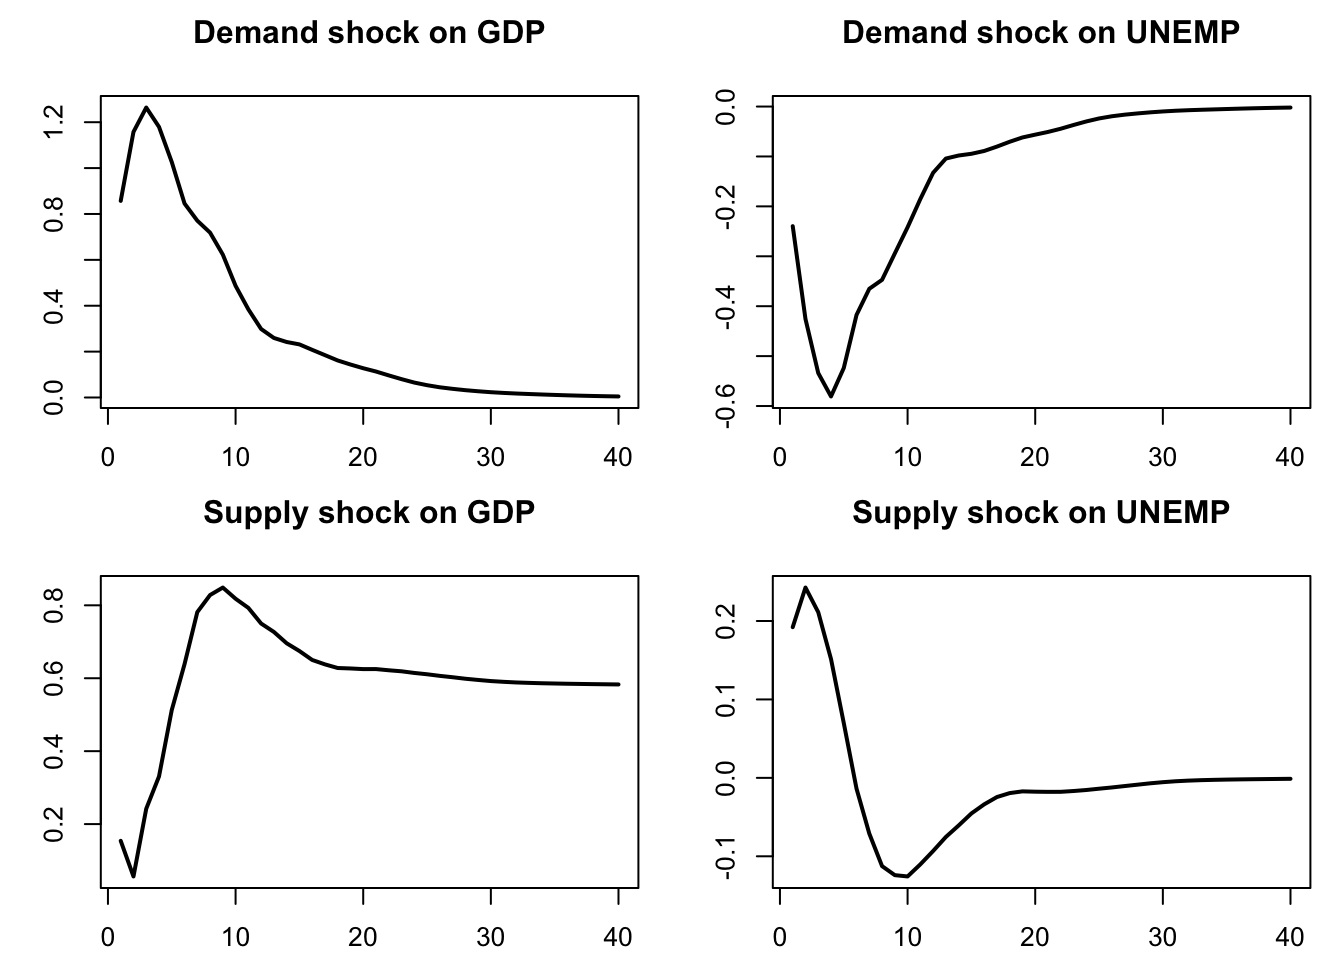
\includegraphics[width=0.95\linewidth]{AdvECTS_files/figure-latex/BQ4-1} \caption{IRF of GDP and unemployment to demand and supply shocks.}\label{fig:BQ4}
\end{figure}

\hypertarget{Signs}{%
\subsection{Sign restrictions}\label{Signs}}

To identifiy the structural shocks, we need to find a matrix \(B\) that satisfies \(\Omega_{\varepsilon} = BB'\) (with \(\Omega = \mathbb{V}ar(\varepsilon_t)\)) and other restrictions. Indeed, \(\Omega_{\varepsilon} = BB'\) is not sufficent to identify \(B\) since, if we take any orthogonal matrix \(Q\) (see Def. \ref{def:orthogonal}), then \(\mathcal{P}=BQ\) also satisfies \(\Omega = \mathcal{P}\mathcal{P}'\).

\begin{definition}[Orthogonal matrix]
\protect\hypertarget{def:orthogonal}{}\label{def:orthogonal}An orthogonal matri \(Q\) is a matrix such that \(QQ' = I,\) i.e., all columns (rows) of \(Q\) are are
orthogonal and unit vectors:
\[q_i'q_j=0\text{ if }i\neq j\text{ and }q_i'q_j=1\text{ if }i= j,\]
where \(q_i\) is the \(i^{th}\) column of \(Q\).
\end{definition}

The idea behind the sign-restriction approach is to ``draw'' random matrices \(\mathcal{P}\) that satisfy \(\Omega = \mathcal{P}\mathcal{P}'\), and then to constitute a set of admissible matrices, keeping in this set only the simulated \(\mathcal{P}\) matrices that satisfy some predefined sign-based restriction. An example of restriction is ``\emph{after one year, a contractionary monetary-policy shocks has a negative impact on inflation}''.

As suggested above, if \(B\) is any matrix that satisfies \(\Omega = BB'\) (for instance, \(B\) can be based on the Cholesky decomposition of \(\Omega\)), then we also have \(\Omega = \mathcal{P}\mathcal{P}'\) as soon as \(\mathcal{P}=BQ\), where \(Q\) is an orthogonal matrix. Therefore, to draw \(\mathcal{P}\) matrices, it suffices to draw in the set of orthogonal matrices.

To fix ideas, consider dimension 2. In that case, the orthogonal matrices are rotation matrices, and the set of orthogonal matrices can be parameterized by the angle \(x\), with:
\[
Q_x=\begin{pmatrix}\cos(x)&\cos\left(x+\frac{\pi}{2}\right)\\
\sin(x)&\sin\left(x+\frac{\pi}{2}\right)\end{pmatrix}=\begin{pmatrix}\cos(x)&-\sin(x)\\
\sin(x)&\cos(x)\end{pmatrix}.
\]
(This is an angle-\(x\) counter-clockwise rotation.) Hence, in that case, by drawing \(x\) randomly from \([0,2\pi]\), we draw randomly from the set of \(2\times2\) rotation matrices. For high-dimensional VAR, we lose this simple geometrical representation, though. It is not always possible to parametrize a rotation matrix (high-dimentional VARs).

How to proceed, then? \citet{Arias_et_al_2018} provide a procedure. Their approach is based on the so-called \(QR\) decomposition: any square matrix \(X\) may be decomposed as \(X=QR\) where \(Q\) is an orthogonal matrix and \(R\) is an upper diagonal matrix. With this in mind, they propose a two-step approach:

\begin{enumerate}
\def\labelenumi{\roman{enumi}.}
\tightlist
\item
  Draw a random matrix \(X\) by drawing each element from independent standard normal distribution.
\item
  Let \(X = QR\) be the \(QR\) decomposition of \(X\) with the diagonal of \(R\) normalized to be
  positive. The random matrix \(Q\) is orthogonal and is a draw from the uniform distribution over the set of orthogonal matrices.
\end{enumerate}

Equipped with this procedure, the sign-restriction is based on the following algorithm:

\begin{enumerate}
\def\labelenumi{\arabic{enumi}.}
\tightlist
\item
  Draw a random orthogonal matrix \(Q\) (using step i. and ii. described above).
\item
  Compute \(B = PQ\) where \(P\) is the Cholesky decomposition of the reduced form residuals \(\Omega_{\varepsilon}\).
\item
  Compute the impulse response associated with \(B\) \(y_{t,t+k}=\Phi^kB\) or the cumulated response \(\bar y_{t,t+k}=\sum_{j=0}^{k}\Phi^jB\).
\item
  Are the sign restrictions satisfied?

  \begin{enumerate}
  \def\labelenumii{\alph{enumii}.}
  \tightlist
  \item
    \textbf{Yes}. Store the impulse response in the set of admissible response.
  \item
    \textbf{No}. Discard the impulse response.
  \end{enumerate}
\item
  Perform \(N\) replications and report the median impulse response (and its ``confidence'' intervals).
\end{enumerate}

Note: to take into account the uncertainty in \(B\) and \(\Phi\), you can draw \(B\) and \(\Phi\) in Steps 2 and 3 using an inference method.

This method has the advantage of being relatively agnostic. Moreover, it is fairly flexible, as one can impose sign restrictions on any variable, at any horizon.

A prominent example is \citet{Uhlig_2005}. Using US monthly data from 1965.I to 2003.XII, he employs sign restrictions to estimate the effect of monetary policy shocks.

According to conventional wisdom, monetary contractions should:\footnote{Standard identification schemes often fail to achieve these 4 points Two puzzles regularly arise: \emph{liquidity puzzle}: when identifying monetary policy shocks as surprise increases in the stock of money, interest rates tend to go up, not down; \emph{price puzzle}: after a contractionary monetary policy shock, even with interest rates going up and money supply going down, inflation goes up rather than down.}

\begin{itemize}
\tightlist
\item
  Raise the federal funds rate,
\item
  Lower prices,
\item
  Decrease non-borrowed reserves,
\item
  Reduce real output.
\end{itemize}

The restricitons considered by \citet{Uhlig_2005} are as follows: an expansionary monetary policy shock leads to:

\begin{itemize}
\tightlist
\item
  Increases in prices
\item
  Increase in nonborrowed reserves
\item
  Decreases in the federal funds rate
\end{itemize}

What about output? Since is the response of interest, we leave it un-restricted.

\begin{Shaded}
\begin{Highlighting}[]
\FunctionTok{library}\NormalTok{(AEC);}\FunctionTok{library}\NormalTok{(vars);}\FunctionTok{library}\NormalTok{(Matrix)}
\FunctionTok{data}\NormalTok{(}\StringTok{"USmonthly"}\NormalTok{)}
\NormalTok{First.date }\OtherTok{\textless{}{-}} \StringTok{"1965{-}01{-}01"}
\NormalTok{Last.date }\OtherTok{\textless{}{-}} \StringTok{"1995{-}06{-}01"}
\NormalTok{indic.first }\OtherTok{\textless{}{-}} \FunctionTok{which}\NormalTok{(USmonthly}\SpecialCharTok{$}\NormalTok{DATES}\SpecialCharTok{==}\NormalTok{First.date)}
\NormalTok{indic.last  }\OtherTok{\textless{}{-}} \FunctionTok{which}\NormalTok{(USmonthly}\SpecialCharTok{$}\NormalTok{DATES}\SpecialCharTok{==}\NormalTok{Last.date)}
\NormalTok{USmonthly   }\OtherTok{\textless{}{-}}\NormalTok{ USmonthly[indic.first}\SpecialCharTok{:}\NormalTok{indic.last,]}
\NormalTok{considered.variables }\OtherTok{\textless{}{-}} \FunctionTok{c}\NormalTok{(}\StringTok{"LIP"}\NormalTok{,}\StringTok{"UNEMP"}\NormalTok{,}\StringTok{"LCPI"}\NormalTok{,}\StringTok{"LPCOM"}\NormalTok{,}\StringTok{"FFR"}\NormalTok{,}\StringTok{"NBR"}\NormalTok{,}\StringTok{"TTR"}\NormalTok{,}\StringTok{"M1"}\NormalTok{)}
\NormalTok{n }\OtherTok{\textless{}{-}} \FunctionTok{length}\NormalTok{(considered.variables)}
\NormalTok{y }\OtherTok{\textless{}{-}} \FunctionTok{as.matrix}\NormalTok{(USmonthly[considered.variables])}
\NormalTok{sign.restrictions }\OtherTok{\textless{}{-}} \FunctionTok{list}\NormalTok{()}
\NormalTok{horizon }\OtherTok{\textless{}{-}} \FunctionTok{list}\NormalTok{()}
\CommentTok{\#Define sign restrictions and horizon for restrictions}
\ControlFlowTok{for}\NormalTok{(i }\ControlFlowTok{in} \DecValTok{1}\SpecialCharTok{:}\NormalTok{n)\{}
\NormalTok{  sign.restrictions[[i]] }\OtherTok{\textless{}{-}} \FunctionTok{matrix}\NormalTok{(}\DecValTok{0}\NormalTok{,n,n)}
\NormalTok{  horizon[[i]] }\OtherTok{\textless{}{-}} \DecValTok{1}
\NormalTok{\}}
\NormalTok{sign.restrictions[[}\DecValTok{1}\NormalTok{]][}\DecValTok{1}\NormalTok{,}\DecValTok{3}\NormalTok{] }\OtherTok{\textless{}{-}} \DecValTok{1}
\NormalTok{sign.restrictions[[}\DecValTok{1}\NormalTok{]][}\DecValTok{2}\NormalTok{,}\DecValTok{5}\NormalTok{] }\OtherTok{\textless{}{-}} \SpecialCharTok{{-}}\DecValTok{1}
\NormalTok{sign.restrictions[[}\DecValTok{1}\NormalTok{]][}\DecValTok{3}\NormalTok{,}\DecValTok{6}\NormalTok{] }\OtherTok{\textless{}{-}} \DecValTok{1}
\NormalTok{horizon[[}\DecValTok{1}\NormalTok{]] }\OtherTok{\textless{}{-}} \DecValTok{1}\SpecialCharTok{:}\DecValTok{5}
\NormalTok{res.svar.signs }\OtherTok{\textless{}{-}} \FunctionTok{svar.signs}\NormalTok{(y,}\AttributeTok{p=}\DecValTok{3}\NormalTok{,}
                             \AttributeTok{nb.shocks =} \DecValTok{1}\NormalTok{, }\CommentTok{\#number of identified shocks}
                             \AttributeTok{nb.periods.IRF =} \DecValTok{20}\NormalTok{,}
                             \AttributeTok{bootstrap.replications =} \DecValTok{1}\NormalTok{, }\CommentTok{\# = 0 if no bootstrap}
                             \AttributeTok{confidence.interval =} \FloatTok{0.80}\NormalTok{, }\CommentTok{\# expressed in pp.}
                             \AttributeTok{indic.plot =} \DecValTok{1}\NormalTok{, }\CommentTok{\# Plots are displayed if = 1.}
                             \AttributeTok{nb.draws =} \DecValTok{10000}\NormalTok{, }\CommentTok{\# number of draws}
\NormalTok{                             sign.restrictions,}
\NormalTok{                             horizon,}
                             \AttributeTok{recursive =}\DecValTok{1} \CommentTok{\#  =0 \textless{}{-} draw Q directly, =1 \textless{}{-} draw q recursively}
\NormalTok{)}
\end{Highlighting}
\end{Shaded}

\begin{figure}
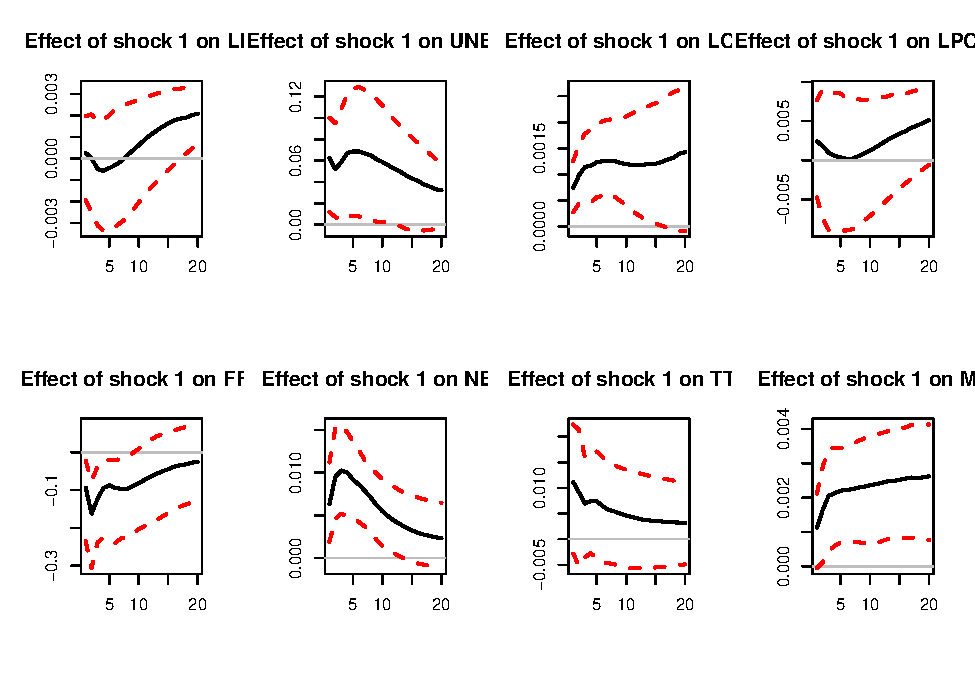
\includegraphics[width=0.95\linewidth]{AdvECTS_files/figure-latex/signrestr1-1} \caption{IRF associated with a monetary policy shock; sign-restriction approach.}\label{fig:signrestr1}
\end{figure}

\begin{Shaded}
\begin{Highlighting}[]
\NormalTok{nb.rotations }\OtherTok{\textless{}{-}}\NormalTok{ res.svar.signs}\SpecialCharTok{$}\NormalTok{xx}
\end{Highlighting}
\end{Shaded}

A remarkable characteristic of sign restrictions is that it does not lead to a unique IRF. In that sense, we say that it is set-identified, not point-identified. By drawing the rotation matrices (\(Q\)) from a distribution and taking the median, we adopt an agnostic approach: ``pure sign restriction approach''.

An alternative approach is the so-called \textbf{penalty-function approach} (PFA, \citet{Uhlig_2005}, present in \citet{Danne_2015}'s package). This approach relies on a \emph{penalty function}:
\[
\begin{array}{llll}f(x)&=&x&\text{ if }x\le0\\
&&100.x&\text{ if }x>0\end{array}
\]
which penalizes positive responses and rewards negative responses.

Let \(\psi_k^j(q)\) be the impulse response of variable \(j\). The \(\psi_k^j(q)\)'s are the elements of \(\psi_k(q)=\Psi_kq\).

Let \(\sigma_j\) be the standard deviation of variable \(j\). Let \(\iota_{j,k}=1\) if we restrict the response of variable \(j\) at the \(k^th\) horizon to be negative, \(\iota_{j,k}=-1\) if we restrict it to be positive, and \(\iota_{j,k}=0\) if there is no restriction. The total penalty is given by \[
\mathbf{P}(q)=\sum_{j=1}^m\sum_{k=0}^Kf\left(\iota_{j,k}\frac{\psi_k^j(q)}{\sigma_j}\right).
\]

We are looking for a solution to
\[\begin{array}{ll}&\min_q \mathbf{P}(q)\\
&\\
\text{s.t. }&q'q=1\end{array}\]

The problem is solved numerically.

\hypertarget{forecast-error-variance-maximization}{%
\subsection{Forecast error variance maximization}\label{forecast-error-variance-maximization}}

The approach presented in this section exploits the derivations of \citet{Uhlig_2004}. \citet{BARSKY2011273} exploit this approach to identify a TFP news shock, that they define as the shock (a) that is orthogonal to the innovation in current utilization-adjusted TFP and (b) that best explains variation in future TFP.

Consider a process \(\{y_t\}\) that admits the infinite MA representation of Eq. \eqref{eq:InfMA}. Let \(Q\) be an orthogonal matrix, an alternative decomposition is:
\begin{eqnarray}
y_t&=&\sum_{h=0}^{+\infty}\Psi_h\underbrace{\eta_{t-h}}_{Q\tilde \eta_{t-h}} = \sum_{h=0}^{+\infty}\underbrace{\Psi_hQ}_{\tilde\Psi_h}\tilde
\eta_{t-h} = \sum_{h=0}^{+\infty}\tilde\Psi_h\tilde \eta_{t-h},
\end{eqnarray}
where \(\tilde \eta_{t-h}=Q'\eta_{t-h}\) are the white-noise shocks associated with the new MA representation. (They also satisfy \(\mathbb{V}ar(\tilde\eta_t)=Id\).)

The \(h\)-step ahead prediction error of \(y_{t+h}\), given all the data up to and including \(t-1\) is given by
\[
e_{t+h}(h)=y_{t+h}-\mathbb{E}_{t-1}(y_{t+h})=\sum_{j=0}^h\tilde \Psi_h\tilde \eta_{t+h-j}.
\]

The variance-covariance matrix of \(e_{t+h}(h)\) is
\[
\Omega(h)=\sum_{j=0}^h\tilde \Psi_j\tilde \Psi_j'=\sum_{j=0}^h \Psi_j \Psi_j'.
\]

We can decompose \(\Omega(h)\) into the contribution of each shock \(l\) (\(l^{th}\) component of \(\tilde{\eta}_t\)):
\[
\Omega^{(h)}=\sum_{l=1}^n\Omega_l^{(h)}(Q)
\]
with
\[
\Omega_l^{(h)}(Q) =\sum_{j=0}^h(\Psi_jq_l)(\Psi_jq_l)',
\]
where \(q_l\) is the \(l^{th}\) column of \(Q\).

This decomposition can be used with the objective of finding the \textbf{impulse vector} \(b\) that is s.t. that it explains as much as possible of the sum of the \(h\)-step ahead prediction error variance of some variable \(i\), say, for prediction horizons \(h \in [\underline{h} , \overline{h}]\).

Formally, the task is to explain as much as possible of the variance
\[
\sigma^2(\underline{h},\overline{h},q_1)=\sum_{h=\underline{h}}^{\overline{h}} \sum_{j=0}^h\left[(\Psi_jq_1)(\Psi_jq_1)'\right]_{i,i}
\]
with a single impulse vector \(q_1\).

Denote by \(E_{ii}\) the matrix that is filled with zeros, except for its (\(i,i\)) entry, set to 1. We have:
\begin{eqnarray*}
\sigma^2(\underline{h},\overline{h},q_1)&=&\sum_{h=\underline{h}}^{\overline{h}} \sum_{j=0}^h\left[(\Psi_jq_1)(\Psi_jq_1)'\right]_{i,i}=\sum_{h=\underline{h}}^{\overline{h}} \sum_{j=0}^h Tr\left[E_{ii}(\Psi_jq_1)(\Psi_jq_1)'\right]\\
&=&\sum_{h=\underline{h}}^{\overline{h}} \sum_{j=0}^h Tr\left[q_1'\Psi_j'E_{ii}\Psi_j q_1\right]\\
&=& q_1'Sq_1,
\end{eqnarray*}
where
\begin{eqnarray*}
\begin{array}{lll}S&=&\sum_{h=\underline{h}}^{\overline{h}}\sum_{j=0}^{h}\Psi_j'E_{ii}\Psi_j\\
&=&\sum_{j=0}^{\overline{h}}(\overline{h}+1-max(\underline{h},j))\Psi_j'E_{ii}\Psi_j\\
&=&\sum_{j=0}^{\overline{h}}(\overline{h}+1-max(\underline{h},j))\Psi_{j,i}'\Psi_{j,i}\\
\end{array}
\end{eqnarray*}
where \(\Psi_{j,i}\) denotes row \(i\) of \(\Psi_{j}\), i.e., the response of variable \(i\) at horizon \(j\) (when \(Q=Id\)).

The maximization problem subject to the side constraint \(q_1'q_1=1\) can be written as a Lagrangian: \[
L=q_1'Sq_1-\lambda(q_1'q_1-1),
\]
with the first-order condition \(Sq_1=\lambda q_1\) (the side constraint is \(q_1'q_1=1\)). From this equation, we see that the solution \(q_1\) is an eigenvector of \(S\), the one associated with eigenvalue \(\lambda\). We also see that \(\sigma^2(\underline{h},\overline{h},q_1)=\lambda\). Thus, to maximize this variance, we need to find the eigenvector of \(S\) that is associated with the maximal eigenvalue \(\lambda\). That defines the first principal component (see XXXXXXX). That is, if \(S\) admits the following spectral decomposition:
\[
S = \mathcal{P}D\mathcal{P}',
\]
where \(D\) is diagonal matrix whose entries are the (ordered) eigenvalues: \(\lambda_1 \ge \lambda_2 \ge \dots \ge \lambda_n \ge 0\), then \(\sigma^2(\underline{h},\overline{h},q_1)\) is maximized for \(q_1 = p_1\), where \(p_1\) is the first column of \(\mathcal{P}\).

\hypertarget{NonGaussian}{%
\subsection{Identificagtion based on non-normality of the shocks}\label{NonGaussian}}

In this section, we show that the non-identification of the structural shocks (\(\eta_t\)) is very specific to the Gaussian case. We propose consistent estimation approaches in the context of non-Gaussian shocks. In a first part, we focus on non-Gaussian SVAR models; in a second part, we discuss the case of non-Gaussian SVARMA models.

\textbf{Non-Gaussian SVAR models}

The estimation of (S)VARs is more common than that of (S)VARMAs. (Simpler estimation of \(\Phi_k\)'s). We have seen in what precedes that, in the Gaussian case, we cannot identify \(B\) in the Gaussian case. That is, even if we observe an infinite number of i.i.d. \(B \eta_t\), we cannot recover \(B\) is the \(\eta_t\)'s are Gaussian. Indeed, if \(\eta_t \sim \mathcal{N}(0,Id)\), then the distribution of \(\varepsilon_t \equiv B \eta_t\) is \(\mathcal{N}(0,BB')\).

Hence \(\Omega = B B'\) is observed (in the population), but for any orthogonal matrix \(Q\) (i.e.~\(QQ'=Id\)), we also have \(BQ \eta_t \sim \mathcal{N}(0,\Omega)\).

Example: Bivariate Gaussian case (Eq. \eqref{eq:VARMA111}, with \(\Theta_1=0\))

\(\left[\begin{array}{c}\eta_{1,t}\\ \eta_{2,t}\end{array}\right]\sim \mathcal{N}(0,Id)\),
\(B = \left[\begin{array}{cc} 1 & 2 \\ -1 & 1 \end{array}\right]\) and
\(Q = \left[\begin{array}{cc} \cos(\pi/3) & -\sin(\pi/3) \\ \sin(\pi/3) & \cos(\pi/3) \end{array}\right]\) (rotation).

\(\Rightarrow\) Distribution of \(B \eta_t\) versus that of \(BQ\eta_t\)?

\begin{Shaded}
\begin{Highlighting}[]
\NormalTok{theta.angle }\OtherTok{\textless{}{-}}\NormalTok{ pi}\SpecialCharTok{/}\DecValTok{3}
\NormalTok{Q }\OtherTok{\textless{}{-}} \FunctionTok{matrix}\NormalTok{(}\FunctionTok{c}\NormalTok{(}\FunctionTok{cos}\NormalTok{(theta.angle),}\FunctionTok{sin}\NormalTok{(theta.angle),}\SpecialCharTok{{-}}\FunctionTok{sin}\NormalTok{(theta.angle),}\FunctionTok{cos}\NormalTok{(theta.angle)),}\DecValTok{2}\NormalTok{,}\DecValTok{2}\NormalTok{)}
\CommentTok{\#nb.sim \textless{}{-} 10\^{}4}
\NormalTok{nb.sim }\OtherTok{\textless{}{-}} \DecValTok{10}\SpecialCharTok{\^{}}\DecValTok{2}
\NormalTok{distri}\FloatTok{.1} \OtherTok{\textless{}{-}} \FunctionTok{list}\NormalTok{(}\AttributeTok{type=}\FunctionTok{c}\NormalTok{(}\StringTok{"gaussian"}\NormalTok{),}\AttributeTok{name=}\StringTok{"Panel (a) Gaussian"}\NormalTok{,}\AttributeTok{name.4.table=}\StringTok{"Gaussian"}\NormalTok{)}
\NormalTok{distri}\FloatTok{.2} \OtherTok{\textless{}{-}} \FunctionTok{list}\NormalTok{(}\AttributeTok{type=}\FunctionTok{c}\NormalTok{(}\StringTok{"mixt.gaussian"}\NormalTok{),}\AttributeTok{mu=}\DecValTok{0}\NormalTok{,}\AttributeTok{sigma=}\DecValTok{5}\NormalTok{,}\AttributeTok{p=}\NormalTok{.}\DecValTok{03}\NormalTok{,}\AttributeTok{name=}\StringTok{"Panel (b) Mixture of Gaussian"}\NormalTok{,}\AttributeTok{name.4.table=}\StringTok{"Mixture of Gaussian"}\NormalTok{)}
\NormalTok{distri}\FloatTok{.3} \OtherTok{\textless{}{-}} \FunctionTok{list}\NormalTok{(}\AttributeTok{type=}\FunctionTok{c}\NormalTok{(}\StringTok{"student"}\NormalTok{),}\AttributeTok{df=}\FunctionTok{c}\NormalTok{(}\DecValTok{5}\NormalTok{),}\AttributeTok{name=}\StringTok{"Panel (c) Student (df: 5)"}\NormalTok{,}\AttributeTok{name.4.table=}\StringTok{"Student (df: 5)"}\NormalTok{)}
\NormalTok{distri}\FloatTok{.4} \OtherTok{\textless{}{-}} \FunctionTok{list}\NormalTok{(}\AttributeTok{type=}\FunctionTok{c}\NormalTok{(}\StringTok{"student"}\NormalTok{),}\AttributeTok{df=}\FunctionTok{c}\NormalTok{(}\DecValTok{10}\NormalTok{),}\AttributeTok{name=}\StringTok{"Panel (d) Student (df: 10)"}\NormalTok{,}\AttributeTok{name.4.table=}\StringTok{"Student (df: 10)"}\NormalTok{)}
\NormalTok{x.lim }\OtherTok{\textless{}{-}} \FunctionTok{c}\NormalTok{(}\SpecialCharTok{{-}}\DecValTok{7}\NormalTok{,}\DecValTok{7}\NormalTok{)}
\NormalTok{y.lim }\OtherTok{\textless{}{-}} \FunctionTok{c}\NormalTok{(}\SpecialCharTok{{-}}\DecValTok{5}\NormalTok{,}\DecValTok{5}\NormalTok{)}
\NormalTok{nb.points }\OtherTok{\textless{}{-}} \DecValTok{100}
\NormalTok{x.points }\OtherTok{\textless{}{-}} \FunctionTok{seq}\NormalTok{(x.lim[}\DecValTok{1}\NormalTok{],x.lim[}\DecValTok{2}\NormalTok{],}\AttributeTok{length.out=}\NormalTok{nb.points)}
\NormalTok{y.points }\OtherTok{\textless{}{-}}\NormalTok{ x.points}
\NormalTok{all.x }\OtherTok{\textless{}{-}} \FunctionTok{c}\NormalTok{(}\FunctionTok{matrix}\NormalTok{(x.points,nb.points,nb.points))}
\NormalTok{all.y }\OtherTok{\textless{}{-}} \FunctionTok{c}\NormalTok{(}\FunctionTok{t}\NormalTok{(}\FunctionTok{matrix}\NormalTok{(x.points,nb.points,nb.points)))}
\NormalTok{eps }\OtherTok{\textless{}{-}} \FunctionTok{cbind}\NormalTok{(all.x,all.y)}
\FunctionTok{par}\NormalTok{(}\AttributeTok{plt=}\FunctionTok{c}\NormalTok{(.}\DecValTok{25}\NormalTok{,.}\DecValTok{9}\NormalTok{,.}\DecValTok{25}\NormalTok{,.}\DecValTok{8}\NormalTok{))}
\NormalTok{eta}\FloatTok{.1} \OtherTok{\textless{}{-}} \FunctionTok{simul.distri}\NormalTok{(distri}\FloatTok{.1}\NormalTok{,nb.sim)}
\NormalTok{eta}\FloatTok{.2} \OtherTok{\textless{}{-}} \FunctionTok{simul.distri}\NormalTok{(distri}\FloatTok{.1}\NormalTok{,nb.sim)}
\NormalTok{epsilon.C }\OtherTok{\textless{}{-}} \FunctionTok{cbind}\NormalTok{(eta}\FloatTok{.1}\NormalTok{,eta}\FloatTok{.2}\NormalTok{) }\SpecialCharTok{\%*\%} \FunctionTok{t}\NormalTok{(C)}
\NormalTok{epsilon.CQ }\OtherTok{\textless{}{-}} \FunctionTok{cbind}\NormalTok{(eta}\FloatTok{.1}\NormalTok{,eta}\FloatTok{.2}\NormalTok{) }\SpecialCharTok{\%*\%} \FunctionTok{t}\NormalTok{(C }\SpecialCharTok{\%*\%}\NormalTok{ Q)}
\NormalTok{Model}\SpecialCharTok{$}\NormalTok{distri }\OtherTok{\textless{}{-}} \FunctionTok{list}\NormalTok{(}\AttributeTok{type=}\FunctionTok{c}\NormalTok{(}\StringTok{"gaussian"}\NormalTok{,}\StringTok{"gaussian"}\NormalTok{),}\AttributeTok{df=}\FunctionTok{c}\NormalTok{(}\ConstantTok{NaN}\NormalTok{,}\ConstantTok{NaN}\NormalTok{))}
\FunctionTok{par}\NormalTok{(}\AttributeTok{mfrow=}\FunctionTok{c}\NormalTok{(}\DecValTok{1}\NormalTok{,}\DecValTok{2}\NormalTok{))}
\FunctionTok{plot}\NormalTok{(epsilon.C[,}\DecValTok{1}\NormalTok{],epsilon.C[,}\DecValTok{2}\NormalTok{],}\AttributeTok{pch=}\DecValTok{19}\NormalTok{,}
     \AttributeTok{xlim=}\NormalTok{x.lim,}\AttributeTok{ylim=}\NormalTok{y.lim,}\AttributeTok{col=}\StringTok{"\#00000044"}\NormalTok{,}
     \AttributeTok{xlab=}\FunctionTok{expression}\NormalTok{(epsilon[}\DecValTok{1}\NormalTok{]),}
     \AttributeTok{ylab=}\FunctionTok{expression}\NormalTok{(epsilon[}\DecValTok{2}\NormalTok{]),}\AttributeTok{cex.lab=}\FloatTok{1.6}\NormalTok{,}\AttributeTok{cex.main=}\FloatTok{1.6}\NormalTok{,}
     \AttributeTok{main=}\FunctionTok{expression}\NormalTok{(}\FunctionTok{paste}\NormalTok{(}\StringTok{"Distribution of "}\NormalTok{,epsilon[t],}\StringTok{" = "}\NormalTok{,B,eta[t],}\AttributeTok{sep=}\StringTok{""}\NormalTok{)))}
\NormalTok{z }\OtherTok{\textless{}{-}} \FunctionTok{matrix}\NormalTok{(}\FunctionTok{exp}\NormalTok{(}\FunctionTok{g}\NormalTok{(eps,Model)),nb.points,nb.points)}
\FunctionTok{par}\NormalTok{(}\AttributeTok{new=}\ConstantTok{TRUE}\NormalTok{)}
\NormalTok{max.z }\OtherTok{\textless{}{-}} \FunctionTok{max}\NormalTok{(z)}
\NormalTok{levels }\OtherTok{\textless{}{-}} \FunctionTok{c}\NormalTok{(.}\DecValTok{01}\NormalTok{,.}\DecValTok{1}\NormalTok{,.}\DecValTok{3}\NormalTok{,.}\DecValTok{6}\NormalTok{,.}\DecValTok{9}\NormalTok{)}\SpecialCharTok{*}\NormalTok{max.z}
\FunctionTok{contour}\NormalTok{(x.points,y.points,z,}\AttributeTok{levels=}\NormalTok{levels,}\AttributeTok{xlim=}\NormalTok{x.lim,}\AttributeTok{ylim=}\NormalTok{y.lim,}\AttributeTok{col=}\StringTok{"red"}\NormalTok{,}\AttributeTok{lwd=}\DecValTok{2}\NormalTok{)}
\FunctionTok{plot}\NormalTok{(epsilon.CQ[,}\DecValTok{1}\NormalTok{],epsilon.CQ[,}\DecValTok{2}\NormalTok{],}\AttributeTok{pch=}\DecValTok{19}\NormalTok{,}
     \AttributeTok{xlim=}\NormalTok{x.lim,}\AttributeTok{ylim=}\NormalTok{y.lim,}\AttributeTok{col=}\StringTok{"\#00000044"}\NormalTok{,}
     \AttributeTok{xlab=}\FunctionTok{expression}\NormalTok{(epsilon[}\DecValTok{1}\NormalTok{]),}
     \AttributeTok{ylab=}\FunctionTok{expression}\NormalTok{(epsilon[}\DecValTok{2}\NormalTok{]),}\AttributeTok{cex.lab=}\FloatTok{1.6}\NormalTok{,}\AttributeTok{cex.main=}\FloatTok{1.6}\NormalTok{,}
     \AttributeTok{main=}\FunctionTok{expression}\NormalTok{(}\FunctionTok{paste}\NormalTok{(}\StringTok{"Distribution of "}\NormalTok{,epsilon[t],}\StringTok{" = "}\NormalTok{,BQ,eta[t],}\AttributeTok{sep=}\StringTok{""}\NormalTok{)))}
\NormalTok{z }\OtherTok{\textless{}{-}} \FunctionTok{matrix}\NormalTok{(}\FunctionTok{exp}\NormalTok{(}\FunctionTok{g}\NormalTok{(eps,Model)),nb.points,nb.points)}
\FunctionTok{par}\NormalTok{(}\AttributeTok{new=}\ConstantTok{TRUE}\NormalTok{)}
\NormalTok{max.z }\OtherTok{\textless{}{-}} \FunctionTok{max}\NormalTok{(z)}
\NormalTok{levels }\OtherTok{\textless{}{-}} \FunctionTok{c}\NormalTok{(.}\DecValTok{01}\NormalTok{,.}\DecValTok{1}\NormalTok{,.}\DecValTok{3}\NormalTok{,.}\DecValTok{6}\NormalTok{,.}\DecValTok{9}\NormalTok{)}\SpecialCharTok{*}\NormalTok{max.z}
\FunctionTok{contour}\NormalTok{(x.points,y.points,z,}\AttributeTok{levels=}\NormalTok{levels,}\AttributeTok{xlim=}\NormalTok{x.lim,}\AttributeTok{ylim=}\NormalTok{y.lim,}\AttributeTok{col=}\StringTok{"red"}\NormalTok{,}\AttributeTok{lwd=}\DecValTok{2}\NormalTok{)}
\end{Highlighting}
\end{Shaded}

\begin{figure}
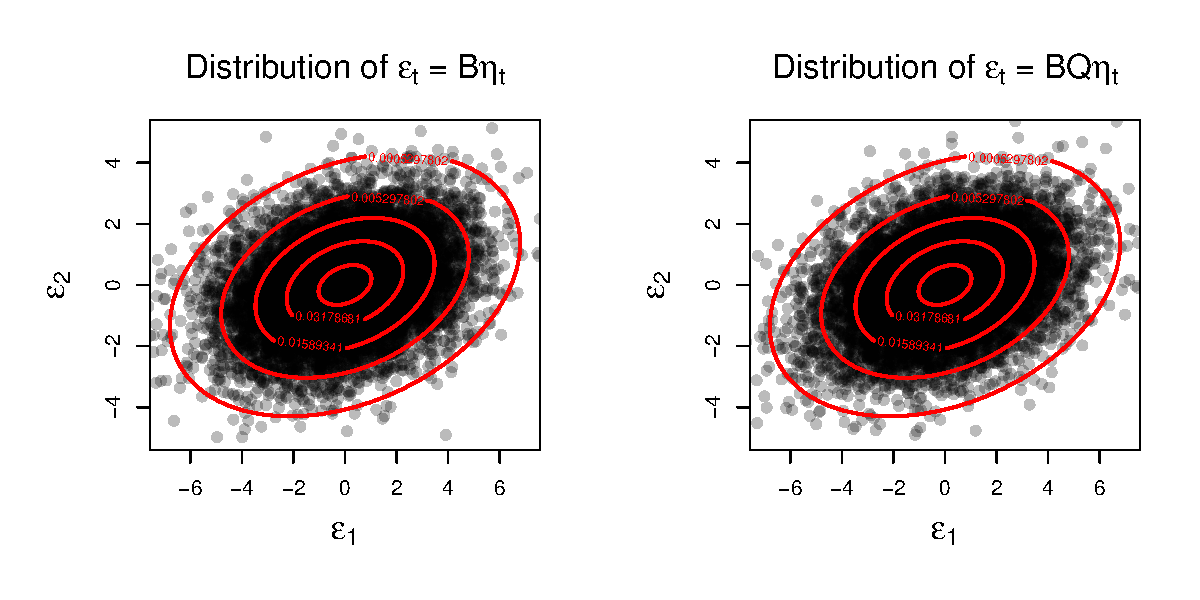
\includegraphics[width=0.95\linewidth]{images/Figure_A} \caption{XXXX.}\label{fig:preMadeFigureICA}
\end{figure}

\begin{figure}
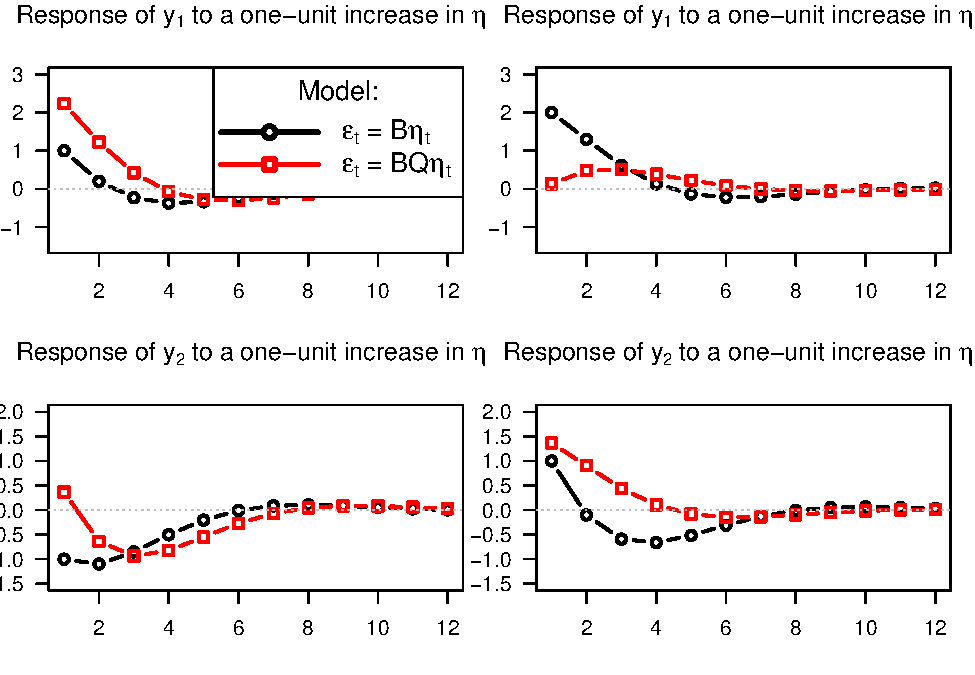
\includegraphics[width=0.95\linewidth]{AdvECTS_files/figure-latex/preMadeFigureICA2-1} \caption{XXXX.}\label{fig:preMadeFigureICA2}
\end{figure}

External restrictions (economic hypotheses) are needed to identify \(B\) (see previous sections). But such restrictions may not be necessary if the structural shocks are not Gaussian.

That is, the identification problem is very specific to normally-distributed \(\eta_t\)'s.

\href{https://www.mitpressjournals.org/doi/abs/10.1162/003465303772815727?journalCode=rest}{Rigobon (2003)}
\href{https://www.sciencedirect.com/science/article/abs/pii/S0304393204000698}{Normandin and Phaneuf (2004)}
\href{https://onlinelibrary.wiley.com/doi/abs/10.1111/j.1538-4616.2008.00151.x}{Lanne and Lutkepohl (2008)}

Example: Bivariate Gaussian + Student (5) case:

\(\eta_{1,t} \sim \mathcal{N}(0,1)\), \(\eta_{2,t} \sim t(5)\),
\(B = \left[\begin{array}{cc} 1 & 2 \\ -1 & 1 \end{array}\right]\) and
\(Q = \left[\begin{array}{cc} \cos(\pi/3) & -\sin(\pi/3) \\ \sin(\pi/3) & \cos(\pi/3) \end{array}\right]\).

Distribution of \(B \eta_t\) versus that of \(BQ\eta_t\)?

\begin{Shaded}
\begin{Highlighting}[]
\NormalTok{theta.angle }\OtherTok{\textless{}{-}}\NormalTok{ pi}\SpecialCharTok{/}\DecValTok{3}
\NormalTok{Q }\OtherTok{\textless{}{-}} \FunctionTok{matrix}\NormalTok{(}\FunctionTok{c}\NormalTok{(}\FunctionTok{cos}\NormalTok{(theta.angle),}\FunctionTok{sin}\NormalTok{(theta.angle),}\SpecialCharTok{{-}}\FunctionTok{sin}\NormalTok{(theta.angle),}\FunctionTok{cos}\NormalTok{(theta.angle)),}\DecValTok{2}\NormalTok{,}\DecValTok{2}\NormalTok{)}
\CommentTok{\#nb.sim \textless{}{-} 10\^{}4}
\NormalTok{nb.sim }\OtherTok{\textless{}{-}} \DecValTok{10}\SpecialCharTok{\^{}}\DecValTok{2}
\NormalTok{distri}\FloatTok{.1} \OtherTok{\textless{}{-}} \FunctionTok{list}\NormalTok{(}\AttributeTok{type=}\FunctionTok{c}\NormalTok{(}\StringTok{"gaussian"}\NormalTok{),}\AttributeTok{name=}\StringTok{"Panel (a) Gaussian"}\NormalTok{,}\AttributeTok{name.4.table=}\StringTok{"Gaussian"}\NormalTok{)}
\NormalTok{distri}\FloatTok{.2} \OtherTok{\textless{}{-}} \FunctionTok{list}\NormalTok{(}\AttributeTok{type=}\FunctionTok{c}\NormalTok{(}\StringTok{"mixt.gaussian"}\NormalTok{),}\AttributeTok{mu=}\DecValTok{0}\NormalTok{,}\AttributeTok{sigma=}\DecValTok{5}\NormalTok{,}\AttributeTok{p=}\NormalTok{.}\DecValTok{03}\NormalTok{,}\AttributeTok{name=}\StringTok{"Panel (b) Mixture of Gaussian"}\NormalTok{,}\AttributeTok{name.4.table=}\StringTok{"Mixture of Gaussian"}\NormalTok{)}
\NormalTok{distri}\FloatTok{.3} \OtherTok{\textless{}{-}} \FunctionTok{list}\NormalTok{(}\AttributeTok{type=}\FunctionTok{c}\NormalTok{(}\StringTok{"student"}\NormalTok{),}\AttributeTok{df=}\FunctionTok{c}\NormalTok{(}\DecValTok{5}\NormalTok{),}\AttributeTok{name=}\StringTok{"Panel (c) Student (df: 5)"}\NormalTok{,}\AttributeTok{name.4.table=}\StringTok{"Student (df: 5)"}\NormalTok{)}
\NormalTok{distri}\FloatTok{.4} \OtherTok{\textless{}{-}} \FunctionTok{list}\NormalTok{(}\AttributeTok{type=}\FunctionTok{c}\NormalTok{(}\StringTok{"student"}\NormalTok{),}\AttributeTok{df=}\FunctionTok{c}\NormalTok{(}\DecValTok{10}\NormalTok{),}\AttributeTok{name=}\StringTok{"Panel (d) Student (df: 10)"}\NormalTok{,}\AttributeTok{name.4.table=}\StringTok{"Student (df: 10)"}\NormalTok{)}
\NormalTok{x.lim }\OtherTok{\textless{}{-}} \FunctionTok{c}\NormalTok{(}\SpecialCharTok{{-}}\DecValTok{7}\NormalTok{,}\DecValTok{7}\NormalTok{)}
\NormalTok{y.lim }\OtherTok{\textless{}{-}} \FunctionTok{c}\NormalTok{(}\SpecialCharTok{{-}}\DecValTok{5}\NormalTok{,}\DecValTok{5}\NormalTok{)}
\NormalTok{nb.points }\OtherTok{\textless{}{-}} \DecValTok{100}
\NormalTok{x.points }\OtherTok{\textless{}{-}} \FunctionTok{seq}\NormalTok{(x.lim[}\DecValTok{1}\NormalTok{],x.lim[}\DecValTok{2}\NormalTok{],}\AttributeTok{length.out=}\NormalTok{nb.points)}
\NormalTok{y.points }\OtherTok{\textless{}{-}}\NormalTok{ x.points}
\NormalTok{all.x }\OtherTok{\textless{}{-}} \FunctionTok{c}\NormalTok{(}\FunctionTok{matrix}\NormalTok{(x.points,nb.points,nb.points))}
\NormalTok{all.y }\OtherTok{\textless{}{-}} \FunctionTok{c}\NormalTok{(}\FunctionTok{t}\NormalTok{(}\FunctionTok{matrix}\NormalTok{(x.points,nb.points,nb.points)))}
\NormalTok{eps }\OtherTok{\textless{}{-}} \FunctionTok{cbind}\NormalTok{(all.x,all.y)}
\FunctionTok{par}\NormalTok{(}\AttributeTok{plt=}\FunctionTok{c}\NormalTok{(.}\DecValTok{25}\NormalTok{,.}\DecValTok{9}\NormalTok{,.}\DecValTok{25}\NormalTok{,.}\DecValTok{8}\NormalTok{))}
\NormalTok{eta}\FloatTok{.1} \OtherTok{\textless{}{-}} \FunctionTok{simul.distri}\NormalTok{(distri}\FloatTok{.1}\NormalTok{,nb.sim)}
\NormalTok{eta}\FloatTok{.2} \OtherTok{\textless{}{-}} \FunctionTok{simul.distri}\NormalTok{(distri}\FloatTok{.3}\NormalTok{,nb.sim)}
\NormalTok{epsilon.C }\OtherTok{\textless{}{-}} \FunctionTok{cbind}\NormalTok{(eta}\FloatTok{.1}\NormalTok{,eta}\FloatTok{.2}\NormalTok{) }\SpecialCharTok{\%*\%} \FunctionTok{t}\NormalTok{(C)}
\NormalTok{epsilon.CQ }\OtherTok{\textless{}{-}} \FunctionTok{cbind}\NormalTok{(eta}\FloatTok{.1}\NormalTok{,eta}\FloatTok{.2}\NormalTok{) }\SpecialCharTok{\%*\%} \FunctionTok{t}\NormalTok{(C }\SpecialCharTok{\%*\%}\NormalTok{ Q)}
\NormalTok{Model}\SpecialCharTok{$}\NormalTok{distri }\OtherTok{\textless{}{-}} \FunctionTok{list}\NormalTok{(}\AttributeTok{type=}\FunctionTok{c}\NormalTok{(}\StringTok{"gaussian"}\NormalTok{,}\StringTok{"student"}\NormalTok{),}\AttributeTok{df=}\FunctionTok{c}\NormalTok{(}\ConstantTok{NaN}\NormalTok{,}\DecValTok{5}\NormalTok{))}
\FunctionTok{par}\NormalTok{(}\AttributeTok{mfrow=}\FunctionTok{c}\NormalTok{(}\DecValTok{1}\NormalTok{,}\DecValTok{2}\NormalTok{))}
\FunctionTok{plot}\NormalTok{(epsilon.C[,}\DecValTok{1}\NormalTok{],epsilon.C[,}\DecValTok{2}\NormalTok{],}\AttributeTok{pch=}\DecValTok{19}\NormalTok{,}
     \AttributeTok{xlim=}\NormalTok{x.lim,}\AttributeTok{ylim=}\NormalTok{y.lim,}\AttributeTok{col=}\StringTok{"\#00000044"}\NormalTok{,}
     \AttributeTok{xlab=}\FunctionTok{expression}\NormalTok{(epsilon[}\DecValTok{1}\NormalTok{]),}
     \AttributeTok{ylab=}\FunctionTok{expression}\NormalTok{(epsilon[}\DecValTok{2}\NormalTok{]),}\AttributeTok{cex.lab=}\FloatTok{1.6}\NormalTok{,}\AttributeTok{cex.main=}\FloatTok{1.6}\NormalTok{,}
     \AttributeTok{main=}\FunctionTok{expression}\NormalTok{(}\FunctionTok{paste}\NormalTok{(}\StringTok{"Distribution of "}\NormalTok{,epsilon[t],}\StringTok{" = "}\NormalTok{,B,eta[t],}\AttributeTok{sep=}\StringTok{""}\NormalTok{)))}
\NormalTok{z }\OtherTok{\textless{}{-}} \FunctionTok{matrix}\NormalTok{(}\FunctionTok{exp}\NormalTok{(}\FunctionTok{g}\NormalTok{(eps,Model)),nb.points,nb.points)}
\FunctionTok{par}\NormalTok{(}\AttributeTok{new=}\ConstantTok{TRUE}\NormalTok{)}
\NormalTok{max.z }\OtherTok{\textless{}{-}} \FunctionTok{max}\NormalTok{(z)}
\NormalTok{levels }\OtherTok{\textless{}{-}} \FunctionTok{c}\NormalTok{(.}\DecValTok{01}\NormalTok{,.}\DecValTok{1}\NormalTok{,.}\DecValTok{3}\NormalTok{,.}\DecValTok{6}\NormalTok{,.}\DecValTok{9}\NormalTok{)}\SpecialCharTok{*}\NormalTok{max.z}
\FunctionTok{contour}\NormalTok{(x.points,y.points,z,}\AttributeTok{levels=}\NormalTok{levels,}\AttributeTok{xlim=}\NormalTok{x.lim,}\AttributeTok{ylim=}\NormalTok{y.lim,}\AttributeTok{col=}\StringTok{"red"}\NormalTok{,}\AttributeTok{lwd=}\DecValTok{2}\NormalTok{)}
\FunctionTok{plot}\NormalTok{(epsilon.CQ[,}\DecValTok{1}\NormalTok{],epsilon.CQ[,}\DecValTok{2}\NormalTok{],}\AttributeTok{pch=}\DecValTok{19}\NormalTok{,}
     \AttributeTok{xlim=}\NormalTok{x.lim,}\AttributeTok{ylim=}\NormalTok{y.lim,}\AttributeTok{col=}\StringTok{"\#00000044"}\NormalTok{,}
     \AttributeTok{xlab=}\FunctionTok{expression}\NormalTok{(epsilon[}\DecValTok{1}\NormalTok{]),}
     \AttributeTok{ylab=}\FunctionTok{expression}\NormalTok{(epsilon[}\DecValTok{2}\NormalTok{]),}\AttributeTok{cex.lab=}\FloatTok{1.6}\NormalTok{,}\AttributeTok{cex.main=}\FloatTok{1.6}\NormalTok{,}
     \AttributeTok{main=}\FunctionTok{expression}\NormalTok{(}\FunctionTok{paste}\NormalTok{(}\StringTok{"Distribution of "}\NormalTok{,epsilon[t],}\StringTok{" = "}\NormalTok{,BQ,eta[t],}\AttributeTok{sep=}\StringTok{""}\NormalTok{)))}
\NormalTok{z }\OtherTok{\textless{}{-}} \FunctionTok{matrix}\NormalTok{(}\FunctionTok{exp}\NormalTok{(}\FunctionTok{g}\NormalTok{(eps,Model)),nb.points,nb.points)}
\FunctionTok{par}\NormalTok{(}\AttributeTok{new=}\ConstantTok{TRUE}\NormalTok{)}
\NormalTok{max.z }\OtherTok{\textless{}{-}} \FunctionTok{max}\NormalTok{(z)}
\NormalTok{levels }\OtherTok{\textless{}{-}} \FunctionTok{c}\NormalTok{(.}\DecValTok{01}\NormalTok{,.}\DecValTok{1}\NormalTok{,.}\DecValTok{3}\NormalTok{,.}\DecValTok{6}\NormalTok{,.}\DecValTok{9}\NormalTok{)}\SpecialCharTok{*}\NormalTok{max.z}
\FunctionTok{contour}\NormalTok{(x.points,y.points,z,}\AttributeTok{levels=}\NormalTok{levels,}\AttributeTok{xlim=}\NormalTok{x.lim,}\AttributeTok{ylim=}\NormalTok{y.lim,}\AttributeTok{col=}\StringTok{"red"}\NormalTok{,}\AttributeTok{lwd=}\DecValTok{2}\NormalTok{)}
\end{Highlighting}
\end{Shaded}

\begin{figure}
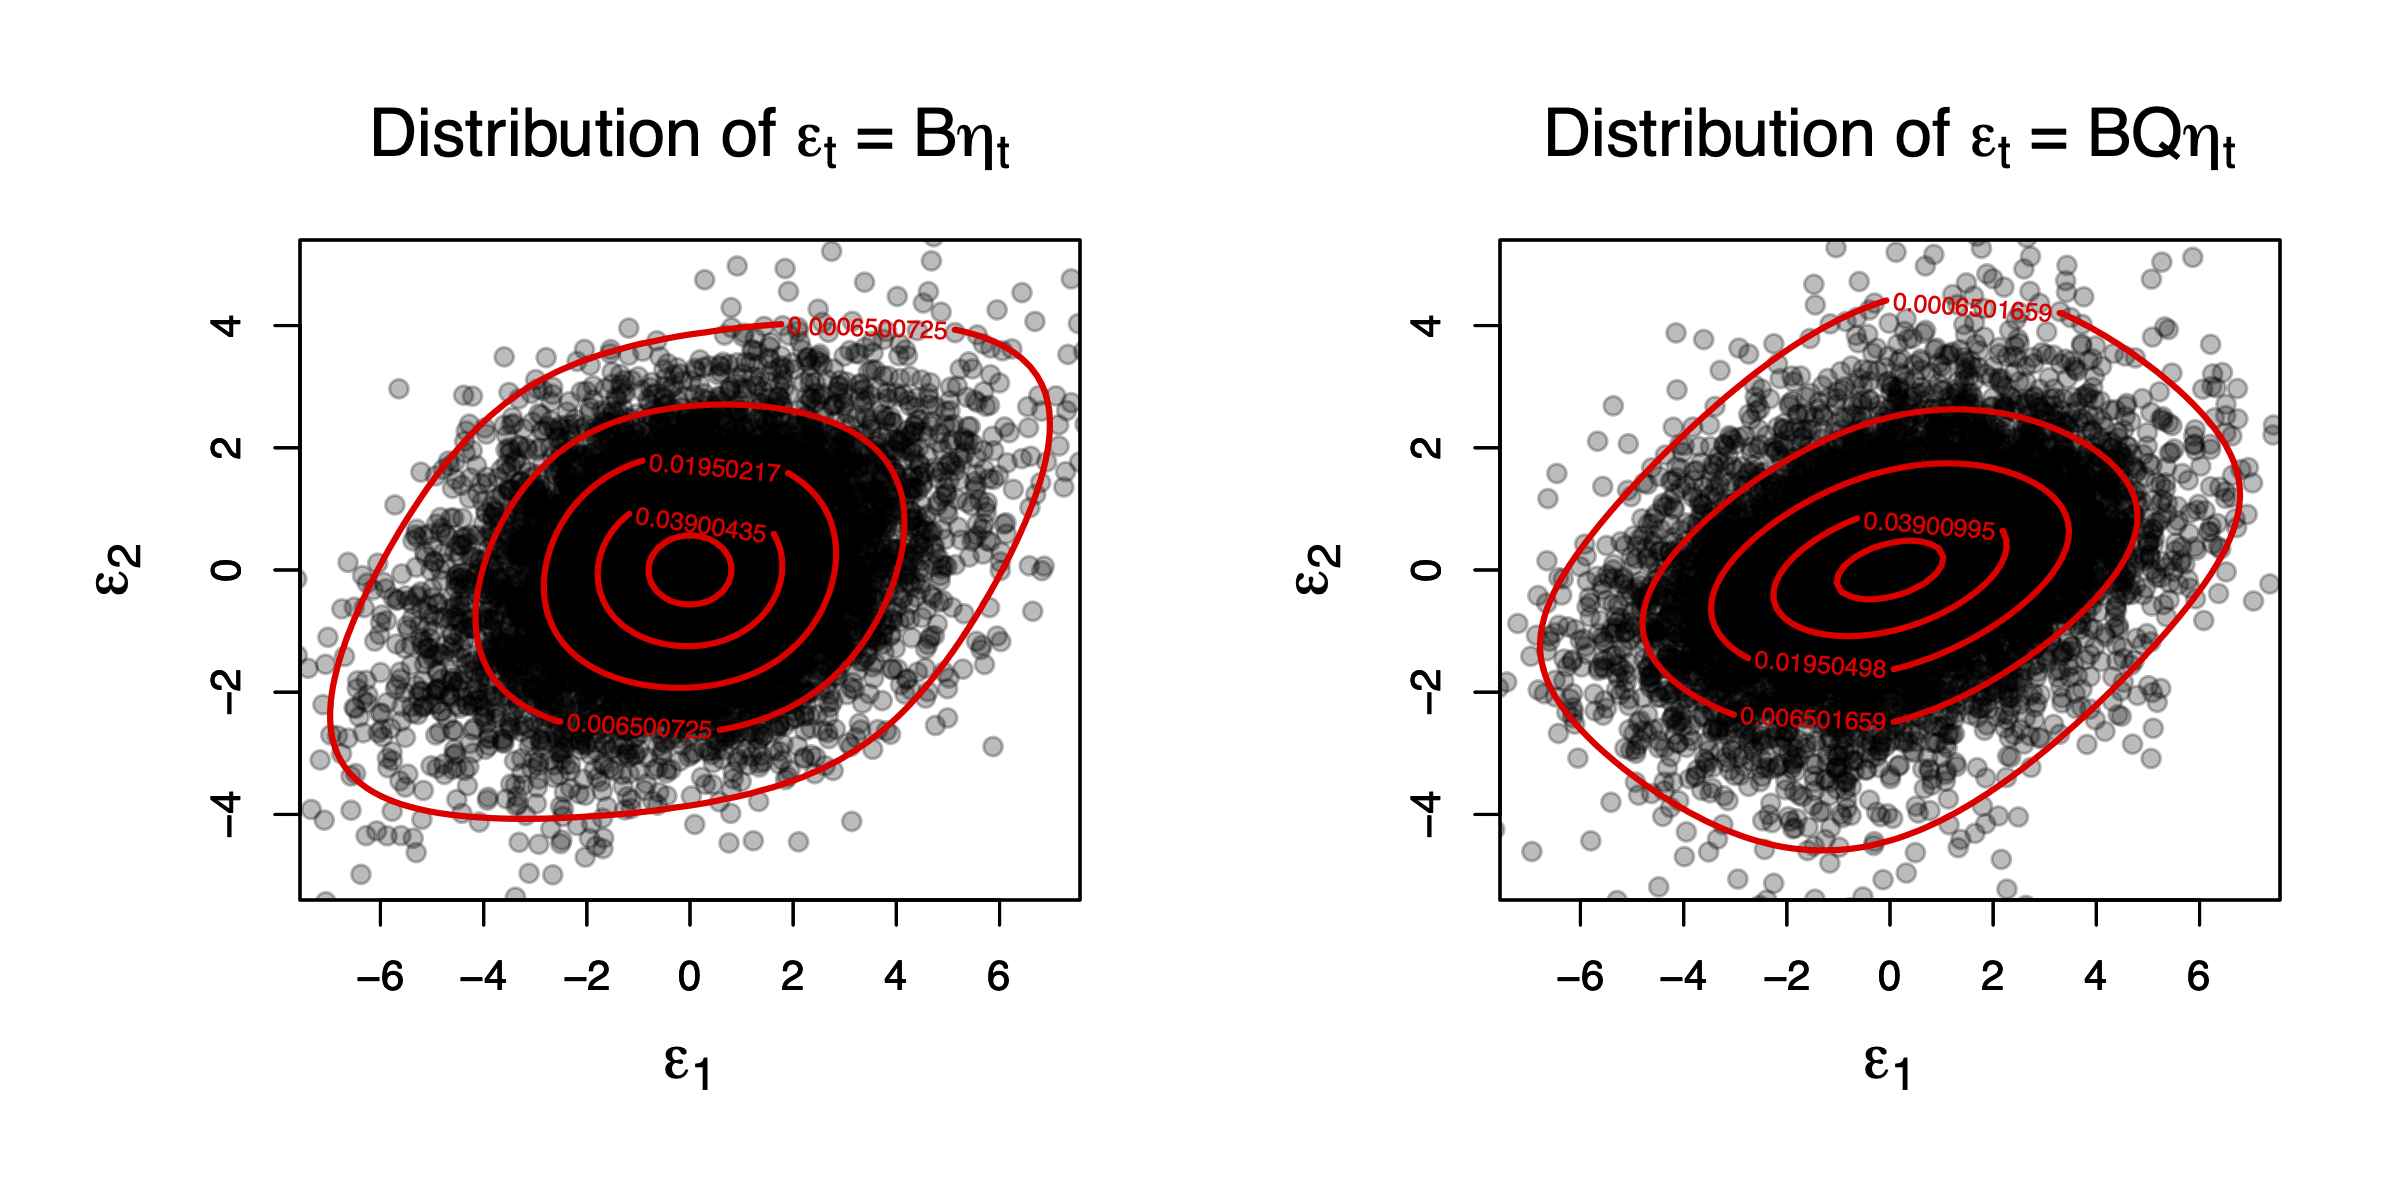
\includegraphics[width=0.95\linewidth]{images/Figure_C} \caption{XXXX.}\label{fig:preMadeFigureICAGaussianStudent}
\end{figure}

NB: In both cases, we have \(\mathbb{V}ar(\varepsilon_t)=BB'\).

Example: Bivariate Student (5) case

\(\eta_{1,t} \sim t(5)\), \(\eta_{2,t} \sim t(5)\),
\(B = \left[\begin{array}{cc} 1 & 2 \\ -1 & 1 \end{array}\right]\) and
\(Q = \left[\begin{array}{cc} \cos(\pi/3) & -\sin(\pi/3) \\ \sin(\pi/3) & \cos(\pi/3) \end{array}\right]\).

\(\Rightarrow\) Distribution of \(B \eta_t\) versus that of \(BQ\eta_t\)?

\begin{Shaded}
\begin{Highlighting}[]
\NormalTok{theta.angle }\OtherTok{\textless{}{-}}\NormalTok{ pi}\SpecialCharTok{/}\DecValTok{3}
\NormalTok{Q }\OtherTok{\textless{}{-}} \FunctionTok{matrix}\NormalTok{(}\FunctionTok{c}\NormalTok{(}\FunctionTok{cos}\NormalTok{(theta.angle),}\FunctionTok{sin}\NormalTok{(theta.angle),}\SpecialCharTok{{-}}\FunctionTok{sin}\NormalTok{(theta.angle),}\FunctionTok{cos}\NormalTok{(theta.angle)),}\DecValTok{2}\NormalTok{,}\DecValTok{2}\NormalTok{)}
\CommentTok{\#nb.sim \textless{}{-} 10\^{}4}
\NormalTok{nb.sim }\OtherTok{\textless{}{-}} \DecValTok{10}\SpecialCharTok{\^{}}\DecValTok{2}
\NormalTok{distri}\FloatTok{.1} \OtherTok{\textless{}{-}} \FunctionTok{list}\NormalTok{(}\AttributeTok{type=}\FunctionTok{c}\NormalTok{(}\StringTok{"gaussian"}\NormalTok{),}\AttributeTok{name=}\StringTok{"Panel (a) Gaussian"}\NormalTok{,}\AttributeTok{name.4.table=}\StringTok{"Gaussian"}\NormalTok{)}
\NormalTok{distri}\FloatTok{.2} \OtherTok{\textless{}{-}} \FunctionTok{list}\NormalTok{(}\AttributeTok{type=}\FunctionTok{c}\NormalTok{(}\StringTok{"mixt.gaussian"}\NormalTok{),}\AttributeTok{mu=}\DecValTok{0}\NormalTok{,}\AttributeTok{sigma=}\DecValTok{5}\NormalTok{,}\AttributeTok{p=}\NormalTok{.}\DecValTok{03}\NormalTok{,}\AttributeTok{name=}\StringTok{"Panel (b) Mixture of Gaussian"}\NormalTok{,}\AttributeTok{name.4.table=}\StringTok{"Mixture of Gaussian"}\NormalTok{)}
\NormalTok{distri}\FloatTok{.3} \OtherTok{\textless{}{-}} \FunctionTok{list}\NormalTok{(}\AttributeTok{type=}\FunctionTok{c}\NormalTok{(}\StringTok{"student"}\NormalTok{),}\AttributeTok{df=}\FunctionTok{c}\NormalTok{(}\DecValTok{5}\NormalTok{),}\AttributeTok{name=}\StringTok{"Panel (c) Student (df: 5)"}\NormalTok{,}\AttributeTok{name.4.table=}\StringTok{"Student (df: 5)"}\NormalTok{)}
\NormalTok{distri}\FloatTok{.4} \OtherTok{\textless{}{-}} \FunctionTok{list}\NormalTok{(}\AttributeTok{type=}\FunctionTok{c}\NormalTok{(}\StringTok{"student"}\NormalTok{),}\AttributeTok{df=}\FunctionTok{c}\NormalTok{(}\DecValTok{10}\NormalTok{),}\AttributeTok{name=}\StringTok{"Panel (d) Student (df: 10)"}\NormalTok{,}\AttributeTok{name.4.table=}\StringTok{"Student (df: 10)"}\NormalTok{)}
\NormalTok{x.lim }\OtherTok{\textless{}{-}} \FunctionTok{c}\NormalTok{(}\SpecialCharTok{{-}}\DecValTok{7}\NormalTok{,}\DecValTok{7}\NormalTok{)}
\NormalTok{y.lim }\OtherTok{\textless{}{-}} \FunctionTok{c}\NormalTok{(}\SpecialCharTok{{-}}\DecValTok{5}\NormalTok{,}\DecValTok{5}\NormalTok{)}
\NormalTok{nb.points }\OtherTok{\textless{}{-}} \DecValTok{100}
\NormalTok{x.points }\OtherTok{\textless{}{-}} \FunctionTok{seq}\NormalTok{(x.lim[}\DecValTok{1}\NormalTok{],x.lim[}\DecValTok{2}\NormalTok{],}\AttributeTok{length.out=}\NormalTok{nb.points)}
\NormalTok{y.points }\OtherTok{\textless{}{-}}\NormalTok{ x.points}
\NormalTok{all.x }\OtherTok{\textless{}{-}} \FunctionTok{c}\NormalTok{(}\FunctionTok{matrix}\NormalTok{(x.points,nb.points,nb.points))}
\NormalTok{all.y }\OtherTok{\textless{}{-}} \FunctionTok{c}\NormalTok{(}\FunctionTok{t}\NormalTok{(}\FunctionTok{matrix}\NormalTok{(x.points,nb.points,nb.points)))}
\NormalTok{eps }\OtherTok{\textless{}{-}} \FunctionTok{cbind}\NormalTok{(all.x,all.y)}
\FunctionTok{par}\NormalTok{(}\AttributeTok{plt=}\FunctionTok{c}\NormalTok{(.}\DecValTok{25}\NormalTok{,.}\DecValTok{9}\NormalTok{,.}\DecValTok{25}\NormalTok{,.}\DecValTok{8}\NormalTok{))}
\NormalTok{eta}\FloatTok{.1} \OtherTok{\textless{}{-}} \FunctionTok{simul.distri}\NormalTok{(distri}\FloatTok{.3}\NormalTok{,nb.sim)}
\NormalTok{eta}\FloatTok{.2} \OtherTok{\textless{}{-}} \FunctionTok{simul.distri}\NormalTok{(distri}\FloatTok{.3}\NormalTok{,nb.sim)}
\NormalTok{epsilon.C }\OtherTok{\textless{}{-}} \FunctionTok{cbind}\NormalTok{(eta}\FloatTok{.1}\NormalTok{,eta}\FloatTok{.2}\NormalTok{) }\SpecialCharTok{\%*\%} \FunctionTok{t}\NormalTok{(C)}
\NormalTok{epsilon.CQ }\OtherTok{\textless{}{-}} \FunctionTok{cbind}\NormalTok{(eta}\FloatTok{.1}\NormalTok{,eta}\FloatTok{.2}\NormalTok{) }\SpecialCharTok{\%*\%} \FunctionTok{t}\NormalTok{(C }\SpecialCharTok{\%*\%}\NormalTok{ Q)}
\NormalTok{Model}\SpecialCharTok{$}\NormalTok{distri }\OtherTok{\textless{}{-}} \FunctionTok{list}\NormalTok{(}\AttributeTok{type=}\FunctionTok{c}\NormalTok{(}\StringTok{"student"}\NormalTok{,}\StringTok{"student"}\NormalTok{),}\AttributeTok{df=}\FunctionTok{c}\NormalTok{(}\DecValTok{5}\NormalTok{,}\DecValTok{5}\NormalTok{))}
\FunctionTok{par}\NormalTok{(}\AttributeTok{mfrow=}\FunctionTok{c}\NormalTok{(}\DecValTok{1}\NormalTok{,}\DecValTok{2}\NormalTok{))}
\FunctionTok{plot}\NormalTok{(epsilon.C[,}\DecValTok{1}\NormalTok{],epsilon.C[,}\DecValTok{2}\NormalTok{],}\AttributeTok{pch=}\DecValTok{19}\NormalTok{,}
     \AttributeTok{xlim=}\NormalTok{x.lim,}\AttributeTok{ylim=}\NormalTok{y.lim,}\AttributeTok{col=}\StringTok{"\#00000044"}\NormalTok{,}
     \AttributeTok{xlab=}\FunctionTok{expression}\NormalTok{(epsilon[}\DecValTok{1}\NormalTok{]),}
     \AttributeTok{ylab=}\FunctionTok{expression}\NormalTok{(epsilon[}\DecValTok{2}\NormalTok{]),}\AttributeTok{cex.lab=}\FloatTok{1.6}\NormalTok{,}\AttributeTok{cex.main=}\FloatTok{1.6}\NormalTok{,}
     \AttributeTok{main=}\FunctionTok{expression}\NormalTok{(}\FunctionTok{paste}\NormalTok{(}\StringTok{"Distribution of "}\NormalTok{,epsilon[t],}\StringTok{" = "}\NormalTok{,B,eta[t],}\AttributeTok{sep=}\StringTok{""}\NormalTok{)))}
\NormalTok{z }\OtherTok{\textless{}{-}} \FunctionTok{matrix}\NormalTok{(}\FunctionTok{exp}\NormalTok{(}\FunctionTok{g}\NormalTok{(eps,Model)),nb.points,nb.points)}
\FunctionTok{par}\NormalTok{(}\AttributeTok{new=}\ConstantTok{TRUE}\NormalTok{)}
\NormalTok{max.z }\OtherTok{\textless{}{-}} \FunctionTok{max}\NormalTok{(z)}
\NormalTok{levels }\OtherTok{\textless{}{-}} \FunctionTok{c}\NormalTok{(.}\DecValTok{01}\NormalTok{,.}\DecValTok{1}\NormalTok{,.}\DecValTok{3}\NormalTok{,.}\DecValTok{6}\NormalTok{,.}\DecValTok{9}\NormalTok{)}\SpecialCharTok{*}\NormalTok{max.z}
\FunctionTok{contour}\NormalTok{(x.points,y.points,z,}\AttributeTok{levels=}\NormalTok{levels,}\AttributeTok{xlim=}\NormalTok{x.lim,}\AttributeTok{ylim=}\NormalTok{y.lim,}\AttributeTok{col=}\StringTok{"red"}\NormalTok{,}\AttributeTok{lwd=}\DecValTok{2}\NormalTok{)}
\FunctionTok{plot}\NormalTok{(epsilon.CQ[,}\DecValTok{1}\NormalTok{],epsilon.CQ[,}\DecValTok{2}\NormalTok{],}\AttributeTok{pch=}\DecValTok{19}\NormalTok{,}
     \AttributeTok{xlim=}\NormalTok{x.lim,}\AttributeTok{ylim=}\NormalTok{y.lim,}\AttributeTok{col=}\StringTok{"\#00000044"}\NormalTok{,}
     \AttributeTok{xlab=}\FunctionTok{expression}\NormalTok{(epsilon[}\DecValTok{1}\NormalTok{]),}
     \AttributeTok{ylab=}\FunctionTok{expression}\NormalTok{(epsilon[}\DecValTok{2}\NormalTok{]),}\AttributeTok{cex.lab=}\FloatTok{1.6}\NormalTok{,}\AttributeTok{cex.main=}\FloatTok{1.6}\NormalTok{,}
     \AttributeTok{main=}\FunctionTok{expression}\NormalTok{(}\FunctionTok{paste}\NormalTok{(}\StringTok{"Distribution of "}\NormalTok{,epsilon[t],}\StringTok{" = "}\NormalTok{,BQ,eta[t],}\AttributeTok{sep=}\StringTok{""}\NormalTok{)))}
\NormalTok{z }\OtherTok{\textless{}{-}} \FunctionTok{matrix}\NormalTok{(}\FunctionTok{exp}\NormalTok{(}\FunctionTok{g}\NormalTok{(eps,Model)),nb.points,nb.points)}
\FunctionTok{par}\NormalTok{(}\AttributeTok{new=}\ConstantTok{TRUE}\NormalTok{)}
\NormalTok{max.z }\OtherTok{\textless{}{-}} \FunctionTok{max}\NormalTok{(z)}
\NormalTok{levels }\OtherTok{\textless{}{-}} \FunctionTok{c}\NormalTok{(.}\DecValTok{01}\NormalTok{,.}\DecValTok{1}\NormalTok{,.}\DecValTok{3}\NormalTok{,.}\DecValTok{6}\NormalTok{,.}\DecValTok{9}\NormalTok{)}\SpecialCharTok{*}\NormalTok{max.z}
\FunctionTok{contour}\NormalTok{(x.points,y.points,z,}\AttributeTok{levels=}\NormalTok{levels,}\AttributeTok{xlim=}\NormalTok{x.lim,}\AttributeTok{ylim=}\NormalTok{y.lim,}\AttributeTok{col=}\StringTok{"red"}\NormalTok{,}\AttributeTok{lwd=}\DecValTok{2}\NormalTok{)}
\end{Highlighting}
\end{Shaded}

NB: In both cases, we have \(\mathbb{V}ar(\varepsilon_t)=BB'\).

\begin{figure}
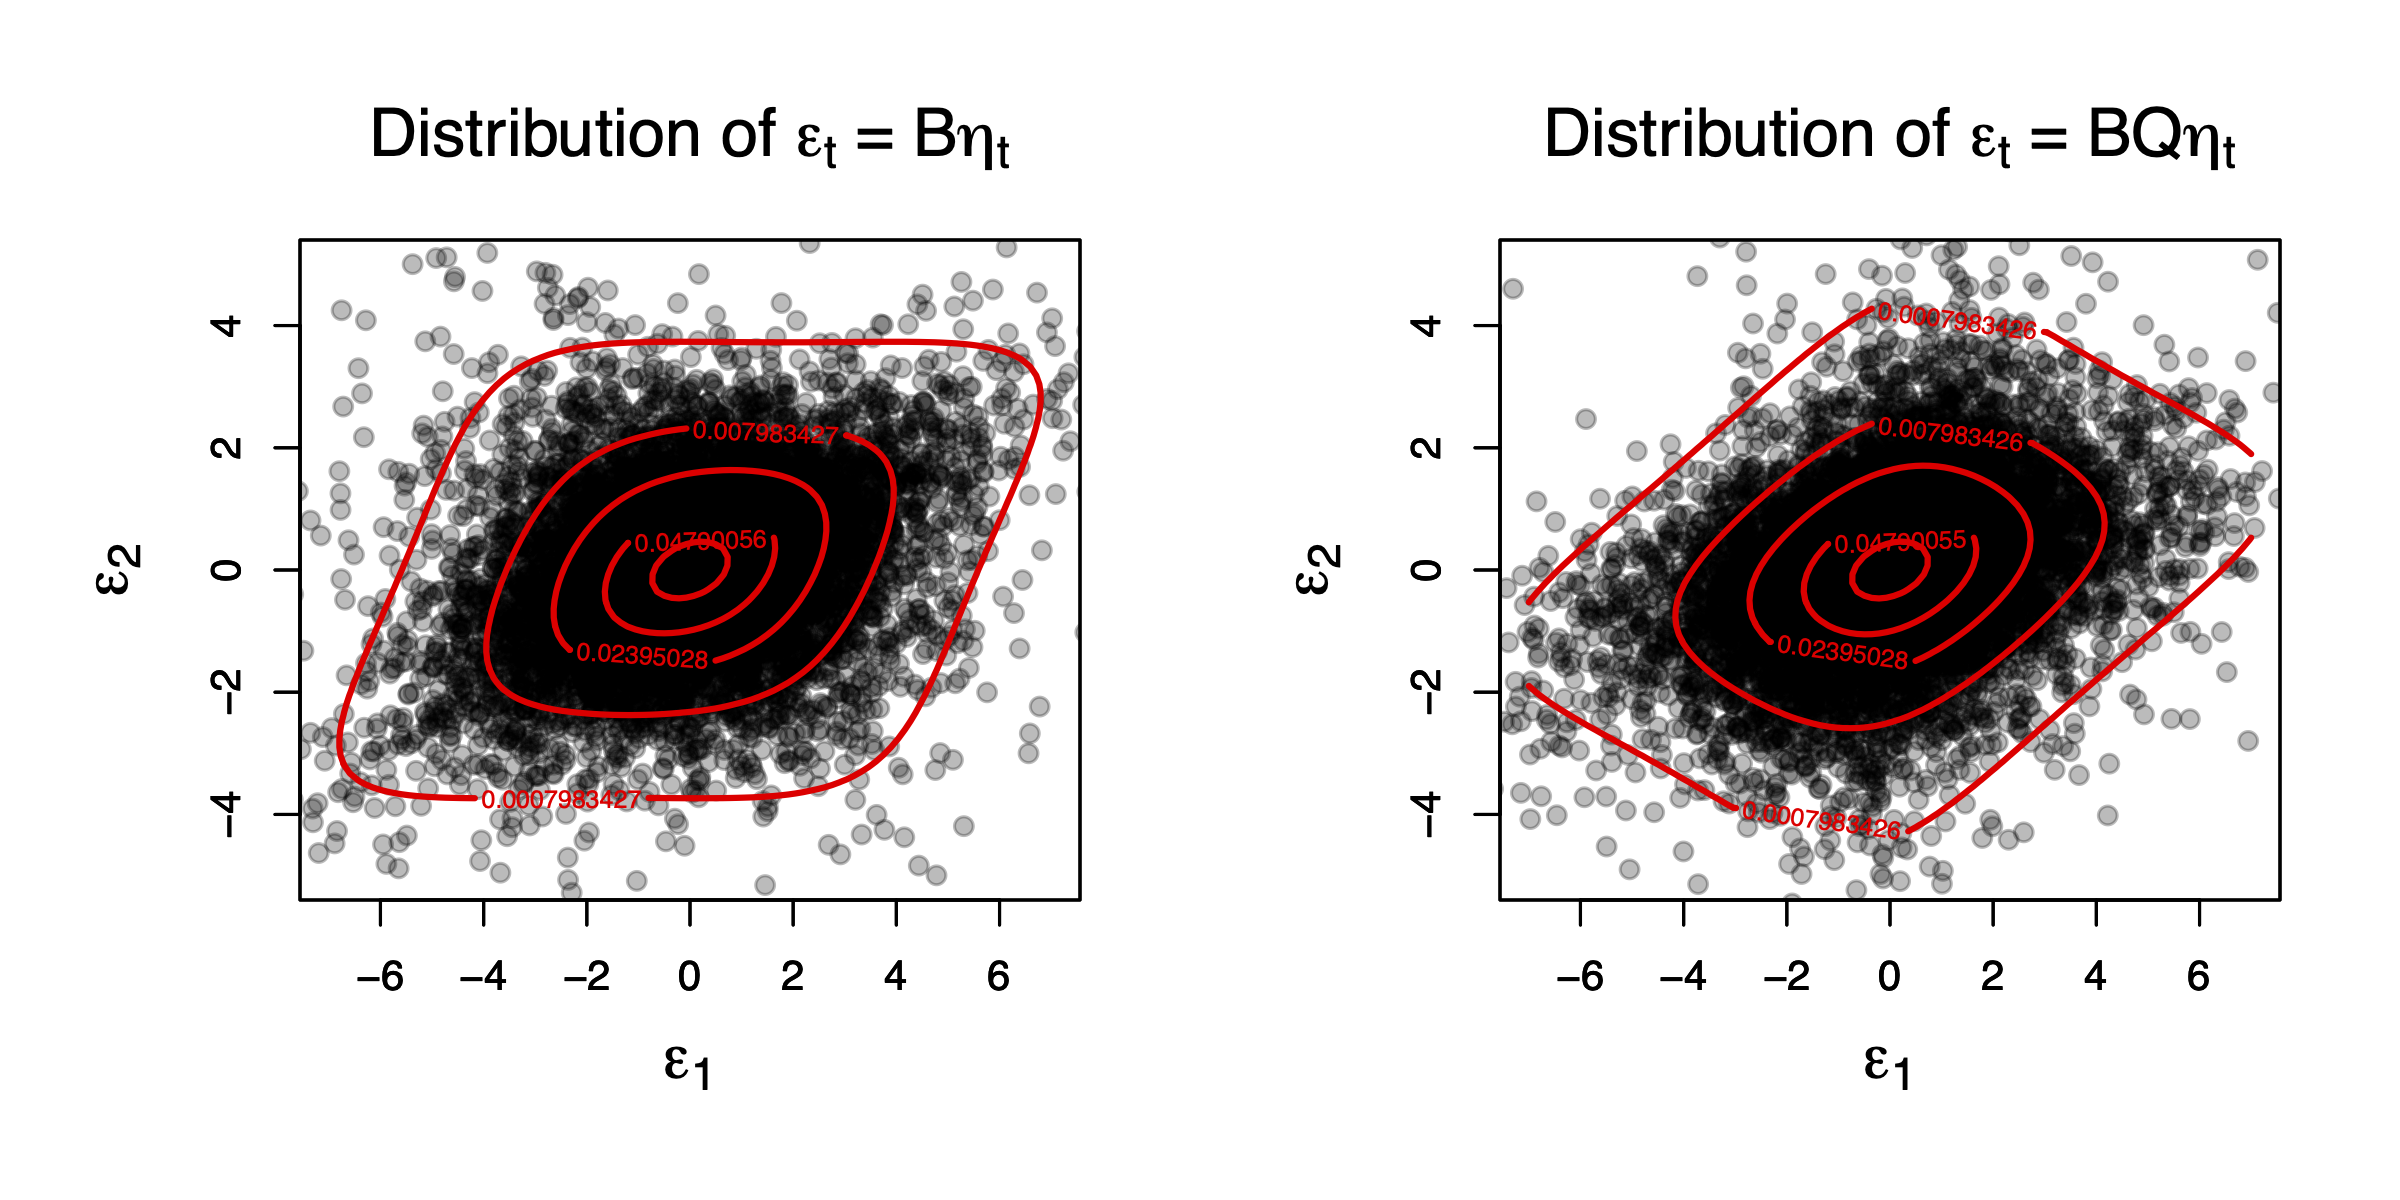
\includegraphics[width=0.95\linewidth]{images/Figure_D} \caption{XXXX.}\label{fig:preMadeFigureICAStudentStudent}
\end{figure}

\textbf{Relationship with Signal Processing Literature}

Task to be performed:

you observe \(n\) linear combinations of \(n\) \textbf{independent signals}; you want to estimate these linear combinations (\(\Leftrightarrow\) recover independent signals).

Without loss of generality, we can assume that \(BB' = Id\) (i.e.~\(B\) is orthogonal)

(If not the case, i.e.~if \(\mathbb{V}ar(\varepsilon_t)=\Omega \ne Id\), pre-multiply the data by \(\Omega^{-1/2}\)).

\textbf{Classical signal processing problem: Independent Component Analysis (ICA)}

Find \(B\) such that \(\varepsilon_t = B \eta_t\) (or \$\eta\_t= B' \varepsilon\_t \$) given that
i. you observe the \(\varepsilon_t\)'s,
ii. The components of \(\eta_t\) are independent,
iii. \(BB'=Id\) (\(B\) is orthogonal).

\begin{figure}
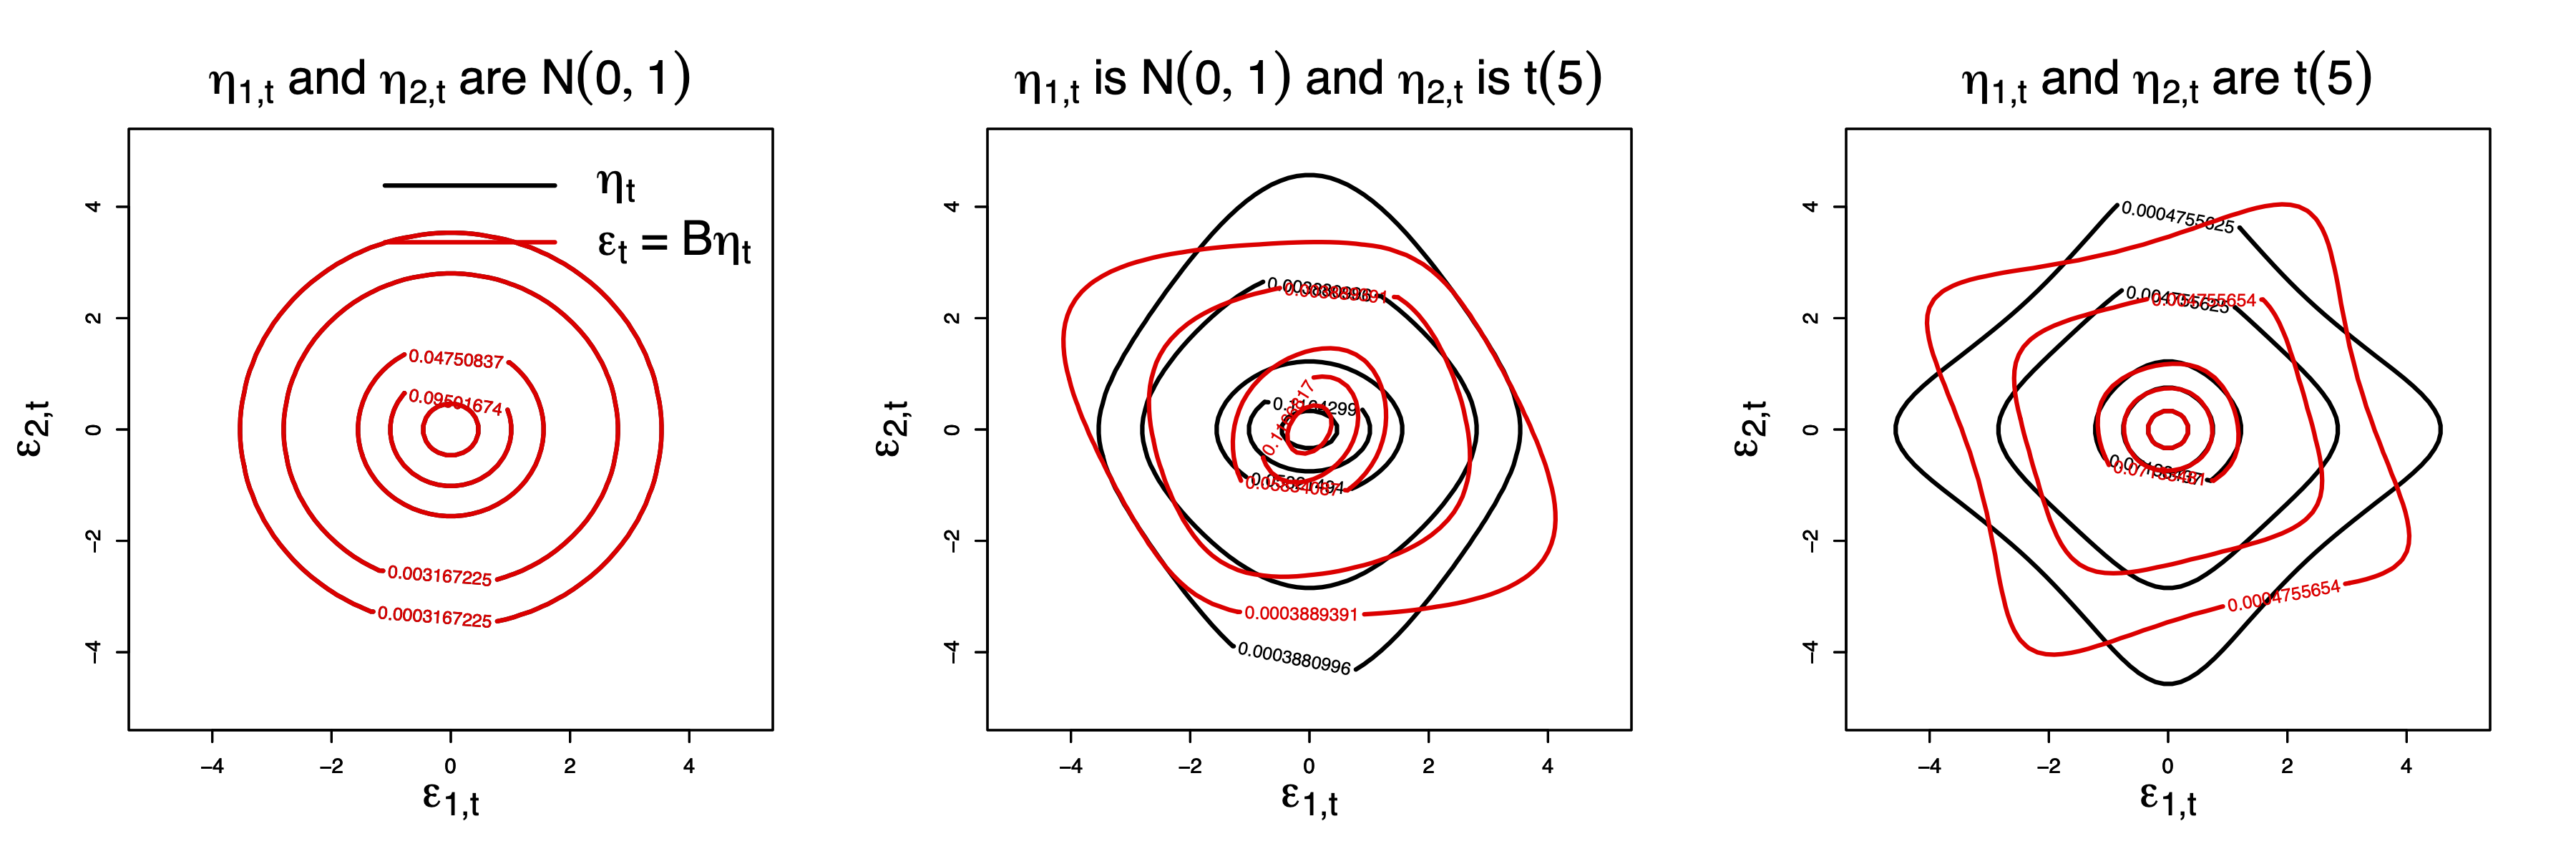
\includegraphics[width=0.95\linewidth]{images/Figure_E} \caption{XXXX.}\label{fig:ThreePlots}
\end{figure}

In all cases, we have \(\mathbb{V}ar(\varepsilon_t)=\mathbb{V}ar(\eta_t)=Id\). Assume you observe the distribution of \(\varepsilon_t\) (in \color{red}{red}). How to rotate \(\varepsilon_t\) to get obtain \emph{independent signals} (\(\eta_t = B'\varepsilon_t\))?

NB: \(\varepsilon_{1,t}\) and \(\varepsilon_{2,t}\) are not independent.

For instance: We have \(\mathbb{E}(\varepsilon_{2,t}|\varepsilon_{1,t}>4)<0\) (whereas \(\mathbb{E}(\eta_{2,t}|\eta_{1,t}>4)=0\)).

\begin{hypothesis}
\protect\hypertarget{hyp:NonGauss}{}\label{hyp:NonGauss}

We have:

\begin{enumerate}
\def\labelenumi{\roman{enumi}.}
\tightlist
\item
  The shocks \(\eta_t\) are i.i.d. with \(\mathbb{E}(\eta_t) = 0\) and \(\mathbb{V}ar(\eta_t) = Id.\)
\item
  The components \(\eta_{1,t}, \ldots, \eta_{n,t}\) are mutually independent.
  iii We have
  \[
  \boxed{Y_t = B_0 \eta_t,}
  \]
  with \(\mathbb{E}(Y_t) = Id\) (i.e.~\(B_0\) is orthogonal).
\end{enumerate}

\end{hypothesis}

\begin{theorem}[Eriksson, Koivunen (2004)]
\protect\hypertarget{thm:EK2004}{}\label{thm:EK2004}If Hypothesis \ref{hyp:NonGauss} is satisfied and if at most one of the components of \(\eta\) is Gaussian, then matrix \(B_0\) is identifiable up to the post multiplication by \(DP\), where \(P\) is a permutation matrix and \(D\) is a diagonal matrix whose diagonal entries are 1 or \(-1\).\}
\end{theorem}

\textbf{The PML approach}

We introduce a set of p.d.f. \(g_i (\eta_i), i=1,\ldots,n,\) and consider the \textbf{pseudo log-likelihood function}:
\begin{equation}
\log \mathcal{L}_T (B) = \sum^T_{t=1} \sum^n_{i=1} \log g_i (b'_i Y_t),\label{eq:pseudolog}
\end{equation}
where \(b_i\) is the \(i^{th}\) column of matrix \(B\) (or \(b'_i\) is the \(i^{th}\) row of \(B^{-1}\) since \(B^{-1}=B'\)).

The log-likelihood function \eqref{eq:pseudolog} is computed as if the errors \(\eta_{i,t}\) had the p.d.f. \(g_i (\eta_i)\).

A \textbf{pseudo maximum likelihood (PML) estimator} of matrix \(B\) maximizes the pseudo log-likelihood function:
\begin{equation}
\widehat{B_T} = \arg \max_B \sum^T_{t=1} \sum^n_{i=1} \log g_i (b'_i Y_t),\label{eq:optimprob}
\end{equation}

\centerline{$s.t. \;B'B = Id.$}

The restrictions \(B'B = Id\) can be eliminated by parameterizing \(B\).

\textbf{Cayley's representation:}

Any orthogonal matrix with no eigenvalue equal to \(-1\) can be written as
\begin{equation}
B(A) = (Id+A) (Id-A)^{-1},
\end{equation}
where \(A\) is a skew symmetric (or antisymmetric) matrix, such that \(A'=-A\).

There is a one-to-one relationship with \(A\), since:
\begin{equation}
A = (B(A)+Id)^{-1} (B(A)-Id).
\end{equation}

PML estimator of matrix \(B\): \(\widehat{B_T} = B(\hat{A}_T),\) where:
\begin{equation}
\hat{A}_T = \arg \max_{a_{i,j}, i>j} \sum^T_{t=1} \sum^n_{i=1} \log g_i [b_i (A)' Y_t].\label{eq:optimprob2}
\end{equation}

\textbf{Asymptotic properties of the PML approach}

\begin{hypothesis}
\protect\hypertarget{hyp:NonGauss2}{}\label{hyp:NonGauss2}

We have:

\begin{enumerate}
\def\labelenumi{\roman{enumi}.}
\tightlist
\item
  The functions \(\log g_i\), \(i=1,\ldots,n\), are twice continuously differentiable.
\item
  \(sup_{B: B'B = Id} \left|\sum^n_{i=1} \log g_i (b'_i y)\right| \leq h(y),\) where \(\mathbb{E}_0 [h (Y)] < \infty\).
\end{enumerate}

\end{hypothesis}

\begin{hypothesis}[Identification from the asymptotic FOC]
\protect\hypertarget{hyp:NonGauss3}{}\label{hyp:NonGauss3}The only solutions of the system of equations:
\[
\left\{
\begin{array}{l} \mathbb{E}_0 \left[b'_j Y_t \frac{d\log g_i}{d\eta} (b'_i Y_t)\right] = 0,\;  i \neq j, \\
B' B = Id,
\end{array}
\right.
\]
are the elements of \(\mathcal{P}_0 \equiv \mathcal{P}(B_0)\), which is the set of matrices obtained by permutation and sign change of the columns of \(B_0\).
\end{hypothesis}

\begin{hypothesis}[Local concavity]
\protect\hypertarget{hyp:NonGauss4}{}\label{hyp:NonGauss4}The asymptotic objective function is locally concave in a neighbourhood of a matrix \(B\) of \(\mathcal{P}(B_0)\), which is the case if and only if
\[
\mathbb{E}_0 \left[ \frac{d^2 \log g_i (\eta_{i,t})}{d\eta^2} + \frac{d^2 \log g_j (\eta_{j,t})}{d\eta^2} - \eta_{j,t} \frac{d\log g_j (\eta_{j,t})}{d\eta}- \eta_{i,t} \frac{d\log g_i (\eta_{i,t})}{d\eta} \right] < 0, \forall i<j,
\]
where \(\eta_{i,t}\) is the \(i^{th}\) component of the \(\eta_t\) associated with this particular element \(B\) of \(\mathcal{P}(B_0)\).
\end{hypothesis}

This condition is in particular satisfied under the following set of conditions: derived in Hyvarinen (1997) XXX
\begin{equation}
\mathbb{E}_0 \left[\frac{d^2 \log g_i(\eta_{i,t})}{d\eta^2} - \eta_{i,t} \frac{d\log g_i(\eta_{i,t})}{d\eta}\right] <0,\quad  i=1,\ldots, n. \label{eq:HKO}
\end{equation}

Hyperbolic secant and the subgaussian distributions (see table on next slide): either one, or the other satisfy the inequality \eqref{eq:HKO} {[}Hyvarinen, Karhunen, Oja, 2001 XXXX{]}.

XXXXXXXXXXXXXXX

Note: Except for the Gaussian distribution, we have \(E[d^2 \log g(X)/d \varepsilon^2 - X d\log g(X)/d \varepsilon] < 0\) (i.e.~Assumption,4 is satisfied) when these pseudo distributions coincide to the distribution of \(X\). The subGaussian distribution is a mixture of Gaussian distributions: \(X\) is drawn from this distribution if it is equal to \(BY - (1-B)Y\), where \(B\) is drawn from a Bernoulli distribution of parameter \(1/2\) and \(Y \sim \mathcal{N}(\sqrt{(\pi-2)/\pi},2/\pi)\).

Under Hypotheses \ref{NonGauss}-\ref{NonGauss4}, the PML estimator \(\widehat{B_T}\) of \(B_0\) is consistent (in \(\mathcal{P}_0\)) and asymptotically normal, with speed of convergence \(1/\sqrt{T}\).

The asymptotic variance-covariance matrix of \(vec \sqrt{T} (\widehat{B_T} - B_0)\) is \(A^{-1} \left[\begin{array}{cc} \Gamma & 0 \\ 0 & 0 \end{array} \right] (A')^{-1}\), where matrices \(A\) and \(\Gamma\) are detailed in Gouri'eroux, Monfort and Renne (2017) XXX.

The potential misspecification of pseudo-distributions \(g_i\) has no effect on the consistency of these specific PML estimators.

The previous proposition can be exploited to build a test whose null hypothesis is:

\emph{\(H_0\): \(B\) belongs to \(\mathcal{P}_0\), where \(\mathcal{P}_0\) is the set of orthogonal matrices obtained by permuting and changing the signs of the columns of a given orthogonal matrix \(B_0\).}

\textbf{Application: Structural VAR model}

Three dependent variables: inflation (\(\pi_t\)), economic activity (\(z_t\)) and the nominal short-term interest rate (\(r_t\)).

Structural shocks are posited monetary-policy, demand and supply shocks.

\(W_t\): set of information made of the past values of \(y_t= [\pi_t,z_t,r_t]\), that is \(\{y_{t-1},y_{t-2},\dots\}\), and of exogenous variables \(\{x_{t},x_{t-1},\dots\}\).

The reduced-form VAR model reads:
\[
y_t  = \underbrace{\mu + \sum_{i=1}^{p} \Phi_i y_{t-i} + \Theta x_t}_{a(W_t;\theta)} + u_t
\]
where the \(u_t\)'s are assumed to be serially independent, with zero mean and variance-covariance matrix \(\Sigma\).

U.S. data. 1959:IV to 2015:I at the quarterly frequency (\(T=224\)). Source: Federal Reserve Economic Database (FRED).

Two different measures of economic activity are considered: the output gap and the unemployment gap. Change in the log of oil prices added as an exogenous variable (\(x_t\)).

\(\mu\), \(\Phi_i\), \(\Theta\) and \(\Sigma\) are consistently estimated by OLS.

Jarque-Bera tests support the hypothesis of non-normality for all residuals.

We want to estimate the orthogonal matrix \(B\) such that \(u_t=SB \eta_t\), where

\begin{itemize}
\tightlist
\item
  \(S\) results from the Cholesky decomposition of \(\Sigma\) and
\item
  the components of \(\eta_t\) are independent, zero-mean with unit variance.
\end{itemize}

The PML approach is applied on standardized VAR residuals given by:
\[
\hat{S}_T^{-1}\underbrace{[y_t - a(W_t;\hat\theta_T)]}_{\mbox{VAR residuals}}.
\]
By construction of \(\hat{S}_T^{-1}\), it comes that the covariance matrix of these residuals is \(Id\).

Pseudo density functions: Distinct and asymmetric mixtures of Gaussian distributions.

Once \(B\) has been estimated, it remains to associate the structural shocks (monetary-policy, supply or demand) with the different components of \(\eta_{t}\).

\begin{itemize}
\tightlist
\item
  Contractionary \textbf{monetary-policy shocks}: negative impact on real activity and on inflation.
\item
  \textbf{Supply shock}: influences of opposite signs on economic activity and on inflation.
\item
  \textbf{Demand shock}: influences of same signs on economic activity and on inflation.
\end{itemize}

Important: This method does not rely on the assumption that specific impacts (e.g.~contemporaneous or long-run) are null.

Comparison of the previous IRFs with those stemming from ``recursive'' identification approaches based on specific short-run restrictions (SRRs).

SRRs approach (Section,\ref{Section:Standard}) are based on the assumptions that

\begin{enumerate}
\def\labelenumi{\alph{enumi}.}
\tightlist
\item
  \(Cov(\eta_t)=Id\),
\item
  the \(k^{th}\) structural shock does not contemporaneously affects the first \(k-1\) endogenous variables and
\item
  the contemporaneous effect of the \(k^{th}\) structural shock on the \(k^{th}\) dependent variable is positive.
\end{enumerate}

Under these assumptions, the structural shocks are given by \(S^{-1}u_t\).

SRR approaches assume --potentially wrongly-- that the contemporaneous impacts of some structural shocks on given variables are null.

The null hypothesis of these tests is \(H_0= (P \in \mathcal{P}(Id))\).
The null hypothesis \(H_0\) stating that the true value of \(B\) belongs to \(\mathcal{P}_0\) is not standard since it is a finite union of simple hypotheses \(H_{0,j} = (B = B_{j,0})\).

\textbf{First testing procedure:}

\begin{itemize}
\tightlist
\item
  Define the Wald statistics \(\hat\xi_{j,T}\), \(j \in J\):
  \begin{equation}
  \hat\xi_{j,T} = T [vec\hat{B}_T-vec B_{j,0}]'\hat{A}_T'
  \left[
  \begin{array}{cc}
  \hat{\Omega}^{-1}_T & 0\\
  0&0
  \end{array}
  \right]\hat{A}_T
  [vec\hat{B}_T-vec B_{j,0}],
  \end{equation}
  \(\hat{A}_T\) and \(\hat{\Omega}_T\) being consistent estimators of the matrices \(A\) and \(\Omega\).
\end{itemize}

Since the dimension of the asymptotic distribution of \(\sqrt{T}[vec\hat{B}_T-vec B_{j,0}]\) is \(\frac{1}{2}n(n-1)\), the asymptotic distribution of \(\hat\xi_{j,T}\) under \(H_{0,j}\) is \(\chi^2\left(\frac{1}{2}n(n-1)\right)\).

\begin{itemize}
\tightlist
\item
  Define \(\hat\xi_T = \underset{j \in J}{\min} \hat\xi_{j,T}\) as the test statistic for \(H_0\).
\item
  Under \(H_0\), \(\hat{B}_T\) converges to \(B_{j_0,0}\) (say).
\item
  By the asymptotic properties of the Wald statistics for simple hypotheses:
  \begin{equation}
  \hat\xi_{j_0,T} \overset{D}{\rightarrow} \chi^2\left(\frac{n(n-1)}{2}\right) \quad \mbox{and}\quad  \hat\xi_{j,T} \rightarrow \infty, \mbox{ if } j \ne j_0.
  \end{equation}
\end{itemize}

Under the null hypothesis, \(\hat\xi_T = \underset{j}{\min}\) \(\hat\xi_{j,T}\) is asymptotically equal to \(\hat\xi_{j_0,T}\) and its asymptotic distribution, \(\chi^2\left(\frac{1}{2}n(n-1)\right)\), does not depend on \(j_0\). Therefore \(\hat\xi_T\) is asymptotically a pivotal statistic for the null hypothesis \(H_0\) and the test of critical region \(\hat\xi_T \ge \chi^2_{1-\alpha}\left(\frac{1}{2}n(n-1)\right)\) is of asymptotic level \(\alpha\) and is consistent.

\textbf{Second testing procedure}

Define \(B_{0,T} = \underset{B \in \mathcal{P}_0}{\mbox{Argmin }} d(\hat{B}_T,B)\) where \(d\) is any distance, for instance the Euclidean one.

Under the null hypothesis \(H_0\): \((B \in \mathcal{P}_0)\), \(\hat{B}_T\) converges almost surely to an element of \(\mathcal{P}_0\) denoted by \(B_{j_0,0}\) and it is also the case for \(B_{0,T}\) since, asymptotically, we have \(B_{0,T}=B_{j_0,0}\).

Moreover:
\[
\sqrt{T}(\hat{B}_T - B_{0,T})=\sqrt{T}(\hat{B}_T - B_{j_0,0}) + \sqrt{T}(B_{j_0,0} - B_{0,T}),
\]
and, since \(B_{0,T}\) is almost surely asymptotically equal to \(B_{j_0,0}\), the asymptotic distribution of \(\sqrt{T}(\hat{B}_T - B_{0,T})\) under \(H_0\) is the same as that of \(\sqrt{T}(\hat{B}_T - B_{j_0,0})\).

This implies that
\[
\tilde\xi_{T} = T [vec\hat{B}_T-vec B_{0,T}]'\hat{A}_T'
\left[
\begin{array}{cc}
\hat{\Omega}^{-1}_T & 0\\
0&0
\end{array}
\right]\hat{A}_T
[vec\hat{B}_T-vec B_{0,T}]
\]
is asymptotically distributed as \(\chi^2\left(\frac{1}{2}n(n-1)\right)\) under \(H_0\).

An advantage of this second method is that it necessitates the computation of only one Wald test statistic.

We consider two specific SRR schemes:
* In both of them, it is assumed that the monetary-policy shock has no contemporaneous impact on \(\pi_t\) and \(y_t\).
* In SRR Scheme 1: Inflation is contemporaneously impacted by one structural shock only.
* In SRR Scheme 2: Economic activity is contemporaneously impacted by one structural shock only.
\textbackslash end\{itemize\}
* When economic activity is measured by means of the output gap, both SRRs are rejected at the 5\% level.

\textbf{Relation with the Heteroskedasticity Identification}

In some cases, where the \(\varepsilon_t\)'s are heteroskedastic, the \(B\) matrix can be identified

\href{/href\%7Bhttps://www.mitpressjournals.org/doi/10.1162/003465303772815727}{Rigobon (2003)},

\href{https://www.sciencedirect.com/science/article/pii/S0165188909001481\#!}{Lanne, Lutkepohl and Maciejowska (2010)}

Consider the case where we still have \(\varepsilon_t = B \eta_t\) but where \(\eta_t\)'s variance conditionally depends on a regime \(s_t \in \{1,\dots,M\}\). That is:
\[
\mathbb{V}ar(\eta_{k,t}|s_t) = \lambda_{s_t,k} \quad \mbox{for } k \in \{1,\dots,n\}
\]

Denoting by \(\Lambda_i\) the diagonal matrix whose diagonal entries are the \(\lambda_{i,k}\)'s, it comes that:
\[
\mathbb{V}ar(\eta_{t}|s_t) = \Lambda_{s_t},\quad \mbox{and}\quad \mathbb{V}ar(\varepsilon_{t}|s_t) = B\Lambda_{s_t}B'.
\]

Without loss of generality, it can be assumed that \(\Lambda_1=Id\).

In this context, \(B\) is identified, apart from sign reversal of its columns if for all \(k \ne j \in \{1,\dots,n\}\), there is a regime \(i\) s.t. \(\lambda_{i,k} \ne \lambda_{i,j}\). \href{https://www.sciencedirect.com/science/article/pii/S0165188909001481\#!}{Prop.1 in Lanne, L"utkepohl and Maciejowska (2010)}.

Bivariate regime case (\(M=2\)): \(B\) identified if the \(\lambda_{2,k}\)'s are all different. That is, identification is ensured if ``there is sufficient heterogeneity in the volatility changes'' {[}L"utkepohl and Netsunajev (2017)(\url{https://www.sciencedirect.com/science/article/pii/S2452306216300223}).

If the regimes \(s_t\) are exogenous and serially independent, then this situation is consistent with the ``non-Gaussian'' situation described in this section.

\hypertarget{factor-augmented-var-favar}{%
\subsection{Factor-Augmented VAR (FAVAR)}\label{factor-augmented-var-favar}}

VAR models are subject to the curse of dimensionality: If \(n\), is large, then the number of parameters (in \(n^2\)) explodes.

In the case where one suspects that the \(y_{i,t}\)'s are mainly driven by a small number of random sources, a factor structure may be imposed, and \textbf{principal component analysis} can be employed to estimate the relevant factors (\citet{Bernanke_Boivin_Eliasz_2005}).

Let us denote by \(F_t\) a \(k\)-dimensional vector of latent factors accounting for important shares of the variances of the \(y_{i,t}\)'s (with \(K \ll n\)) and by \(x_t\) is a small \(M\)-dimensional subset of \(y_t\) (with \(M \ll n\)). The following factor structure is posited:
\[
y_t = \Lambda^f F_t + \Lambda^x x_t + e_t,
\]
where the \(e_t\) are ``small'' serially and mutually i.i.d. error terms. That is \(F_t\) and \(x_t\) are supposed to drive most of the fluctuations of \(y_t\)'s components.

The model is complemented by positing a VAR dynamics for \([F_t',x_t']'\):
\begin{equation}
\left[\begin{array}{c}F_t\\x_t\end{array}\right] = \Phi(L)\left[\begin{array}{c}F_{t-1}\\ x_{t-1}\end{array}\right] + v_t.\label{eq:FAVAR}
\end{equation}

Standard identification techniques of structural shocks can be employed in Eq. \eqref{eq:FAVAR}: Cholesky approach can be used for instance if the last component of \(x_t\) is the short-term interest rate and if it is assumed that a MP shock has no contemporaneous impact on other macro-variables (in \(x_t\)).

In their identification procedure, \citet{Bernanke_Boivin_Eliasz_2005} exploit the fact that macro-finance variables can be decomposed in two sets ---fast-moving and slow-moving variables--- and that only the former reacts contemporaneously to monetary-policy shocks. Now, how to estimate the (unobserved) factors \(F_t\)? \citet{Bernanke_Boivin_Eliasz_2005} note that the first \(K+M\) PCA of the whole dataset (\(y_t\)), that they denote by \(\hat{C}(F_t,x_t)\) should span the same space as \(F_t\) and \(x_t)\). To get an estimate of \(F_t\), the dependence of \(\hat{C}(F_t,x_t)\) in \(x_t)\) has to be removed. This is done by regressing, by OLS, \(\hat{C}(F_t,x_t)\) on \(x_t)\) and on \(\hat{C}^*(F_t)\), where the latter is an estimate of the common components other than \(x_t\). To proxy for \(\hat{C}^*(F_t)\), \citet{Bernanke_Boivin_Eliasz_2005} take principal components from the set of slow-moving variables, that are not comtemporaneously correlated to \(x_t\). Vector \(\hat{F}_t\) is then computed as \(\hat{C}(F_t,x_t) - b_x x_t\), where \(b_x\) are the coefficients coming from the previous OLS regressions.

Note that this approach implies that the vectorial space spanned by \((\hat{F}_t,x_t)\) is the same as that spanned by \(\hat{C}(F_t,x_t)\).

Below, we employ this method on the dataset built by \citet{McCracken_Ng_2016} ---the \href{https://research.stlouisfed.org/wp/more/2015-012}{FRED:MD} database--- that includes 119 time series.

\begin{figure}
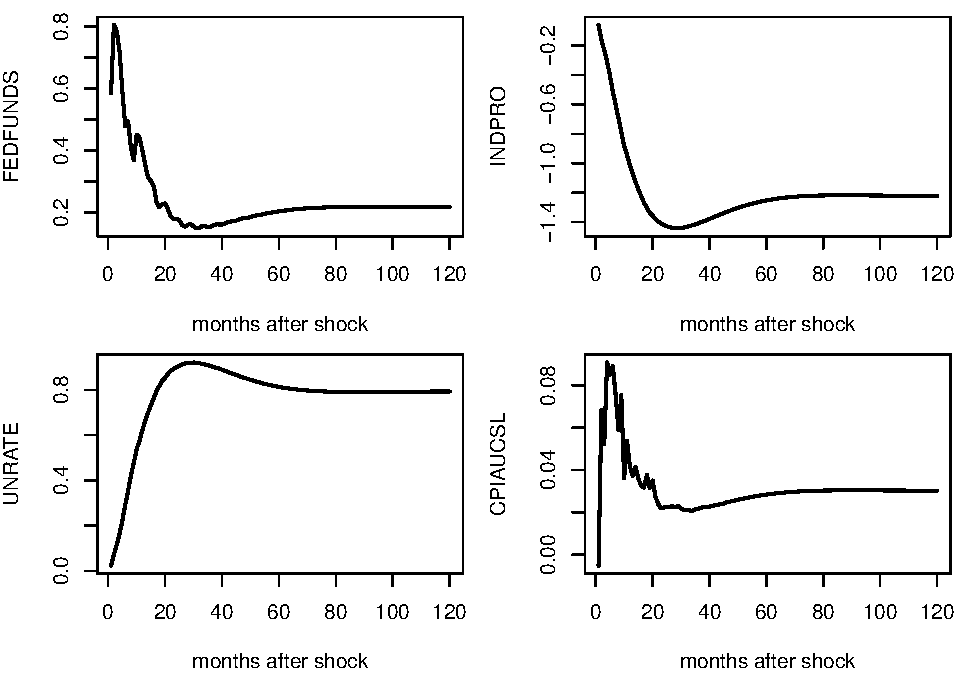
\includegraphics[width=0.95\linewidth]{AdvECTS_files/figure-latex/FAVAR-1} \caption{Responses of a monetary-policy shock. FAVAR approach of Bernanke, Boivin, and Eliasz (2005). FRED-MD dataset.}\label{fig:FAVAR}
\end{figure}

\hypertarget{Projections}{%
\subsection{Projections Methods}\label{Projections}}

Consider the infinite MA representation of \(y_t\) (Eq. \eqref{eq:InfMA}):
\[
y_t = \mu + \sum_{h=0}^\infty \color{blue}{\Psi_{h}} \eta_{t-h}.
\]
As seen in Section \ref{IRFSVARMA}, the entries \((i,j)\) of the sequence of the \(\Psi_h\) matrices define the IRF of \(\eta_{j,t}\) on \(y_{i,t}\).

Assume that you observe \(\eta_{j,t}\), then a consistent estimate of \(\Psi_{i,j,h}\) is simply obtained by the OLS regression of \(y_{i,t+h}\) on \(\eta_{j,t}\):
\begin{equation}
y_{i,t+h} = \mu_i + \Psi_{i,j,h}\eta_{j,t} + u_{i,j,t+h}.\label{eq:OLS1}
\end{equation}
Because the residuals \(u_{i,j,t+h}\) are autocorrelated (for \(h>0\)), estimates of the covariance of the OLS estimators of the \(\Psi_{i,j,h}\) then have to be based on robust estimators (e.g.~Newey-West, see Eq. \eqref{eq:NW}). This is the core idea of the \textbf{local projection approach} proposed by \citet{Jorda_2005}.

Now, how to proceed in the (usual) case where \(\eta_{j,t}\) is not observed? We consider two situations.

\textbf{Situation A: Without IV}

This corresponds to the original \citet{Jorda_2005}'s approach.

Assume that the structural shock of interest (\(\eta_{1,t}\), say) can be consistently obtained as the residual of a regression of a variable \(x_t\) on a set of control variables \(w_t\) independent from \(\eta_{1,t}\):
\begin{equation}
\eta_{1,t} = x_t - \mathbb{E}(x_t|w_t),\label{eq:xetaw}
\end{equation}
where \(\mathbb{E}(x_t|w_t)\) is affine in \(w_t\) and where \(w_t\) is an affine transformation of \(\eta_{2:n,t}\) and of past shocks \(\eta_{t-1},\eta_{t-2},\dots\).

Eq. \eqref{eq:xetaw} implies that, conditional on \(w_t\), the additional knowledge of \(x_t\) is useful only when it comes to forecast something that depends on \(\eta_{1,t}\). Hence, given that \(u_{i,1,t+h}\) (see Eq. \eqref{eq:OLS1}) is independent from \(\eta_{1,t}\) (it depends on \(\eta_{t+h},\dots,\eta_{t+1},{\color{blue}\eta_{2:n,t}},\eta_{t-1},\eta_{t-2},\dots\)), it comes that
\[
\mathbb{E}(u_{i,1,t+h}|x_t,w_t)= \mathbb{E}(u_{i,1,t+h}|w_t).
\]
This is the \emph{conditional mean independence} case.

Let's rewrite Eq. \eqref{eq:OLS1} as follows:
\begin{eqnarray*}
y_{i,t+h} &=& \mu_i + \Psi_{i,1,h}\eta_{1,t} + u_{i,1,t+h}\\
&=&  \mu_i + \Psi_{i,1,h}x_t  \color{blue}{-\Psi_{i,1,h}\mathbb{E}(x_t|w_t) + u_{i,1,t+h}},
\end{eqnarray*}

What precedes implies that the expectation of the blue term, conditional on \(x_t\) and \(w_t\), is linear in \(w_t\). Standard results in the conditional mean independence case imply that the regression of \(y_{i,t+h}\) on \(x_t\), controlling for \(w_t\), provides a consistent estimate of \(\Psi_{i,1,h}\):
\begin{equation}
y_{i,t+h} = \alpha_i + \Psi_{i,1,h}x_t + \beta'w_t + v_{i,t+h}.
\end{equation}

This is for instance consistent with the case where \([\Delta GDP_t, \pi_t,i_t]'\) follows a VAR(1) and the monetary-policy shock do not contemporaneously affect \(\Delta GDP_t\) and \(\pi_t\).

The IRFs can be estimated by LP, taking \(x_t = i_t\) and \(w_t = [\Delta GDP_t,\pi_t,\Delta GDP_{t-1}, \pi_{t-1},i_{t-1}]'\).

This approach closely relates to the SVAR Cholesky-based identification approach. Specifically, if \(w_t = [{\color{blue}y_{1,t},\dots,y_{k-1,t}}, y_{t-1}',\dots,y_{t-p}']'\), with \(k\le n\), and \(x_t = y_{k,t}\), then this approach corresponds, for \(h=0\), to the SVAR(\(p\)) Cholesky-based IRF (focusing on the responses to the \(k^{th}\) structural shock). However, the two approaches differ for \(h>0\), because the LP methodology does not assumes a VAR dynamics for \(y_t\).\footnote{This is reminiscent of the distinction betweem direct forecasting --based on regressions of \(y_{t+h}\) on \(\{y_t,y_{t-1},\dots\}\)-- and iterated forecasting --based on a recursive model where \(y_{t+1} = g(y_t,y_{t-1},\dots)+\varepsilon_{t+1}\), see \citet{Marcellino_et_al_2006}.}

\textbf{Situation B: IV approach}

Consider now that we have a valid instrument \(z_t\) for \(\eta_{1,t}\) (with \(\mathbb{E}(z_t)=0\)). That is:
\begin{equation}
\left\{
\begin{array}{llll}
(IV.i) & \mathbb{E}(z_t \eta_{1,t}) &\ne 0 & \mbox{(relevance condition)} \\
(IV.ii) & \mathbb{E}(z_t \eta_{j,t}) &= 0 \quad \mbox{for } j>1 & \mbox{(exogeneity condition)}
\end{array}\right.\label{eq:IV1}
\end{equation}
The instrument \(z_t\) can be used to identify the structural shock. Eq. \eqref{eq:IV1} implies that there exist \(\rho \ne 0\) and a mean-zero variable \(\xi_t\) such that:
\[
\eta_{1,t} = \rho z_t + \xi_t,
\]
where \(\xi_t\) is correlated neither to \(z_t\), nor to \(\eta_{j,t}\), \(j\ge2\).

\begin{proof}
Define \(\rho = \frac{\mathbb{E}(\eta_{1,t}z_t)}{\mathbb{V}ar(z_t)}\) and \(\xi_t = \eta_{1,t} - \rho z_t\). It is easily seen that \(\xi_t\) satisfies the moment restrictions given above.
\end{proof}

\citet{Ramey_2016_NBER} reviews the different approaches employed to construct monetary policy-shocks (the two main approaches are presented in \ref{exm:HighFreq} and \ref{RomerRomer} below). She has also collected time series of such shocks, see \href{https://econweb.ucsd.edu/~vramey/research.html\#mon}{her website}.

\begin{example}[Identification of Monetary-Policy Shocks Based on High-Frequency Data]
\protect\hypertarget{exm:HighFreq}{}\label{exm:HighFreq}

Instruments for monetary-policy shocks can be extracted from high-frequency market data associated with interest-rate products.

The quotes of all interest-rate-related financial products are sensitive to monetary-policy announcements. That is because these quotes mainly depends on investors' expectations regarding future short-term rates: \(\mathbb{E}_t(i_{t+s})\). Typically, if agents were risk-neutral, the maturity-\(h\) interest rate would approximatively be given by:
\[
i_{t,h} \approx \mathbb{E}_t\left(\frac{1}{h}\int_{0}^{h} i_{t+s} ds\right) = \frac{1}{h}\int_{0}^{h} \mathbb{E}_t\left(i_{t+s}\right) ds.
\]
In general, changes in \(\mathbb{E}_t(i_{t+s})\), for \(s>0\), can be affected by all types of shocks that may trigger a reaction by the central bank.

However, if a MP announcement takes place between \(t\) and \(t+\epsilon\), then most of \(\mathbb{E}_{t+\epsilon}(i_{t+s})-\mathbb{E}_t(i_{t+s})\) is to be attributed to the MP shock (see Figure \ref{fig:HighFreq}, from \citet{Gurkaynak_et_al_2005}). Hence, a monthly time series of MP shocks can be obtained by summing, over each month, the changes \(i_{t+ \epsilon,h} - i_{t,h}\) associated with a given interest rate (T-bills, futures, swaps) and a given maturity \(h\).

See among others: \citet{KUTTNER2001523}, \citet{Cochrane_Piazzesi_2002},\citet{Gurkaynak_et_al_2005}, \citet{Piazzesi_Swanson_2008}, \citet{Gertler_Karadi_2015}.

\begin{figure}
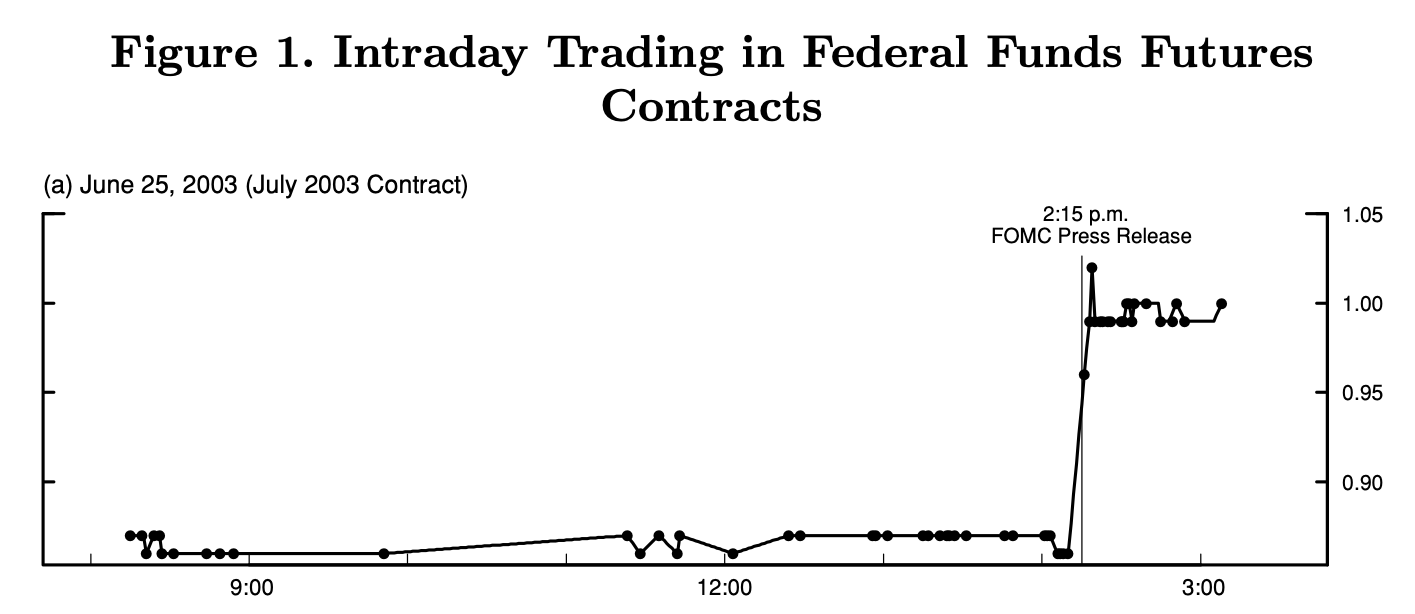
\includegraphics[width=0.95\linewidth]{images/GSS2005_HFI} \caption{Source: Gurkaynak, Sack and Swanson (2005). Transaction rates of Federal funds futures on June 25, 2003, day on which a regularly scheduled FOMC meeting was scheduled. At 2:15 p.m., the FOMC announced that it was lowering its target for the federal funds rate from 1.25\% to 1\%, while many market participants were expecting a 50 bp cut. This shows that (i) financial markets seem to fully adjust to the policy action within just a few minutes and (ii) the federal funds rate surprise is not necessarily in the same direction as the federal funds rate action itself.}\label{fig:HighFreq}
\end{figure}

\end{example}

\begin{example}[Identification of Monetary-Policy Shocks Based on the Narrative Approach]
\protect\hypertarget{exm:RomerRomer}{}\label{exm:RomerRomer}\citet{Romer_Romer_2004} propose a two-step approach:

\begin{enumerate}
\def\labelenumi{\alph{enumi}.}
\tightlist
\item
  derive a series for Federal Reserve intentions for the federal funds rate (the explicit target of the Fed) around FOMC meetings,
\item
  control for Federal Reserve forecasts.
\end{enumerate}

This gives a measure of intended monetary policy actions not driven by information about future economic developments.
a. ``intentions'' are measured as a combination of narrative and quantitative evidence. Sources: (among others) Minutes of FOMC and ``Blue Books''.
b. Controls = variables spanning the information the Federal Reserve has about future developments. Data: Federal Reserve's internal forecasts (inflation, real output and unemployment), ``Greenbook's forecasts'' -- usually issued 6 days before the FOMC meeting.

The shock measure is the residual series in the linear regression of (a) on (b).
\end{example}

There are two main IV approaches to estimate IRFs see \citet{Stock_Watson_2018}:

\begin{enumerate}
\def\labelenumi{\alph{enumi}.}
\tightlist
\item
  The LP-IV approach, where \(y_t\)'s DGP is left unspecified,
\item
  The SVAR-IV approach.
\end{enumerate}

The LP-IV approach is based on a set of IV regressions (for each variable of interest, one for each forecast horizon). The SVAR-IV approach is based on IV regressions of VAR innovations only (one for each series of VAR innovations).

If the VAR adequately captures the DGP, then the IV-SVAR is optimal for all horizons. However, if the VAR is misspecified, then specification errors are compounded at each horizon and a local projection method would lead to better results.

\textbf{Situation B.1: SVAR-IV approach}

Assume you have consistent estimates of \(\varepsilon_t = B\eta_t\), these estimates (\(\hat\varepsilon_{t}\)) coming from the estimation of a VAR model. You have, for \(i \in \{1,\dots,n\}\):
\begin{eqnarray}
\varepsilon_{i,t} &=& b_{i,1} \eta_{1,t} + u_{i,t} (\#eq:eps_rho)\\
&=& b_{i,1} \rho z_t + \underbrace{b_{i,1}\xi_t + u_{i,t}}_{\perp z_t}. \nonumber
\end{eqnarray}
(\(u_{i,t}\) is a linear combination of the \(\eta_{j,t}\)'s, \(j\ge2\)).

Hence, up to a multiplicative factor (\(\rho\)), the (OLS) regressions of the \(\hat\varepsilon_{i,t}\)'s on \(z_t\) provide consistent estimates of the \(b_{i,1}\)'s.

Combined with the estimated VAR (the \(\Phi_k\) matrices), this provides consistent estimates of the IRFs of \(\eta_{1,t}\) on \(y_t\), though up to a multiplicative factor. This scale ambiguity can be solved by rescaling the structural shock (``unit-effect normalisation'', see \citet{Stock_Watson_2018}). Let us consider \(\tilde\eta_{1,t}=b_{1,1}\eta_{1,t}\); by construction, \(\tilde\eta_{1,t}\) has a one-unit contemporaneous effect on \(y_{1,t}\). Denoting by \(\tilde{B}_{i,1}\) the contemporaneous impact of \(\tilde\eta_{1,t}\), we get:
\[
\tilde{B}_{1} = \frac{1}{b_{1,1}} {B}_{1},
\]
where \(B_{1}\) denotes the \(1^{st}\) column of \(B\) and \(\tilde{B}_{1}=[1,\tilde{B}_{2,1},\dots,\tilde{B}_{n,1}]'\).

Eq. @ref(eq:eps\_rho) gives:
\begin{eqnarray*}
\varepsilon_{1,t} &=& \tilde\eta_{1,t} + u_{1,t}\\
\varepsilon_{i,t} &=& \tilde{B}_{i,1} \tilde\eta_{1,t} + u_{i,t}.
\end{eqnarray*}
This suggests that \(\tilde{B}_{i,1}\) can be estimated by regressing \(\varepsilon_{i,t}\) on \(\varepsilon_{1,t}\), using \(z_t\) as an instrument.

What about inference? Once cannot use the usual TSLS standard deviations because the \(\varepsilon_{i,t}\)'s are not directly observed. Bootstrap procedures can be resorted to. \citet{Stock_Watson_2018} propose, in particular, a Gaussian parametric bootstrap:

Assume you have estimated \(\{\widehat{\Phi}_1,\dots,\widehat{\Phi}_p,\widehat{B}_1\}\) using the SVAR-IV approach based on a size-\(T\) sample. Generate \(N\) (where \(N\) is large) size-\(T\) samples from the following VAR:
\[
\left[
\begin{array}{cc}
\widehat{\Phi}(L) & 0 \\
0 & \widehat{\rho}(L)
\end{array}
\right]
\left[
\begin{array}{c}
y_t \\
z_t
\end{array}
\right] =
\left[
\begin{array}{c}
\varepsilon_t \\
e_t
\end{array}
\right],
\]
\[
\mbox{where} \quad \left[
\begin{array}{c}
\varepsilon_t \\
e_t
\end{array}
\right]\sim \, i.i.d.\,\mathcal{N}\left(\left[\begin{array}{c}0\\0\end{array}\right],
\left[\begin{array}{cc}
\Omega & S'_{\varepsilon,e}\\
S_{\varepsilon,e}& \sigma^2_{e}
\end{array}\right]
\right),
\]
where \(\widehat{\rho}(L)\) and \(\sigma^2_{e}\) result from the estimation of an AR process for \(z_t\), and where \(\Omega\) and \(S_{\varepsilon,e}\) are sample covariances for the VAR/AR residuals.

For each simulated sample (of \(\tilde{y}_t\) and \(\tilde{z}_t\), say), estimate \(\{\widetilde{\widehat{\Phi}}_1,\dots,\widetilde{\widehat{\Phi}}_p,\widetilde{\widehat{B}}_1\}\) and associated \(\widetilde{\Psi}_{i,1,h}\). This provides e.g.~a sequence of \(N\) estimates of \(\Psi_{i,1,h}\), from which quantiles and conf. intervals can be deduced.

\begin{Shaded}
\begin{Highlighting}[]
\CommentTok{\# Load vars package:}
\FunctionTok{library}\NormalTok{(vars)}
\FunctionTok{library}\NormalTok{(AEC)}
\FunctionTok{data}\NormalTok{(}\StringTok{"USmonthly"}\NormalTok{)}
\NormalTok{First.date }\OtherTok{\textless{}{-}} \StringTok{"1990{-}05{-}01"}
\NormalTok{Last.date }\OtherTok{\textless{}{-}} \StringTok{"2012{-}6{-}01"}
\NormalTok{indic.first }\OtherTok{\textless{}{-}} \FunctionTok{which}\NormalTok{(USmonthly}\SpecialCharTok{$}\NormalTok{DATES}\SpecialCharTok{==}\NormalTok{First.date)}
\NormalTok{indic.last  }\OtherTok{\textless{}{-}} \FunctionTok{which}\NormalTok{(USmonthly}\SpecialCharTok{$}\NormalTok{DATES}\SpecialCharTok{==}\NormalTok{Last.date)}
\NormalTok{USmonthly   }\OtherTok{\textless{}{-}}\NormalTok{ USmonthly[indic.first}\SpecialCharTok{:}\NormalTok{indic.last,]}
\NormalTok{shock.name }\OtherTok{\textless{}{-}} \StringTok{"FF4\_TC"} \CommentTok{\#"FF4\_TC", "ED2\_TC", "ff1\_vr", "rrshock83b"}
\NormalTok{indic.shock.name }\OtherTok{\textless{}{-}} \FunctionTok{which}\NormalTok{(}\FunctionTok{names}\NormalTok{(USmonthly)}\SpecialCharTok{==}\NormalTok{shock.name)}
\NormalTok{Z }\OtherTok{\textless{}{-}} \FunctionTok{matrix}\NormalTok{(USmonthly[,indic.shock.name],}\AttributeTok{ncol=}\DecValTok{1}\NormalTok{)}
\FunctionTok{plot}\NormalTok{(USmonthly}\SpecialCharTok{$}\NormalTok{DATES,Z,}\AttributeTok{type=}\StringTok{"l"}\NormalTok{,}\AttributeTok{xlab=}\StringTok{""}\NormalTok{,}\AttributeTok{ylab=}\StringTok{""}\NormalTok{)}
\end{Highlighting}
\end{Shaded}

\begin{figure}
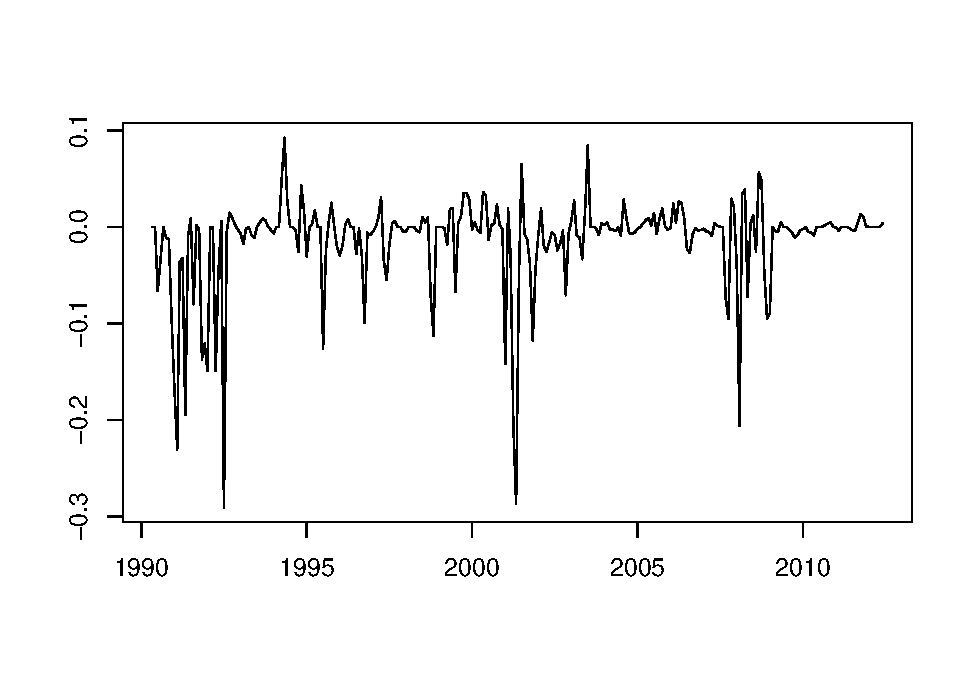
\includegraphics[width=0.95\linewidth]{AdvECTS_files/figure-latex/essaiIV0-1} \caption{Gertler-Karadi monthly shocks, fed funds futures 3 months.}\label{fig:essaiIV0}
\end{figure}

\begin{Shaded}
\begin{Highlighting}[]
\NormalTok{considered.variables }\OtherTok{\textless{}{-}} \FunctionTok{c}\NormalTok{(}\StringTok{"GS1"}\NormalTok{,}\StringTok{"LIP"}\NormalTok{,}\StringTok{"LCPI"}\NormalTok{,}\StringTok{"EBP"}\NormalTok{)}
\NormalTok{y }\OtherTok{\textless{}{-}} \FunctionTok{as.matrix}\NormalTok{(USmonthly[,considered.variables])}
\NormalTok{n }\OtherTok{\textless{}{-}} \FunctionTok{length}\NormalTok{(considered.variables)}
\FunctionTok{colnames}\NormalTok{(y) }\OtherTok{\textless{}{-}}\NormalTok{ considered.variables}
\NormalTok{res.svar.iv }\OtherTok{\textless{}{-}} \FunctionTok{svar.iv}\NormalTok{(y,Z,}\AttributeTok{p =} \DecValTok{4}\NormalTok{,}
                       \AttributeTok{names.of.variables=}\NormalTok{considered.variables,}
                       \AttributeTok{nb.periods.IRF =} \DecValTok{20}\NormalTok{,}
                       \AttributeTok{z.AR.order=}\DecValTok{1}\NormalTok{, }\CommentTok{\# This is used in the parametric bootstrap only}
                       \AttributeTok{nb.bootstrap.replications =} \DecValTok{100}\NormalTok{, }\CommentTok{\# This is used in the parametric bootstrap only}
                       \AttributeTok{confidence.interval =} \FloatTok{0.90}\NormalTok{, }\CommentTok{\# This is used in the parametric bootstrap only}
                       \AttributeTok{indic.plot=}\DecValTok{1}\NormalTok{)}
\end{Highlighting}
\end{Shaded}

\begin{figure}
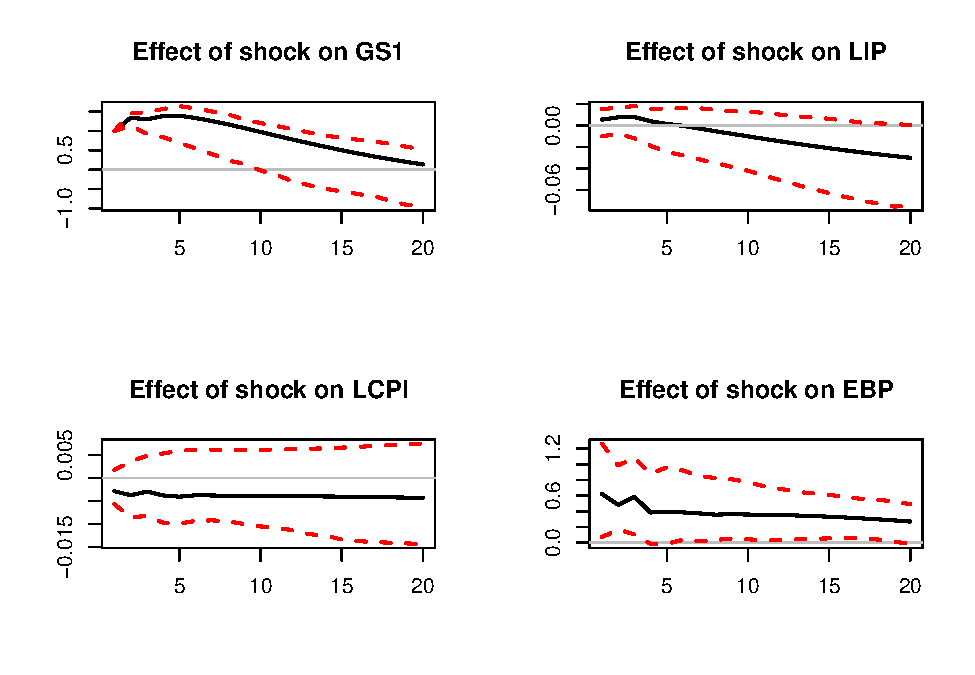
\includegraphics[width=0.95\linewidth]{AdvECTS_files/figure-latex/essaiIV1-1} \caption{Reponses to a monetary-policy shock, SVAR-IV approach.}\label{fig:essaiIV1}
\end{figure}

\textbf{Situation B.2: LP-IV}

If you do not want to posit a VAR-type dynamics for \(y_t\) --e.g.~because you suspect that the true generating model may be a non-invertible VARMA model-- you can directly proceed by IV-projection methods to obtain the \(\tilde\Psi_{i,1,h}\equiv \Psi_{i,1,h}/b_{1,1}\) (that are the IRFs of \(\tilde\eta_{1,t}\) on \(y_{i,t}\)).

However, Assumptions (IV.i) and (IV.ii) (Eq. \eqref{eq:IV1}) have to be complemented with (IV.iii):
\begin{equation*}
\begin{array}{llll}
(IV.iii) & \mathbb{E}(z_t \eta_{j,t+h}) &= 0 \, \mbox{ for } h \ne 0 & \mbox{(lead-lag exogeneity)}
\end{array}
\end{equation*}

When (IV.i), (IV.ii) and (IV.iii) are satisfied, \(\tilde\Psi_{i,1,h}\) can be estimated by regressing \(y_{i,t+h}\) on \(y_{1,t}\), using \(z_t\) as an instrument, i.e.~by considering the TSLS estimation of:
\begin{equation}
y_{i,t+h} = \alpha_i + \tilde\Psi_{i,1,h}y_{1,t} + \nu_{i,t+h},\label{eq:regIV1}
\end{equation}
where \(\nu_{i,t+h}\) is correlated to \(y_{1,t}\), but not to \(z_t\).

We have indeed:
\begin{eqnarray*}
y_{1,t} &=& \alpha_1 + \tilde\eta_{1,t} + v_{1,t}\\
y_{i,t+h} &=& \alpha_i + \tilde\Psi_{i,1,h}\tilde\eta_{1,t} + v_{i,t+h},
\end{eqnarray*}
where the \(v_{i,t+h}\)'s are uncorrelated to \(z_t\) under (IV.i), (IV.ii) and (IV.iii).

Note again that, for \(h>0\), the \(v_{i,t+h}\) (and \(\nu_{i,t+h}\)) are auto-correlated. Newey-West corrections therefore have to be used to compute std errors of the \(\tilde\Psi_{i,1,h}\)'s estimates.

Consider the linear regression:
\[
\mathbf{Y} = \mathbf{X}\boldsymbol\beta + \boldsymbol\varepsilon,
\]
where \(\mathbb{E}(\boldsymbol\varepsilon)=0\), but where the explicative variables \(\mathbf{X}\) are supposed to be correlated to the residuals \(\boldsymbol\varepsilon\).

Moreover, the \(\boldsymbol\varepsilon\) are supposed to be possibly heteroskedastic and auto-correlated.

We consider the instruments \(\mathbf{Z}\), with \(\mathbb{E}(\mathbf{X}'\mathbf{Z}) \ne 0\) but \(\mathbb{E}(\boldsymbol\varepsilon'\mathbf{Z}) = 0\).

The IV estimator of \(\boldsymbol\beta\) is obtained by regressing \(\hat{\mathbf{Y}}\) on \(\hat{\mathbf{X}}\), where \(\hat{\mathbf{Y}}\) and \(\hat{\mathbf{X}}\) are the respective residuals of the regressions of \(\mathbf{Y}\) and \(\mathbf{X}\) on \(\mathbf{Z}\).
\begin{eqnarray*}
\mathbf{b}_{iv} &=& [\mathbf{X}'\mathbf{Z}(\mathbf{Z}'\mathbf{Z})^{-1}\mathbf{Z}'\mathbf{X}]^{-1}\mathbf{X}'\mathbf{Z}(\mathbf{Z}'\mathbf{Z})^{-1}\mathbf{Z}'\mathbf{Y}\\
\mathbf{b}_{iv} &=& \boldsymbol\beta + \frac{1}{\sqrt{T}}\underbrace{T[\mathbf{X}'\mathbf{Z}(\mathbf{Z}'\mathbf{Z})^{-1}\mathbf{Z}'\mathbf{X}]^{-1}\mathbf{X}'\mathbf{Z}(\mathbf{Z}'\mathbf{Z})^{-1}}_{=Q(\mathbf{X},\mathbf{Z}) \overset{p}{\rightarrow} \mathbf{Q}_{xz}}\underbrace{\sqrt{T}\left(\frac{1}{T}\mathbf{Z}'\boldsymbol\varepsilon\right)}_{\overset{d}{\rightarrow} \mathcal{N}(0,S)},
\end{eqnarray*}
where \(\mathbf{S}\) is the long-run variance of \(\mathbf{z}_t\varepsilon_t\) (see next slide).

The asymptotic covariance matrix of \(\sqrt{T}\mathbf{b}_{iv}\) is \(\mathbf{Q}_{xz} \mathbf{S} \mathbf{Q}_{xz}'\).

The covariance matrix of \(\mathbf{b}_{iv}\) can be approximated by \(\frac{1}{T}Q(\mathbf{X},\mathbf{Z})\hat{\mathbf{S}}Q(\mathbf{X},\mathbf{Z})'\) where \(\hat{\mathbf{S}}\) is the Newey-West estimator of \(\mathbf{S}\) (see Eq. \eqref{eq:NW})

(IV.iii) is usually not restrictive for \(h>0\) (\(z_t\) is usually not affected by future shocks). By contrast, it may be restrictive for \(h<0\). This can be solved by adding controls in Regression \eqref{eq:regIV1}. These controls should span the space of \(\{\eta_{t-1},\eta_{t-2},\dots\}\).

If \(z_t\) is suspected to be correlated to past values of \(\eta_{1,t}\) but not to the \(\eta_{j,t}\)'s, \(j>1\), then one can add lags of \(z_t\) as controls (method e.g.~advocated by Ramey, 2016, p.108, considering the instrument by \citet{Gertler_Karadi_2015}).

In the general case, one can use lags of \(y_t\) as controls. Note that, even if (IV.iii) holds, adding controls may reduce the variance of the regression error.

As noted by \citet{Stock_Watson_2018}, the relevant variance is the long-run variance of the instrument-times-error term. They also recommend (p.926) using leads and lags of \(z_t\) to improve efficiency.

\begin{Shaded}
\begin{Highlighting}[]
\NormalTok{res.LP.IV }\OtherTok{\textless{}{-}} \FunctionTok{make.LPIV.irf}\NormalTok{(y,Z,}
                           \AttributeTok{nb.periods.IRF =} \DecValTok{20}\NormalTok{,}
                           \AttributeTok{nb.lags.Y.4.control=}\DecValTok{4}\NormalTok{,}
                           \AttributeTok{nb.lags.Z.4.control=}\DecValTok{4}\NormalTok{,}
                           \AttributeTok{indic.plot =} \DecValTok{1}\NormalTok{, }\CommentTok{\# Plots are displayed if = 1.}
                           \AttributeTok{confidence.interval =} \FloatTok{0.90}\NormalTok{)}
\end{Highlighting}
\end{Shaded}

\begin{verbatim}
## [1] "LP-IV approach, Currently working on horizon h=0"
## [1] "LP-IV approach, Currently working on horizon h=1"
## [1] "LP-IV approach, Currently working on horizon h=2"
## [1] "LP-IV approach, Currently working on horizon h=3"
## [1] "LP-IV approach, Currently working on horizon h=4"
## [1] "LP-IV approach, Currently working on horizon h=5"
## [1] "LP-IV approach, Currently working on horizon h=6"
## [1] "LP-IV approach, Currently working on horizon h=7"
## [1] "LP-IV approach, Currently working on horizon h=8"
## [1] "LP-IV approach, Currently working on horizon h=9"
## [1] "LP-IV approach, Currently working on horizon h=10"
## [1] "LP-IV approach, Currently working on horizon h=11"
## [1] "LP-IV approach, Currently working on horizon h=12"
## [1] "LP-IV approach, Currently working on horizon h=13"
## [1] "LP-IV approach, Currently working on horizon h=14"
## [1] "LP-IV approach, Currently working on horizon h=15"
## [1] "LP-IV approach, Currently working on horizon h=16"
## [1] "LP-IV approach, Currently working on horizon h=17"
## [1] "LP-IV approach, Currently working on horizon h=18"
## [1] "LP-IV approach, Currently working on horizon h=19"
## [1] "LP-IV approach, Currently working on horizon h=20"
\end{verbatim}

\begin{figure}
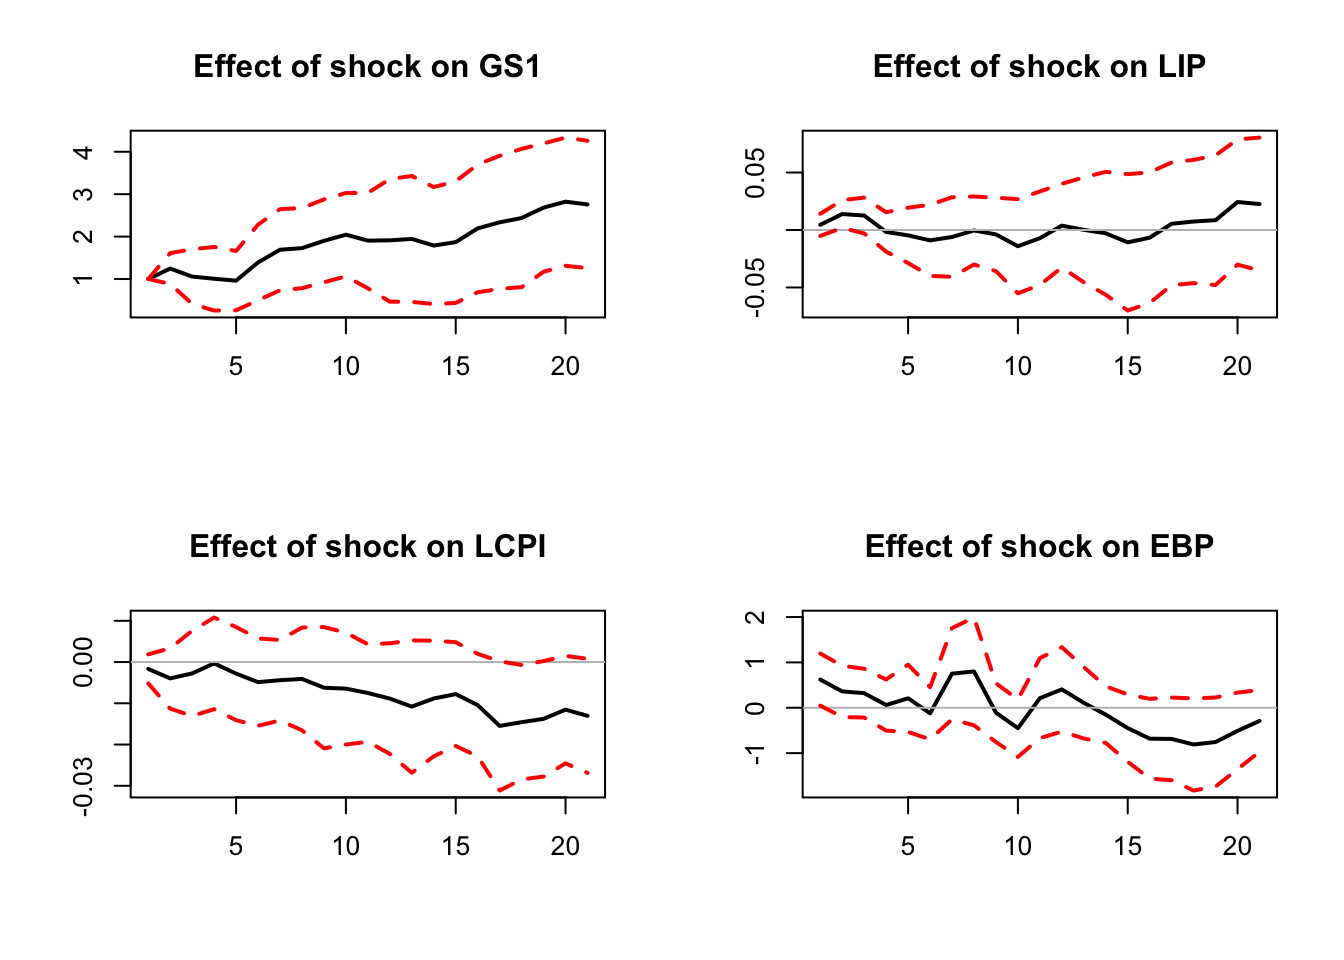
\includegraphics[width=0.95\linewidth]{AdvECTS_files/figure-latex/essaiIV-1} \caption{Reponses to a monetary-policy shock, LP-IV approach.}\label{fig:essaiIV}
\end{figure}

\hypertarget{append}{%
\chapter{Appendix}\label{append}}

\hypertarget{statistical-tables}{%
\section{Statistical Tables}\label{statistical-tables}}

\begin{table}

\caption{\label{tab:Normal}Quantiles of the $\mathcal{N}(0,1)$ distribution. If $a$ and $b$ are respectively the row and column number; then the corresponding cell gives $\mathbb{P}(0<X\le a+b)$, where $X \sim \mathcal{N}(0,1)$.}
\centering
\begin{tabular}[t]{l|r|r|r|r|r|r|r|r|r|r}
\hline
  & 0 & 0.01 & 0.02 & 0.03 & 0.04 & 0.05 & 0.06 & 0.07 & 0.08 & 0.09\\
\hline
0 & 0.5000 & 0.6179 & 0.7257 & 0.8159 & 0.8849 & 0.9332 & 0.9641 & 0.9821 & 0.9918 & 0.9965\\
\hline
0.1 & 0.5040 & 0.6217 & 0.7291 & 0.8186 & 0.8869 & 0.9345 & 0.9649 & 0.9826 & 0.9920 & 0.9966\\
\hline
0.2 & 0.5080 & 0.6255 & 0.7324 & 0.8212 & 0.8888 & 0.9357 & 0.9656 & 0.9830 & 0.9922 & 0.9967\\
\hline
0.3 & 0.5120 & 0.6293 & 0.7357 & 0.8238 & 0.8907 & 0.9370 & 0.9664 & 0.9834 & 0.9925 & 0.9968\\
\hline
0.4 & 0.5160 & 0.6331 & 0.7389 & 0.8264 & 0.8925 & 0.9382 & 0.9671 & 0.9838 & 0.9927 & 0.9969\\
\hline
0.5 & 0.5199 & 0.6368 & 0.7422 & 0.8289 & 0.8944 & 0.9394 & 0.9678 & 0.9842 & 0.9929 & 0.9970\\
\hline
0.6 & 0.5239 & 0.6406 & 0.7454 & 0.8315 & 0.8962 & 0.9406 & 0.9686 & 0.9846 & 0.9931 & 0.9971\\
\hline
0.7 & 0.5279 & 0.6443 & 0.7486 & 0.8340 & 0.8980 & 0.9418 & 0.9693 & 0.9850 & 0.9932 & 0.9972\\
\hline
0.8 & 0.5319 & 0.6480 & 0.7517 & 0.8365 & 0.8997 & 0.9429 & 0.9699 & 0.9854 & 0.9934 & 0.9973\\
\hline
0.9 & 0.5359 & 0.6517 & 0.7549 & 0.8389 & 0.9015 & 0.9441 & 0.9706 & 0.9857 & 0.9936 & 0.9974\\
\hline
1 & 0.5398 & 0.6554 & 0.7580 & 0.8413 & 0.9032 & 0.9452 & 0.9713 & 0.9861 & 0.9938 & 0.9974\\
\hline
1.1 & 0.5438 & 0.6591 & 0.7611 & 0.8438 & 0.9049 & 0.9463 & 0.9719 & 0.9864 & 0.9940 & 0.9975\\
\hline
1.2 & 0.5478 & 0.6628 & 0.7642 & 0.8461 & 0.9066 & 0.9474 & 0.9726 & 0.9868 & 0.9941 & 0.9976\\
\hline
1.3 & 0.5517 & 0.6664 & 0.7673 & 0.8485 & 0.9082 & 0.9484 & 0.9732 & 0.9871 & 0.9943 & 0.9977\\
\hline
1.4 & 0.5557 & 0.6700 & 0.7704 & 0.8508 & 0.9099 & 0.9495 & 0.9738 & 0.9875 & 0.9945 & 0.9977\\
\hline
1.5 & 0.5596 & 0.6736 & 0.7734 & 0.8531 & 0.9115 & 0.9505 & 0.9744 & 0.9878 & 0.9946 & 0.9978\\
\hline
1.6 & 0.5636 & 0.6772 & 0.7764 & 0.8554 & 0.9131 & 0.9515 & 0.9750 & 0.9881 & 0.9948 & 0.9979\\
\hline
1.7 & 0.5675 & 0.6808 & 0.7794 & 0.8577 & 0.9147 & 0.9525 & 0.9756 & 0.9884 & 0.9949 & 0.9979\\
\hline
1.8 & 0.5714 & 0.6844 & 0.7823 & 0.8599 & 0.9162 & 0.9535 & 0.9761 & 0.9887 & 0.9951 & 0.9980\\
\hline
1.9 & 0.5753 & 0.6879 & 0.7852 & 0.8621 & 0.9177 & 0.9545 & 0.9767 & 0.9890 & 0.9952 & 0.9981\\
\hline
2 & 0.5793 & 0.6915 & 0.7881 & 0.8643 & 0.9192 & 0.9554 & 0.9772 & 0.9893 & 0.9953 & 0.9981\\
\hline
2.1 & 0.5832 & 0.6950 & 0.7910 & 0.8665 & 0.9207 & 0.9564 & 0.9778 & 0.9896 & 0.9955 & 0.9982\\
\hline
2.2 & 0.5871 & 0.6985 & 0.7939 & 0.8686 & 0.9222 & 0.9573 & 0.9783 & 0.9898 & 0.9956 & 0.9982\\
\hline
2.3 & 0.5910 & 0.7019 & 0.7967 & 0.8708 & 0.9236 & 0.9582 & 0.9788 & 0.9901 & 0.9957 & 0.9983\\
\hline
2.4 & 0.5948 & 0.7054 & 0.7995 & 0.8729 & 0.9251 & 0.9591 & 0.9793 & 0.9904 & 0.9959 & 0.9984\\
\hline
2.5 & 0.5987 & 0.7088 & 0.8023 & 0.8749 & 0.9265 & 0.9599 & 0.9798 & 0.9906 & 0.9960 & 0.9984\\
\hline
2.6 & 0.6026 & 0.7123 & 0.8051 & 0.8770 & 0.9279 & 0.9608 & 0.9803 & 0.9909 & 0.9961 & 0.9985\\
\hline
2.7 & 0.6064 & 0.7157 & 0.8078 & 0.8790 & 0.9292 & 0.9616 & 0.9808 & 0.9911 & 0.9962 & 0.9985\\
\hline
2.8 & 0.6103 & 0.7190 & 0.8106 & 0.8810 & 0.9306 & 0.9625 & 0.9812 & 0.9913 & 0.9963 & 0.9986\\
\hline
2.9 & 0.6141 & 0.7224 & 0.8133 & 0.8830 & 0.9319 & 0.9633 & 0.9817 & 0.9916 & 0.9964 & 0.9986\\
\hline
\end{tabular}
\end{table}

\begin{table}

\caption{\label{tab:Student}Quantiles of the Student-$t$ distribution. The rows correspond to different degrees of freedom ($\nu$, say); the columns correspond to different probabilities ($z$, say). The cell gives $q$ that is s.t. $\mathbb{P}(-q<X<q)=z$, with $X \sim t(\nu)$.}
\centering
\begin{tabular}[t]{l|r|r|r|r|r|r|r|r}
\hline
  & 0.05 & 0.1 & 0.75 & 0.9 & 0.95 & 0.975 & 0.99 & 0.999\\
\hline
1 & 0.079 & 0.158 & 2.414 & 6.314 & 12.706 & 25.452 & 63.657 & 636.619\\
\hline
2 & 0.071 & 0.142 & 1.604 & 2.920 & 4.303 & 6.205 & 9.925 & 31.599\\
\hline
3 & 0.068 & 0.137 & 1.423 & 2.353 & 3.182 & 4.177 & 5.841 & 12.924\\
\hline
4 & 0.067 & 0.134 & 1.344 & 2.132 & 2.776 & 3.495 & 4.604 & 8.610\\
\hline
5 & 0.066 & 0.132 & 1.301 & 2.015 & 2.571 & 3.163 & 4.032 & 6.869\\
\hline
6 & 0.065 & 0.131 & 1.273 & 1.943 & 2.447 & 2.969 & 3.707 & 5.959\\
\hline
7 & 0.065 & 0.130 & 1.254 & 1.895 & 2.365 & 2.841 & 3.499 & 5.408\\
\hline
8 & 0.065 & 0.130 & 1.240 & 1.860 & 2.306 & 2.752 & 3.355 & 5.041\\
\hline
9 & 0.064 & 0.129 & 1.230 & 1.833 & 2.262 & 2.685 & 3.250 & 4.781\\
\hline
10 & 0.064 & 0.129 & 1.221 & 1.812 & 2.228 & 2.634 & 3.169 & 4.587\\
\hline
20 & 0.063 & 0.127 & 1.185 & 1.725 & 2.086 & 2.423 & 2.845 & 3.850\\
\hline
30 & 0.063 & 0.127 & 1.173 & 1.697 & 2.042 & 2.360 & 2.750 & 3.646\\
\hline
40 & 0.063 & 0.126 & 1.167 & 1.684 & 2.021 & 2.329 & 2.704 & 3.551\\
\hline
50 & 0.063 & 0.126 & 1.164 & 1.676 & 2.009 & 2.311 & 2.678 & 3.496\\
\hline
60 & 0.063 & 0.126 & 1.162 & 1.671 & 2.000 & 2.299 & 2.660 & 3.460\\
\hline
70 & 0.063 & 0.126 & 1.160 & 1.667 & 1.994 & 2.291 & 2.648 & 3.435\\
\hline
80 & 0.063 & 0.126 & 1.159 & 1.664 & 1.990 & 2.284 & 2.639 & 3.416\\
\hline
90 & 0.063 & 0.126 & 1.158 & 1.662 & 1.987 & 2.280 & 2.632 & 3.402\\
\hline
100 & 0.063 & 0.126 & 1.157 & 1.660 & 1.984 & 2.276 & 2.626 & 3.390\\
\hline
200 & 0.063 & 0.126 & 1.154 & 1.653 & 1.972 & 2.258 & 2.601 & 3.340\\
\hline
500 & 0.063 & 0.126 & 1.152 & 1.648 & 1.965 & 2.248 & 2.586 & 3.310\\
\hline
\end{tabular}
\end{table}

\begin{table}

\caption{\label{tab:Chi2}Quantiles of the $\chi^2$ distribution. The rows correspond to different degrees of freedom; the columns correspond to different probabilities.}
\centering
\begin{tabular}[t]{l|r|r|r|r|r|r|r|r}
\hline
  & 0.05 & 0.1 & 0.75 & 0.9 & 0.95 & 0.975 & 0.99 & 0.999\\
\hline
1 & 0.004 & 0.016 & 1.323 & 2.706 & 3.841 & 5.024 & 6.635 & 10.828\\
\hline
2 & 0.103 & 0.211 & 2.773 & 4.605 & 5.991 & 7.378 & 9.210 & 13.816\\
\hline
3 & 0.352 & 0.584 & 4.108 & 6.251 & 7.815 & 9.348 & 11.345 & 16.266\\
\hline
4 & 0.711 & 1.064 & 5.385 & 7.779 & 9.488 & 11.143 & 13.277 & 18.467\\
\hline
5 & 1.145 & 1.610 & 6.626 & 9.236 & 11.070 & 12.833 & 15.086 & 20.515\\
\hline
6 & 1.635 & 2.204 & 7.841 & 10.645 & 12.592 & 14.449 & 16.812 & 22.458\\
\hline
7 & 2.167 & 2.833 & 9.037 & 12.017 & 14.067 & 16.013 & 18.475 & 24.322\\
\hline
8 & 2.733 & 3.490 & 10.219 & 13.362 & 15.507 & 17.535 & 20.090 & 26.124\\
\hline
9 & 3.325 & 4.168 & 11.389 & 14.684 & 16.919 & 19.023 & 21.666 & 27.877\\
\hline
10 & 3.940 & 4.865 & 12.549 & 15.987 & 18.307 & 20.483 & 23.209 & 29.588\\
\hline
20 & 10.851 & 12.443 & 23.828 & 28.412 & 31.410 & 34.170 & 37.566 & 45.315\\
\hline
30 & 18.493 & 20.599 & 34.800 & 40.256 & 43.773 & 46.979 & 50.892 & 59.703\\
\hline
40 & 26.509 & 29.051 & 45.616 & 51.805 & 55.758 & 59.342 & 63.691 & 73.402\\
\hline
50 & 34.764 & 37.689 & 56.334 & 63.167 & 67.505 & 71.420 & 76.154 & 86.661\\
\hline
60 & 43.188 & 46.459 & 66.981 & 74.397 & 79.082 & 83.298 & 88.379 & 99.607\\
\hline
70 & 51.739 & 55.329 & 77.577 & 85.527 & 90.531 & 95.023 & 100.425 & 112.317\\
\hline
80 & 60.391 & 64.278 & 88.130 & 96.578 & 101.879 & 106.629 & 112.329 & 124.839\\
\hline
90 & 69.126 & 73.291 & 98.650 & 107.565 & 113.145 & 118.136 & 124.116 & 137.208\\
\hline
100 & 77.929 & 82.358 & 109.141 & 118.498 & 124.342 & 129.561 & 135.807 & 149.449\\
\hline
200 & 168.279 & 174.835 & 213.102 & 226.021 & 233.994 & 241.058 & 249.445 & 267.541\\
\hline
500 & 449.147 & 459.926 & 520.950 & 540.930 & 553.127 & 563.852 & 576.493 & 603.446\\
\hline
\end{tabular}
\end{table}

\begin{table}

\caption{\label{tab:Fstat}Quantiles of the $\mathcal{F}$ distribution. The columns and rows correspond to different degrees of freedom (resp. $n_1$ and $n_2$). The different panels correspond to different probabilities ($\alpha$) The corresponding cell gives $z$ that is s.t. $\mathbb{P}(X \le z)=\alpha$, with $X \sim \mathcal{F}(n_1,n_2)$.}
\centering
\begin{tabular}[t]{l|r|r|r|r|r|r|r|r|r|r}
\hline
  & 1 & 2 & 3 & 4 & 5 & 6 & 7 & 8 & 9 & 10\\
\hline
alpha = 0.9 &  &  &  &  &  &  &  &  &  & \\
\hline
5 & 4.060 & 3.780 & 3.619 & 3.520 & 3.453 & 3.405 & 3.368 & 3.339 & 3.316 & 3.297\\
\hline
10 & 3.285 & 2.924 & 2.728 & 2.605 & 2.522 & 2.461 & 2.414 & 2.377 & 2.347 & 2.323\\
\hline
15 & 3.073 & 2.695 & 2.490 & 2.361 & 2.273 & 2.208 & 2.158 & 2.119 & 2.086 & 2.059\\
\hline
20 & 2.975 & 2.589 & 2.380 & 2.249 & 2.158 & 2.091 & 2.040 & 1.999 & 1.965 & 1.937\\
\hline
50 & 2.809 & 2.412 & 2.197 & 2.061 & 1.966 & 1.895 & 1.840 & 1.796 & 1.760 & 1.729\\
\hline
100 & 2.756 & 2.356 & 2.139 & 2.002 & 1.906 & 1.834 & 1.778 & 1.732 & 1.695 & 1.663\\
\hline
500 & 2.716 & 2.313 & 2.095 & 1.956 & 1.859 & 1.786 & 1.729 & 1.683 & 1.644 & 1.612\\
\hline
alpha = 0.95 &  &  &  &  &  &  &  &  &  & \\
\hline
5 & 6.608 & 5.786 & 5.409 & 5.192 & 5.050 & 4.950 & 4.876 & 4.818 & 4.772 & 4.735\\
\hline
10 & 4.965 & 4.103 & 3.708 & 3.478 & 3.326 & 3.217 & 3.135 & 3.072 & 3.020 & 2.978\\
\hline
15 & 4.543 & 3.682 & 3.287 & 3.056 & 2.901 & 2.790 & 2.707 & 2.641 & 2.588 & 2.544\\
\hline
20 & 4.351 & 3.493 & 3.098 & 2.866 & 2.711 & 2.599 & 2.514 & 2.447 & 2.393 & 2.348\\
\hline
50 & 4.034 & 3.183 & 2.790 & 2.557 & 2.400 & 2.286 & 2.199 & 2.130 & 2.073 & 2.026\\
\hline
100 & 3.936 & 3.087 & 2.696 & 2.463 & 2.305 & 2.191 & 2.103 & 2.032 & 1.975 & 1.927\\
\hline
500 & 3.860 & 3.014 & 2.623 & 2.390 & 2.232 & 2.117 & 2.028 & 1.957 & 1.899 & 1.850\\
\hline
alpha = 0.99 &  &  &  &  &  &  &  &  &  & \\
\hline
5 & 16.258 & 13.274 & 12.060 & 11.392 & 10.967 & 10.672 & 10.456 & 10.289 & 10.158 & 10.051\\
\hline
10 & 10.044 & 7.559 & 6.552 & 5.994 & 5.636 & 5.386 & 5.200 & 5.057 & 4.942 & 4.849\\
\hline
15 & 8.683 & 6.359 & 5.417 & 4.893 & 4.556 & 4.318 & 4.142 & 4.004 & 3.895 & 3.805\\
\hline
20 & 8.096 & 5.849 & 4.938 & 4.431 & 4.103 & 3.871 & 3.699 & 3.564 & 3.457 & 3.368\\
\hline
50 & 7.171 & 5.057 & 4.199 & 3.720 & 3.408 & 3.186 & 3.020 & 2.890 & 2.785 & 2.698\\
\hline
100 & 6.895 & 4.824 & 3.984 & 3.513 & 3.206 & 2.988 & 2.823 & 2.694 & 2.590 & 2.503\\
\hline
500 & 6.686 & 4.648 & 3.821 & 3.357 & 3.054 & 2.838 & 2.675 & 2.547 & 2.443 & 2.356\\
\hline
\end{tabular}
\end{table}

\hypertarget{variousResults}{%
\section{Statistics: definitions and results}\label{variousResults}}

\begin{definition}[Partial correlation]
\protect\hypertarget{def:partialcorrel}{}\label{def:partialcorrel}The \textbf{partial correlation} between \(y\) and \(z\), controlling for some variables \(\mathbf{X}\) is the sample correlation between \(y^*\) and \(z^*\), where the latter two variables are the residuals in regressions of \(y\) on \(\mathbf{X}\) and of \(z\) on \(\mathbf{X}\), respectively.

This correlation is denoted by \(r_{yz}^\mathbf{X}\). By definition, we have:
\begin{equation}
r_{yz}^\mathbf{X} = \frac{\mathbf{z^*}'\mathbf{y^*}}{\sqrt{(\mathbf{z^*}'\mathbf{z^*})(\mathbf{y^*}'\mathbf{y^*})}}.\label{eq:pc}
\end{equation}
\end{definition}

\begin{definition}[Skewness and kurtosis]
\protect\hypertarget{def:skewnesskurtosis}{}\label{def:skewnesskurtosis}

Let \(Y\) be a random variable whose fourth moment exists. The expectation of \(Y\) is denoted by \(\mu\).

\begin{itemize}
\tightlist
\item
  The \color{blue}{skewness} of \(Y\) is given by:
  \[
  \frac{\mathbb{E}[(Y-\mu)^3]}{\{\mathbb{E}[(Y-\mu)^2]\}^{3/2}}.
  \]
\item
  The \color{blue}{kurtosis} of \(Y\) is given by:
  \[
  \frac{\mathbb{E}[(Y-\mu)^4]}{\{\mathbb{E}[(Y-\mu)^2]\}^{2}}.
  \]
\end{itemize}

\end{definition}

\begin{definition}[Eigenvalues]
\protect\hypertarget{def:determinant}{}\label{def:determinant}The eigenvalues of of a matrix \(M\) are the numbers \(\lambda\) for which:
\[
|M - \lambda I| = 0,
\]
where \(| \bullet |\) is the determinant operator.
\end{definition}

\begin{proposition}[Properties of the determinant]
\protect\hypertarget{prp:determinant}{}\label{prp:determinant}

We have:

\begin{itemize}
\tightlist
\item
  \(|MN|=|M|\times|N|\).
\item
  \(|M^{-1}|=|M|^{-1}\).
\item
  If \(M\) admits the diagonal representation \(M=TDT^{-1}\), where \(D\) is a diagonal matrix whose diagonal entries are \(\{\lambda_i\}_{i=1,\dots,n}\), then:
  \[
  |M - \lambda I |=\prod_{i=1}^n (\lambda_i - \lambda).
  \]
\end{itemize}

\end{proposition}

\begin{definition}[Moore-Penrose inverse]
\protect\hypertarget{def:MoorPenrose}{}\label{def:MoorPenrose}

If \(M \in \mathbb{R}^{m \times n}\), then its Moore-Penrose pseudo inverse (exists and) is the unique matrix \(M^* \in \mathbb{R}^{n \times m}\) that satisfies:

\begin{enumerate}
\def\labelenumi{\roman{enumi}.}
\tightlist
\item
  \(M M^* M = M\)
\item
  \(M^* M M^* = M^*\)
\item
  \((M M^*)'=M M^*\)
  .iv \((M^* M)'=M^* M\).
\end{enumerate}

\end{definition}

\begin{proposition}[Properties of the Moore-Penrose inverse]
\protect\hypertarget{prp:MoorPenrose}{}\label{prp:MoorPenrose}

\begin{itemize}
\tightlist
\item
  If \(M\) is invertible then \(M^* = M^{-1}\).
\item
  The pseudo-inverse of a zero matrix is its transpose.
  *

  \item*

  The pseudo-inverse of the pseudo-inverse is the original matrix.
\end{itemize}

\end{proposition}

\begin{definition}[F distribution]
\protect\hypertarget{def:fstatistics}{}\label{def:fstatistics}Consider \(n=n_1+n_2\) i.i.d. \(\mathcal{N}(0,1)\) r.v. \(X_i\). If the r.v. \(F\) is defined by:
\[
F = \frac{\sum_{i=1}^{n_1} X_i^2}{\sum_{j=n_1+1}^{n_1+n_2} X_j^2}\frac{n_2}{n_1}
\]
then \(F \sim \mathcal{F}(n_1,n_2)\). (See Table \ref{tab:Fstat} for quantiles.)
\end{definition}

\begin{definition}[Student-t distribution]
\protect\hypertarget{def:tStudent}{}\label{def:tStudent}\(Z\) follows a Student-t (or \(t\)) distribution with \(\nu\) degrees of freedom (d.f.) if:
\[
Z = X_0 \bigg/ \sqrt{\frac{\sum_{i=1}^{\nu}X_i^2}{\nu}}, \quad X_i \sim i.i.d. \mathcal{N}(0,1).
\]
We have \(\mathbb{E}(Z)=0\), and \(\mathbb{V}ar(Z)=\frac{\nu}{\nu-2}\) if \(\nu>2\). (See Table \ref{tab:Student} for quantiles.)
\end{definition}

\begin{definition}[Chi-square distribution]
\protect\hypertarget{def:chi2}{}\label{def:chi2}\(Z\) follows a \(\chi^2\) distribution with \(\nu\) d.f. if \(Z = \sum_{i=1}^{\nu}X_i^2\) where \(X_i \sim i.i.d. \mathcal{N}(0,1)\).
We have \(\mathbb{E}(Z)=\nu\). (See Table \ref{tab:Chi2} for quantiles.)
\end{definition}

\begin{definition}[Idempotent matrix]
\protect\hypertarget{def:idempotent}{}\label{def:idempotent}Matrix \(M\) is idempotent if \(M^2=M\).

If \(M\) is a symmetric idempotent matrix, then \(M'M=M\).
\end{definition}

\begin{proposition}[Roots of an idempotent matrix]
\protect\hypertarget{prp:rootsidempotent}{}\label{prp:rootsidempotent}The eigenvalues of an idempotent matrix are either 1 or 0.
\end{proposition}

\begin{proof}
If \(\lambda\) is an eigenvalue of an idempotent matrix \(M\) then \(\exists x \ne 0\) s.t. \(Mx=\lambda x\). Hence \(M^2x=\lambda M x \Rightarrow (1-\lambda)Mx=0\). Either all element of \(Mx\) are zero, in which case \(\lambda=0\) or at least one element of \(Mx\) is nonzero, in which case \(\lambda=1\).
\end{proof}

\begin{proposition}[Idempotent matrix and chi-square distribution]
\protect\hypertarget{prp:chi2idempotent}{}\label{prp:chi2idempotent}The rank of a symmetric idempotent matrix is equal to its trace.
\end{proposition}

\begin{proof}
The result follows from Prop. \ref{prp:rootsidempotent}, combined with the fact that the rank of a symmetric matrix is equal to the number of its nonzero eigenvalues.
\end{proof}

\begin{proposition}[Constrained least squares]
\protect\hypertarget{prp:constrainedLS}{}\label{prp:constrainedLS}The solution of the following optimisation problem:
\begin{eqnarray*}
\underset{\boldsymbol\beta}{\min} && || \mathbf{y} - \mathbf{X}\boldsymbol\beta ||^2 \\
&& \mbox{subject to } \mathbf{R}\boldsymbol\beta = \mathbf{q}
\end{eqnarray*}
is given by:
\[
\boxed{\boldsymbol\beta^r = \boldsymbol\beta_0 - (\mathbf{X}'\mathbf{X})^{-1} \mathbf{R}'\{\mathbf{R}(\mathbf{X}'\mathbf{X})^{-1}\mathbf{R}'\}^{-1}(\mathbf{R}\boldsymbol\beta_0 - \mathbf{q}),}
\]
where \(\boldsymbol\beta_0=(\mathbf{X}'\mathbf{X})^{-1}\mathbf{X}'\mathbf{y}\).
\end{proposition}

\begin{proof}
See for instance \href{http://jackman.stanford.edu/classes/350B/07/ftestforWeb.pdf}{Jackman, 2007}.
\end{proof}

\begin{proposition}[Chebychev's inequality]
\protect\hypertarget{prp:chebychev}{}\label{prp:chebychev}If \(\mathbb{E}(|X|^r)\) is finite for some \(r>0\) then:
\[
\forall \varepsilon > 0, \quad \mathbb{P}(|X - c|>\varepsilon) \le \frac{\mathbb{E}[|X - c|^r]}{\varepsilon^r}.
\]
In particular, for \(r=2\):
\[
\forall \varepsilon > 0, \quad \mathbb{P}(|X - c|>\varepsilon) \le \frac{\mathbb{E}[(X - c)^2]}{\varepsilon^2}.
\]
\end{proposition}

\begin{proof}
Remark that \(\varepsilon^r \mathbb{I}_{\{|X| \ge \varepsilon\}} \le |X|^r\) and take the expectation of both sides.
\end{proof}

\begin{definition}[Convergence in probability]
\protect\hypertarget{def:convergenceproba}{}\label{def:convergenceproba}The random variable sequence \(x_n\) converges in probability to a constant \(c\) if \(\forall \varepsilon\), \(\lim_{n \rightarrow \infty} \mathbb{P}(|x_n - c|>\varepsilon) = 0\).

It is denoted as: \(\mbox{plim } x_n = c\).
\end{definition}

\begin{definition}[Convergence in the Lr norm]
\protect\hypertarget{def:convergenceLr}{}\label{def:convergenceLr}\(x_n\) converges in the \(r\)-th mean (or in the \(L^r\)-norm) towards \(x\), if \(\mathbb{E}(|x_n|^r)\) and \(\mathbb{E}(|x|^r)\) exist and if
\[
\lim_{n \rightarrow \infty} \mathbb{E}(|x_n - x|^r) = 0.
\]
It is denoted as: \(x_n \overset{L^r}{\rightarrow} c\).

For \(r=2\), this convergence is called \textbf{mean square convergence}.
\end{definition}

\begin{definition}[Almost sure convergence]
\protect\hypertarget{def:convergenceAlmost}{}\label{def:convergenceAlmost}The random variable sequence \(x_n\) converges almost surely to \(c\) if \(\mathbb{P}(\lim_{n \rightarrow \infty} x_n = c) = 1\).

It is denoted as: \(x_n \overset{a.s.}{\rightarrow} c\).
\end{definition}

\begin{definition}[Convergence in distribution]
\protect\hypertarget{def:cvgceDistri}{}\label{def:cvgceDistri}\(x_n\) is said to converge in distribution (or in law) to \(x\) if
\[
\lim_{n \rightarrow \infty} F_{x_n}(s) = F_{x}(s)
\]
for all \(s\) at which \(F_X\) --the cumulative distribution of \(X\)-- is continuous.

It is denoted as: \(x_n \overset{d}{\rightarrow} x\).
\end{definition}

\begin{proposition}[Rules for limiting distributions (Slutsky)]
\protect\hypertarget{prp:Slutsky}{}\label{prp:Slutsky}

We have:

\begin{enumerate}
\def\labelenumi{\roman{enumi}.}
\item
  \textbf{Slutsky's theorem:} If \(x_n \overset{d}{\rightarrow} x\) and \(y_n \overset{p}{\rightarrow} c\) then
  \begin{eqnarray*}
  x_n y_n &\overset{d}{\rightarrow}& x c \\
  x_n + y_n &\overset{d}{\rightarrow}& x + c \\
  x_n/y_n &\overset{d}{\rightarrow}& x / c \quad (\mbox{if }c \ne 0)
  \end{eqnarray*}
\item
  \textbf{Continuous mapping theorem:} If \(x_n \overset{d}{\rightarrow} x\) and \(g\) is a continuous function then \(g(x_n) \overset{d}{\rightarrow} g(x).\)
\end{enumerate}

\end{proposition}

\begin{proposition}[Implications of stochastic convergences]
\protect\hypertarget{prp:implicationsconv}{}\label{prp:implicationsconv}We have:
\begin{align*}
&\boxed{\overset{L^s}{\rightarrow}}& &\underset{1 \le r \le s}{\Rightarrow}& &\boxed{\overset{L^r}{\rightarrow}}&\\
&& && &\Downarrow&\\
&\boxed{\overset{a.s.}{\rightarrow}}& &\Rightarrow& &\boxed{\overset{p}{\rightarrow}}& \Rightarrow \qquad \boxed{\overset{d}{\rightarrow}}.
\end{align*}
\end{proposition}

\begin{proof}
(of the fact that \(\left(\overset{p}{\rightarrow}\right) \Rightarrow \left( \overset{d}{\rightarrow}\right)\)). Assume that \(X_n \overset{p}{\rightarrow} X\). Denoting by \(F\) and \(F_n\) the c.d.f. of \(X\) and \(X_n\), respectively:
\begin{equation}
F_n(x) = \mathbb{P}(X_n \le x,X\le x+\varepsilon) + \mathbb{P}(X_n \le x,X > x+\varepsilon) \le F(x+\varepsilon) + \mathbb{P}(|X_n - X|>\varepsilon).\label{eq:convgce1}
\end{equation}
Besides,
\[
F(x-\varepsilon) = \mathbb{P}(X \le x-\varepsilon,X_n \le x) + \mathbb{P}(X \le x-\varepsilon,X_n > x) \le F_n(x) + \mathbb{P}(|X_n - X|>\varepsilon),
\]
which implies:
\begin{equation}
F(x-\varepsilon) - \mathbb{P}(|X_n - X|>\varepsilon) \le F_n(x).\label{eq:convgce2}
\end{equation}
Eqs. \eqref{eq:convgce1} and \eqref{eq:convgce2} imply:
\[
F(x-\varepsilon) - \mathbb{P}(|X_n - X|>\varepsilon) \le F_n(x)  \le F(x+\varepsilon) + \mathbb{P}(|X_n - X|>\varepsilon).
\]
Taking limits as \(n \rightarrow \infty\) yields
\[
F(x-\varepsilon) \le \underset{n \rightarrow \infty}{\mbox{lim inf}}\; F_n(x) \le \underset{n \rightarrow \infty}{\mbox{lim sup}}\; F_n(x)  \le F(x+\varepsilon).
\]
The result is then obtained by taking limits as \(\varepsilon \rightarrow 0\) (if \(F\) is continuous at \(x\)).
\end{proof}

\begin{proposition}[Convergence in distribution to a constant]
\protect\hypertarget{prp:cvgce11}{}\label{prp:cvgce11}If \(X_n\) converges in distribution to a constant \(c\), then \(X_n\) converges in probability to \(c\).
\end{proposition}

\begin{proof}
If \(\varepsilon>0\), we have \(\mathbb{P}(X_n < c - \varepsilon) \underset{n \rightarrow \infty}{\rightarrow} 0\) i.e.~\(\mathbb{P}(X_n \ge c - \varepsilon) \underset{n \rightarrow \infty}{\rightarrow} 1\) and \(\mathbb{P}(X_n < c + \varepsilon) \underset{n \rightarrow \infty}{\rightarrow} 1\). Therefore \(\mathbb{P}(c - \varepsilon \le X_n < c + \varepsilon) \underset{n \rightarrow \infty}{\rightarrow} 1\),
which gives the result.
\end{proof}

\textbf{Example of \(plim\) but not \(L^r\) convergence}: Let \(\{x_n\}_{n \in \mathbb{N}}\) be a series of random variables defined by:
\[
x_n = n u_n,
\]
where \(u_n\) are independent random variables s.t. \(u_n \sim \mathcal{B}(1/n)\).

We have \(x_n \overset{p}{\rightarrow} 0\) but \(x_n \overset{L^r}{\nrightarrow} 0\) because \(\mathbb{E}(|X_n-0|)=\mathbb{E}(X_n)=1\).

\begin{theorem}[Cauchy criterion (non-stochastic case)]
\protect\hypertarget{thm:cauchycritstatic}{}\label{thm:cauchycritstatic}We have that \(\sum_{i=0}^{T} a_i\) converges (\(T \rightarrow \infty\)) iff, for any \(\eta > 0\), there exists an integer \(N\) such that, for all \(M\ge N\),
\[
\left|\sum_{i=N+1}^{M} a_i\right| < \eta.
\]
\end{theorem}

\begin{theorem}[Cauchy criterion (stochastic case)]
\protect\hypertarget{thm:cauchycritstochastic}{}\label{thm:cauchycritstochastic}We have that \(\sum_{i=0}^{T} \theta_i \varepsilon_{t-i}\) converges in mean square (\(T \rightarrow \infty\)) to a random variable iff, for any \(\eta > 0\), there exists an integer \(N\) such that, for all \(M\ge N\),
\[
\mathbb{E}\left[\left(\sum_{i=N+1}^{M} \theta_i \varepsilon_{t-i}\right)^2\right] < \eta.
\]
\end{theorem}

\begin{definition}[Characteristic function]
\protect\hypertarget{def:characteristic}{}\label{def:characteristic}For any real-valued random variable \(X\), the characteristic function is defined by:
\[
\phi_X: u \rightarrow \mathbb{E}[\exp(iuX)].
\]
\end{definition}

\begin{theorem}[Law of large numbers]
\protect\hypertarget{thm:LLNappendix}{}\label{thm:LLNappendix}The sample mean is a consistent estimator of the population mean.
\end{theorem}

\begin{proof}
Let's denote by \(\phi_{X_i}\) the characteristic function of a r.v. \(X_i\). If the mean of \(X_i\) is \(\mu\) then the Talyor expansion of the characteristic function is:
\[
\phi_{X_i}(u) = \mathbb{E}(\exp(iuX)) = 1 + iu\mu + o(u).
\]
The properties of the characteristic function (see Def. \ref{def:characteristic}) imply that:
\[
\phi_{\frac{1}{n}(X_1+\dots+X_n)}(u) = \prod_{i=1}^{n} \left(1 + i\frac{u}{n}\mu + o\left(\frac{u}{n}\right) \right) \rightarrow e^{iu\mu}.
\]
The facts that (a) \(e^{iu\mu}\) is the characteristic function of the constant \(\mu\) and (b) that a characteristic function uniquely characterises a distribution imply that the sample mean converges in distribution to the constant \(\mu\), which further implies that it converges in probability to \(\mu\).
\end{proof}

\begin{theorem}[Lindberg-Levy Central limit theorem, CLT]
\protect\hypertarget{thm:LindbergLevyCLT}{}\label{thm:LindbergLevyCLT}If \(x_n\) is an i.i.d. sequence of random variables with mean \(\mu\) and variance \(\sigma^2\) (\(\in ]0,+\infty[\)), then:
\[
\boxed{\sqrt{n} (\bar{x}_n - \mu) \overset{d}{\rightarrow} \mathcal{N}(0,\sigma^2), \quad \mbox{where} \quad \bar{x}_n = \frac{1}{n} \sum_{i=1}^{n} x_i.}
\]
\end{theorem}

\begin{proof}
Let us introduce the r.v. \(Y_n:= \sqrt{n}(\bar{X}_n - \mu)\). We have \(\phi_{Y_n}(u) = \left[ \mathbb{E}\left( \exp(i \frac{1}{\sqrt{n}} u (X_1 - \mu)) \right) \right]^n\). We have:
\begin{eqnarray*}
\left[ \mathbb{E}\left( \exp\left(i \frac{1}{\sqrt{n}} u (X_1 - \mu)\right) \right) \right]^n &=& \left[ \mathbb{E}\left( 1 + i \frac{1}{\sqrt{n}} u (X_1 - \mu) - \frac{1}{2n} u^2 (X_1 - \mu)^2 + o(u^2) \right) \right]^n \\
&=& \left( 1 - \frac{1}{2n}u^2\sigma^2 + o(u^2)\right)^n.
\end{eqnarray*}
Therefore \(\phi_{Y_n}(u) \underset{n \rightarrow \infty}{\rightarrow} \exp \left( - \frac{1}{2}u^2\sigma^2 \right)\), which is the characteristic function of \(\mathcal{N}(0,\sigma^2)\).
\end{proof}

\begin{proposition}[Inverse of a partitioned matrix]
\protect\hypertarget{prp:inversepartitioned}{}\label{prp:inversepartitioned}We have:
\begin{eqnarray*}
&&\left[ \begin{array}{cc} \mathbf{A}_{11} & \mathbf{A}_{12} \\ \mathbf{A}_{21} & \mathbf{A}_{22} \end{array}\right]^{-1} = \\
&&\left[ \begin{array}{cc} (\mathbf{A}_{11} - \mathbf{A}_{12}\mathbf{A}_{22}^{-1}\mathbf{A}_{21})^{-1} & - \mathbf{A}_{11}^{-1}\mathbf{A}_{12}(\mathbf{A}_{22} - \mathbf{A}_{21}\mathbf{A}_{11}^{-1}\mathbf{A}_{12})^{-1} \\
-(\mathbf{A}_{22} - \mathbf{A}_{21}\mathbf{A}_{11}^{-1}\mathbf{A}_{12})^{-1}\mathbf{A}_{21}\mathbf{A}_{11}^{-1} & (\mathbf{A}_{22} - \mathbf{A}_{21}\mathbf{A}_{11}^{-1}\mathbf{A}_{12})^{-1} \end{array} \right].
\end{eqnarray*}
\end{proposition}

\begin{proposition}
\protect\hypertarget{prp:bandsindependent}{}\label{prp:bandsindependent}If \(\mathbf{A}\) is idempotent and if \(\mathbf{x}\) is Gaussian, \(\mathbf{L}\mathbf{x}\) and \(\mathbf{x}'\mathbf{A}\mathbf{x}\) are independent if \(\mathbf{L}\mathbf{A}=\mathbf{0}\).
\end{proposition}

\begin{proof}
If \(\mathbf{L}\mathbf{A}=\mathbf{0}\), then the two Gaussian vectors \(\mathbf{L}\mathbf{x}\) and \(\mathbf{A}\mathbf{x}\) are independent. This implies the independence of any function of \(\mathbf{L}\mathbf{x}\) and any function of \(\mathbf{A}\mathbf{x}\). The results then follows from the observation that \(\mathbf{x}'\mathbf{A}\mathbf{x}=(\mathbf{A}\mathbf{x})'(\mathbf{A}\mathbf{x})\), which is a function of \(\mathbf{A}\mathbf{x}\).
\end{proof}

\begin{proposition}[Inner product of a multivariate Gaussian variable]
\protect\hypertarget{prp:waldtypeproduct}{}\label{prp:waldtypeproduct}Let \(X\) be a \(n\)-dimensional multivariate Gaussian variable: \(X \sim \mathcal{N}(0,\Sigma)\). We have:
\[
X' \Sigma^{-1}X \sim \chi^2(n).
\]
\end{proposition}

\begin{proof}
Because \(\Sigma\) is a symmetrical definite positive matrix, it admits the spectral decomposition \(PDP'\) where \(P\) is an orthogonal matrix (i.e.~\(PP'=Id\)) and D is a diagonal matrix with non-negative entries. Denoting by \(\sqrt{D^{-1}}\) the diagonal matrix whose diagonal entries are the inverse of those of \(D\), it is easily checked that the covariance matrix of \(Y:=\sqrt{D^{-1}}P'X\) is \(Id\). Therefore \(Y\) is a vector of uncorrelated Gaussian variables. The properties of Gaussian variables imply that the components of \(Y\) are then also independent. Hence \(Y'Y=\sum_i Y_i^2 \sim \chi^2(n)\).

It remains to note that \(Y'Y=X'PD^{-1}P'X=X'\mathbb{V}ar(X)^{-1}X\) to conclude.
\end{proof}

\begin{theorem}[Cauchy-Schwarz inequality]
\protect\hypertarget{thm:CauchySchwarz}{}\label{thm:CauchySchwarz}We have:
\[
|\mathbb{C}ov(X,Y)| \le \sqrt{\mathbb{V}ar(X)\mathbb{V}ar(Y)}
\]
and, if \(X \ne =\) and \(Y \ne 0\), the equality holds iff \(X\) and \(Y\) are the same up to an affine transformation.
\end{theorem}

\begin{proof}
If \(\mathbb{V}ar(X)=0\), this is trivial. If this is not the case, then let's define \(Z\) as \(Z = Y - \frac{\mathbb{C}ov(X,Y)}{\mathbb{V}ar(X)}X\). It is easily seen that \(\mathbb{C}ov(X,Z)=0\). Then, the variance of \(Y=Z+\frac{\mathbb{C}ov(X,Y)}{\mathbb{V}ar(X)}X\) is equal to the sum of the variance of \(Z\) and of the variance of \(\frac{\mathbb{C}ov(X,Y)}{\mathbb{V}ar(X)}X\), that is:
\[
\mathbb{V}ar(Y) = \mathbb{V}ar(Z) + \left(\frac{\mathbb{C}ov(X,Y)}{\mathbb{V}ar(X)}\right)^2\mathbb{V}ar(X) \ge \left(\frac{\mathbb{C}ov(X,Y)}{\mathbb{V}ar(X)}\right)^2\mathbb{V}ar(X).
\]
The equality holds iff \(\mathbb{V}ar(Z)=0\), i.e.~iff \(Y = \frac{\mathbb{C}ov(X,Y)}{\mathbb{V}ar(X)}X+cst\).
\end{proof}

\begin{definition}[Matrix derivatives]
\protect\hypertarget{def:FOD}{}\label{def:FOD}Consider a fonction \(f: \mathbb{R}^K \rightarrow \mathbb{R}\). Its first-order derivative is:
\[
\frac{\partial f}{\partial \mathbf{b}}(\mathbf{b}) =
\left[\begin{array}{c}
\frac{\partial f}{\partial b_1}(\mathbf{b})\\
\vdots\\
\frac{\partial f}{\partial b_K}(\mathbf{b})
\end{array}
\right].
\]
We use the notation:
\[
\frac{\partial f}{\partial \mathbf{b}'}(\mathbf{b}) = \left(\frac{\partial f}{\partial \mathbf{b}}(\mathbf{b})\right)'.
\]
\end{definition}

\begin{proposition}
\protect\hypertarget{prp:partial}{}\label{prp:partial}

We have:

\begin{itemize}
\tightlist
\item
  If \(f(\mathbf{b}) = A' \mathbf{b}\) where \(A\) is a \(K \times 1\) vector then \(\frac{\partial f}{\partial \mathbf{b}}(\mathbf{b}) = A\).
\item
  If \(f(\mathbf{b}) = \mathbf{b}'A\mathbf{b}\) where \(A\) is a \(K \times K\) matrix, then \(\frac{\partial f}{\partial \mathbf{b}}(\mathbf{b}) = 2A\mathbf{b}\).
\end{itemize}

\end{proposition}

\begin{definition}[Asymptotic level]
\protect\hypertarget{def:asmyptlevel}{}\label{def:asmyptlevel}An asymptotic test with critical region \(\Omega_n\) has an \color{blue}{asymptotic level} equal to \(\alpha\) if:
\[
\underset{\theta \in \Theta}{\mbox{sup}} \quad \underset{n \rightarrow \infty}{\mbox{lim}} \mathbb{P}_\theta (S_n \in \Omega_n) = \alpha,
\]
where \(S_n\) is the test statistic and \(\Theta\) is such that the null hypothesis \(H_0\) is equivalent to \(\theta \in \Theta\).
\end{definition}

\begin{definition}[Asymptotically consistent test]
\protect\hypertarget{def:asmyptconsisttest}{}\label{def:asmyptconsisttest}An asymptotic test with critical region \(\Omega_n\) is consistent if:
\[
\forall \theta \in \Theta^c, \quad \mathbb{P}_\theta (S_n \in \Omega_n) \rightarrow 1,
\]
where \(S_n\) is the test statistic and \(\Theta^c\) is such that the null hypothesis \(H_0\) is equivalent to \(\theta \notin \Theta^c\).
\end{definition}

\begin{definition}[Kullback discrepancy]
\protect\hypertarget{def:Kullback}{}\label{def:Kullback}Given two p.d.f. \(f\) and \(f^*\), the Kullback discrepancy is defined by:
\[
I(f,f^*) = \mathbb{E}^* \left( \log \frac{f^*(Y)}{f(Y)} \right) = \int \log \frac{f^*(y)}{f(y)} f^*(y) dy.
\]
\end{definition}

\begin{center}\rule{0.5\linewidth}{0.5pt}\end{center}

\begin{proposition}[Properties of the Kullback discrepancy]
\protect\hypertarget{prp:Kullback}{}\label{prp:Kullback}

We have:

\begin{enumerate}
\def\labelenumi{\roman{enumi}.}
\item
  \(I(f,f^*) \ge 0\)
\item
  \(I(f,f^*) = 0\) iff \(f \equiv f^*\).
\end{enumerate}

\end{proposition}

\begin{center}\rule{0.5\linewidth}{0.5pt}\end{center}

\begin{proof}
\(x \rightarrow -\log(x)\) is a convex function. Therefore \(\mathbb{E}^*(-\log f(Y)/f^*(Y)) \ge -\log \mathbb{E}^*(f(Y)/f^*(Y)) = 0\) (proves (i)). Since \(x \rightarrow -\log(x)\) is strictly convex, equality in (i) holds if and only if \(f(Y)/f^*(Y)\) is constant (proves (ii)).
\end{proof}

\begin{center}\rule{0.5\linewidth}{0.5pt}\end{center}

\begin{proposition}[Square and absolute summability]
\protect\hypertarget{prp:absMs}{}\label{prp:absMs}We have:
\[
\underbrace{\sum_{i=0}^{\infty}|\theta_i| < + \infty}_{\mbox{Absolute summability}} \Rightarrow \underbrace{\sum_{i=0}^{\infty} \theta_i^2 < + \infty}_{\mbox{Square summability}}.
\]
\end{proposition}

\begin{center}\rule{0.5\linewidth}{0.5pt}\end{center}

\begin{proof}
See Appendix 3.A in Hamilton. Idea: Absolute summability implies that there exist \(N\) such that, for \(j>N\), \(|\theta_j| < 1\) (deduced from Cauchy criterion, Theorem \ref{thm:cauchycritstatic} and therefore \(\theta_j^2 < |\theta_j|\).
\end{proof}

\hypertarget{GaussianVar}{%
\section{Some properties of Gaussian variables}\label{GaussianVar}}

\begin{center}\rule{0.5\linewidth}{0.5pt}\end{center}

\begin{proposition}[Bayesian update in a vector of Gaussian variables]
\protect\hypertarget{prp:update}{}\label{prp:update}If
\[
\left[
\begin{array}{c}
Y_1\\
Y_2
\end{array}
\right]
\sim \mathcal{N}
\left(0,
\left[\begin{array}{cc}
\Omega_{11} & \Omega_{12}\\
\Omega_{21} & \Omega_{22}
\end{array}\right]
\right),
\]
then
\[
Y_{2}|Y_{1} \sim \mathcal{N}
\left(
\Omega_{21}\Omega_{11}^{-1}Y_{1},\Omega_{22}-\Omega_{21}\Omega_{11}^{-1}\Omega_{12}
\right).
\]
\[
Y_{1}|Y_{2} \sim \mathcal{N}
\left(
\Omega_{12}\Omega_{22}^{-1}Y_{2},\Omega_{11}-\Omega_{12}\Omega_{22}^{-1}\Omega_{21}
\right).
\]
\end{proposition}

\begin{center}\rule{0.5\linewidth}{0.5pt}\end{center}

\begin{center}\rule{0.5\linewidth}{0.5pt}\end{center}

\begin{proposition}[Truncated distributions]
\protect\hypertarget{prp:truncated}{}\label{prp:truncated}If \(X\) is a random variable distributed according to some p.d.f. \(f\), with c.d.f. \(F\), with infinite support. Then the p.d.f. of \(X|a \le X < b\) is
\[
g(x) = \frac{f(x)}{F(b)-F(a)}\mathbb{I}_{\{a \le x < b\}},
\]
for any \(a<b\).

In partiucular, for a Gaussian variable \(X \sim \mathcal{N}(\mu,\sigma^2)\), we have
\[
f(X=x|a\le X<b) = \dfrac{\dfrac{1}{\sigma}\phi\left(\dfrac{x - \mu}{\sigma}\right)}{Z}.
\]
with \(Z = \Phi(\beta)-\Phi(\alpha)\), where \(\alpha = \dfrac{a - \mu}{\sigma}\) and \(\beta = \dfrac{b - \mu}{\sigma}\).

Moreover:
\begin{eqnarray}
\mathbb{E}(X|a\le X<b) &=& \mu - \frac{\phi\left(\beta\right)-\phi\left(\alpha\right)}{Z}\sigma. \label{eq:Etrunc}
\end{eqnarray}

We also have:
\begin{eqnarray}
&& \mathbb{V}ar(X|a\le X<b) \nonumber\\
&=& \sigma^2\left[
1 -  \frac{\beta\phi\left(\beta\right)-\alpha\phi\left(\alpha\right)}{Z} -  \left(\frac{\phi\left(\beta\right)-\phi\left(\alpha\right)}{Z}\right)^2 \right] \label{eq:Vtrunc}
\end{eqnarray}

In particular, for \(b \rightarrow \infty\), we get:
\begin{equation}
\mathbb{V}ar(X|a < X) = \sigma^2\left[1 + \alpha\lambda(-\alpha) - \lambda(-\alpha)^2 \right], \label{eq:Vtrunc2}
\end{equation}
with \(\lambda(x)=\dfrac{\phi(x)}{\Phi(x)}\) is called the \textbf{inverse Mills ratio}.
\end{proposition}

\begin{center}\rule{0.5\linewidth}{0.5pt}\end{center}

Consider the case where \(a \rightarrow - \infty\) (i.e.~the conditioning set is \(X<b\)) and \(\mu=0\), \(\sigma=1\). Then Eq. \eqref{eq:Etrunc} gives \(\mathbb{E}(X|X<b) = - \lambda(b) = - \dfrac{\phi(b)}{\Phi(b)}\), where \(\lambda\) is the function computing the inverse Mills ratio.

\begin{figure}

{\centering 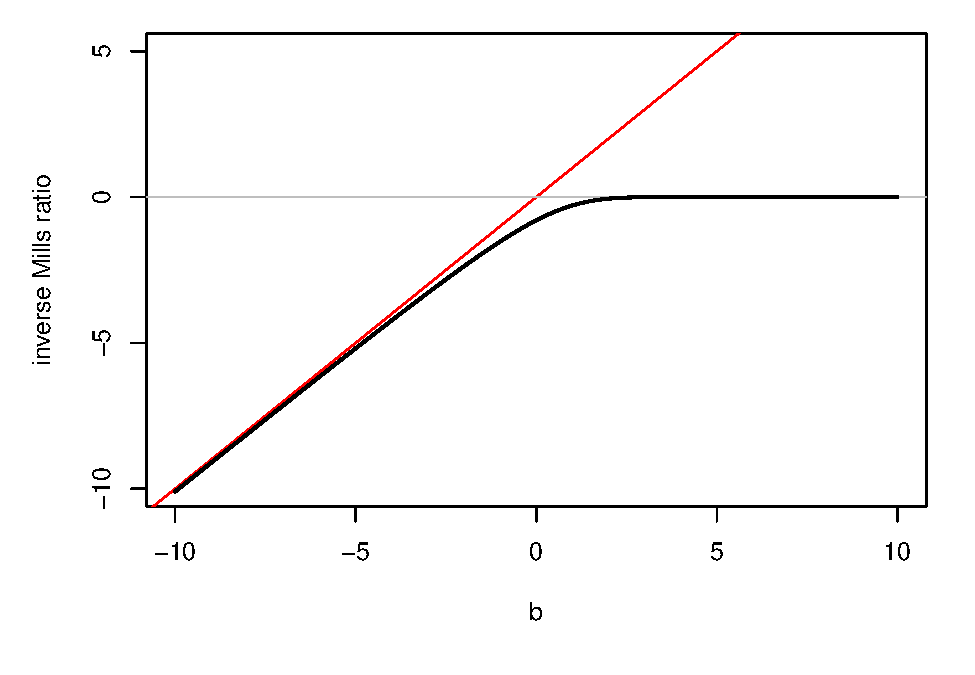
\includegraphics{AdvECTS_files/figure-latex/inverseMills-1} 

}

\caption{$\mathbb{E}(X|X<b)$ as a function of $b$ when $X\sim \mathcal{N}(0,1)$ (in black).}\label{fig:inverseMills}
\end{figure}

\begin{proposition}[p.d.f. of a multivariate Gaussian variable]
\protect\hypertarget{prp:pdfMultivarGaussian}{}\label{prp:pdfMultivarGaussian}If \(Y \sim \mathcal{N}(\mu,\Omega)\) and if \(Y\) is a \(n\)-dimensional vector, then the density function of \(Y\) is:
\[
\frac{1}{(2 \pi)^{n/2}|\Omega|^{1/2}}\exp\left[-\frac{1}{2}\left(Y-\mu\right)'\Omega^{-1}\left(Y-\mu\right)\right].
\]
\end{proposition}

\hypertarget{proofs}{%
\section{Proofs}\label{proofs}}

\hypertarget{MLEproperties}{%
\subsection{Proof of Proposition \ref{prp:MLEproperties}}\label{MLEproperties}}

\begin{proof}
Assumptions (i) and (ii) (in the set of Assumptions \ref{hyp:MLEregularity}) imply that \(\boldsymbol\theta_{MLE}\) exists (\(=\mbox{argmax}_\theta (1/n)\log \mathcal{L}(\boldsymbol\theta;\mathbf{y})\)).

\((1/n)\log \mathcal{L}(\boldsymbol\theta;\mathbf{y})\) can be interpreted as the sample mean of the r.v. \(\log f(Y_i;\boldsymbol\theta)\) that are i.i.d. Therefore \((1/n)\log \mathcal{L}(\boldsymbol\theta;\mathbf{y})\) converges to \(\mathbb{E}_{\boldsymbol\theta_0}(\log f(Y;\boldsymbol\theta))\) -- which exists (Assumption iv).

Because the latter convergence is uniform (Assumption v), the solution \(\boldsymbol\theta_{MLE}\) almost surely converges to the solution to the limit problem:
\[
\mbox{argmax}_\theta \mathbb{E}_{\boldsymbol\theta_0}(\log f(Y;\boldsymbol\theta)) = \mbox{argmax}_\theta \int_{\mathcal{Y}} \log f(y;\boldsymbol\theta)f(y;\boldsymbol\theta_0) dy.
\]

Properties of the Kullback information measure (see Prop. \ref{prp:Kullback}), together with the identifiability assumption (ii) implies that the solution to the limit problem is unique and equal to \(\boldsymbol\theta_0\).

Consider a r.v. sequence \(\boldsymbol\theta\) that converges to \(\boldsymbol\theta_0\). The Taylor expansion of the score in a neighborood of \(\boldsymbol\theta_0\) yields to:
\[
\frac{\partial \log \mathcal{L}(\boldsymbol\theta;\mathbf{y})}{\partial \boldsymbol\theta} = \frac{\partial \log \mathcal{L}(\boldsymbol\theta_0;\mathbf{y})}{\partial \boldsymbol\theta} + \frac{\partial^2 \log \mathcal{L}(\boldsymbol\theta_0;\mathbf{y})}{\partial \boldsymbol\theta \partial \boldsymbol\theta'}(\boldsymbol\theta - \boldsymbol\theta_0) + o_p(\boldsymbol\theta - \boldsymbol\theta_0)
\]

\(\boldsymbol\theta_{MLE}\) converges to \(\boldsymbol\theta_0\) and satisfies the likelihood equation \(\frac{\partial \log \mathcal{L}(\boldsymbol\theta;\mathbf{y})}{\partial \boldsymbol\theta} = \mathbf{0}\). Therefore:
\[
\frac{\partial \log \mathcal{L}(\boldsymbol\theta_0;\mathbf{y})}{\partial \boldsymbol\theta} \approx - \frac{\partial^2 \log \mathcal{L}(\boldsymbol\theta_0;\mathbf{y})}{\partial \boldsymbol\theta \partial \boldsymbol\theta'}(\boldsymbol\theta_{MLE} - \boldsymbol\theta_0),
\]
or equivalently:
\[
\frac{1}{\sqrt{n}} \frac{\partial \log \mathcal{L}(\boldsymbol\theta_0;\mathbf{y})}{\partial \boldsymbol\theta} \approx
\left(- \frac{1}{n} \sum_{i=1}^n \frac{\partial^2 \log f(y_i;\boldsymbol\theta_0)}{\partial \boldsymbol\theta \partial \boldsymbol\theta'} \right)\sqrt{n}(\boldsymbol\theta_{MLE} - \boldsymbol\theta_0),
\]

By the law of large numbers, we have: \(\left(- \frac{1}{n} \sum_{i=1}^n \frac{\partial^2 \log f(y_i;\boldsymbol\theta_0)}{\partial \boldsymbol\theta \partial \boldsymbol\theta'} \right) \overset{}\rightarrow \frac{1}{n} \mathbf{I}(\boldsymbol\theta_0) = \mathcal{I}_Y(\boldsymbol\theta_0)\).

Besides, we have:
\begin{eqnarray*}
\frac{1}{\sqrt{n}} \frac{\partial \log \mathcal{L}(\boldsymbol\theta_0;\mathbf{y})}{\partial \boldsymbol\theta} &=& \sqrt{n} \left( \frac{1}{n} \sum_i \frac{\partial \log f(y_i;\boldsymbol\theta_0)}{\partial \boldsymbol\theta} \right) \\
&=& \sqrt{n} \left( \frac{1}{n} \sum_i \left\{ \frac{\partial \log f(y_i;\boldsymbol\theta_0)}{\partial \boldsymbol\theta} - \mathbb{E}_{\boldsymbol\theta_0} \frac{\partial \log f(Y_i;\boldsymbol\theta_0)}{\partial \boldsymbol\theta} \right\} \right)
\end{eqnarray*}
which converges to \(\mathcal{N}(0,\mathcal{I}_Y(\boldsymbol\theta_0))\) by the CLT.

Collecting the preceding results leads to (b). The fact that \(\boldsymbol\theta_{MLE}\) achieves the FDCR bound proves (c).
\end{proof}

\hypertarget{Walddistri}{%
\subsection{Proof of Proposition \ref{prp:Walddistri}}\label{Walddistri}}

\begin{proof}
We have \(\sqrt{n}(\hat{\boldsymbol\theta}_{n} - \boldsymbol\theta_{0}) \overset{d}{\rightarrow} \mathcal{N}(0,\mathcal{I}(\boldsymbol\theta_0)^{-1})\) (Eq. \ref(eq:normMLE)). A Taylor expansion around \(\boldsymbol\theta_0\) yields to:
\begin{equation}
\sqrt{n}(h(\hat{\boldsymbol\theta}_{n}) - h(\boldsymbol\theta_{0})) \overset{d}{\rightarrow} \mathcal{N}\left(0,\frac{\partial h(\boldsymbol\theta_{0})}{\partial \boldsymbol\theta'}\mathcal{I}(\boldsymbol\theta_0)^{-1}\frac{\partial h(\boldsymbol\theta_{0})'}{\partial \boldsymbol\theta}\right). \label{eq:XXX}
\end{equation}
Under \(H_0\), \(h(\boldsymbol\theta_{0})=0\) therefore:
\begin{equation}
\sqrt{n} h(\hat{\boldsymbol\theta}_{n}) \overset{d}{\rightarrow} \mathcal{N}\left(0,\frac{\partial h(\boldsymbol\theta_{0})}{\partial \boldsymbol\theta'}\mathcal{I}(\boldsymbol\theta_0)^{-1}\frac{\partial h(\boldsymbol\theta_{0})'}{\partial \boldsymbol\theta}\right). \label{eq:lm10}
\end{equation}
Hence
\[
\sqrt{n} \left(
\frac{\partial h(\boldsymbol\theta_{0})}{\partial \boldsymbol\theta'}\mathcal{I}(\boldsymbol\theta_0)^{-1}\frac{\partial h(\boldsymbol\theta_{0})'}{\partial \boldsymbol\theta}
\right)^{-1/2} h(\hat{\boldsymbol\theta}_{n}) \overset{d}{\rightarrow} \mathcal{N}\left(0,Id\right).
\]
Taking the quadratic form, we obtain:
\[
n h(\hat{\boldsymbol\theta}_{n})'  \left(
\frac{\partial h(\boldsymbol\theta_{0})}{\partial \boldsymbol\theta'}\mathcal{I}(\boldsymbol\theta_0)^{-1}\frac{\partial h(\boldsymbol\theta_{0})'}{\partial \boldsymbol\theta}
\right)^{-1} h(\hat{\boldsymbol\theta}_{n}) \overset{d}{\rightarrow} \chi^2(r).
\]

The fact that the test has asymptotic level \(\alpha\) directly stems from what precedes. \textbf{Consistency of the test}: Consider \(\theta_0 \in \Theta\). Because the MLE is consistent, \(h(\hat{\boldsymbol\theta}_{n})\) converges to \(h(\boldsymbol\theta_0) \ne 0\). Eq. \eqref{eq:XXX} is still valid. It implies that \(\xi^W_n\) converges to \(+\infty\) and therefore that \(\mathbb{P}_{\boldsymbol\theta}(\xi^W_n \ge \chi^2_{1-\alpha}(r)) \rightarrow 1\).
\end{proof}

\hypertarget{LMdistri}{%
\subsection{Proof of Proposition \ref{prp:LMdistri}}\label{LMdistri}}

\begin{proof}
Notations: ``\(\approx\)'' means ``equal up to a term that converges to 0 in probability''. We are under \(H_0\). \(\hat{\boldsymbol\theta}^0\) is the constrained ML estimator; \(\hat{\boldsymbol\theta}\) denotes the unconstrained one.

We combine the two Taylor expansion: \(h(\hat{\boldsymbol\theta}_n) \approx \dfrac{\partial h(\boldsymbol\theta_0)}{\partial \boldsymbol\theta'}(\hat{\boldsymbol\theta}_n - \boldsymbol\theta_0)\) and \(h(\hat{\boldsymbol\theta}_n^0) \approx \dfrac{\partial h(\boldsymbol\theta_0)}{\partial \boldsymbol\theta'}(\hat{\boldsymbol\theta}_n^0 - \boldsymbol\theta_0)\) and we use \(h(\hat{\boldsymbol\theta}_n^0)=0\) (by definition) to get:
\begin{equation}
\sqrt{n}h(\hat{\boldsymbol\theta}_n) \approx \dfrac{\partial h(\boldsymbol\theta_0)}{\partial \boldsymbol\theta'}\sqrt{n}(\hat{\boldsymbol\theta}_n - \hat{\boldsymbol\theta}^0_n). \label{eq:lm1}
\end{equation}
Besides, we have (using the definition of the information matrix):
\begin{equation}
\frac{1}{\sqrt{n}}\frac{\partial \log \mathcal{L}(\hat{\boldsymbol\theta}^0_n;\mathbf{y})}{\partial \boldsymbol\theta} \approx
\frac{1}{\sqrt{n}}\frac{\partial \log \mathcal{L}(\boldsymbol\theta_0;\mathbf{y})}{\partial \boldsymbol\theta} - \mathcal{I}(\boldsymbol\theta_0)\sqrt{n}(\hat{\boldsymbol\theta}^0_n-\boldsymbol\theta_0) \label{eq:lm29}
\end{equation}
and:
\begin{equation}
0=\frac{1}{\sqrt{n}}\frac{\partial \log \mathcal{L}(\hat{\boldsymbol\theta}_n;\mathbf{y})}{\partial \boldsymbol\theta} \approx
\frac{1}{\sqrt{n}}\frac{\partial \log \mathcal{L}(\boldsymbol\theta_0;\mathbf{y})}{\partial \boldsymbol\theta} - \mathcal{I}(\boldsymbol\theta_0)\sqrt{n}(\hat{\boldsymbol\theta}_n-\boldsymbol\theta_0).\label{eq:lm30}
\end{equation}
Taking the difference and multiplying by \(\mathcal{I}(\boldsymbol\theta_0)^{-1}\):
\begin{equation}
\sqrt{n}(\hat{\boldsymbol\theta}_n-\hat{\boldsymbol\theta}_n^0) \approx
\mathcal{I}(\boldsymbol\theta_0)^{-1}\frac{1}{\sqrt{n}}\frac{\partial \log \mathcal{L}(\hat{\boldsymbol\theta}^0_n;\mathbf{y})}{\partial \boldsymbol\theta}
\mathcal{I}(\boldsymbol\theta_0).\label{eq:lm2}
\end{equation}
Eqs. \eqref{eq:lm1} and \eqref{eq:lm2} yield to:
\begin{equation}
\sqrt{n}h(\hat{\boldsymbol\theta}_n) \approx \dfrac{\partial h(\boldsymbol\theta_0)}{\partial \boldsymbol\theta'} \mathcal{I}(\boldsymbol\theta_0)^{-1}\frac{1}{\sqrt{n}}\frac{\partial \log \mathcal{L}(\hat{\boldsymbol\theta}^0_n;\mathbf{y})}{\partial \boldsymbol\theta}.\label{eq:lm3}
\end{equation}

Recall that \(\hat{\boldsymbol\theta}^0_n\) is the MLE of \(\boldsymbol\theta_0\) under the constraint \(h(\boldsymbol\theta)=0\). The vector of Lagrange multipliers \(\hat\lambda_n\) associated to this program satisfies:
\begin{equation}
\frac{\partial \log \mathcal{L}(\hat{\boldsymbol\theta}^0_n;\mathbf{y})}{\partial \boldsymbol\theta}+ \frac{\partial h'(\hat{\boldsymbol\theta}^0_n;\mathbf{y})}{\partial \boldsymbol\theta}\hat\lambda_n = 0.\label{eq:multiplier}
\end{equation}
Substituting the latter equation in Eq. \eqref{eq:lm3} gives:
\[
\sqrt{n}h(\hat{\boldsymbol\theta}_n) \approx
- \dfrac{\partial h(\boldsymbol\theta_0)}{\partial \boldsymbol\theta'} \mathcal{I}(\boldsymbol\theta_0)^{-1}
\frac{\partial h'(\hat{\boldsymbol\theta}^0_n;\mathbf{y})}{\partial \boldsymbol\theta} \frac{\hat\lambda_n}{\sqrt{n}} \approx
- \dfrac{\partial h(\boldsymbol\theta_0)}{\partial \boldsymbol\theta'} \mathcal{I}(\boldsymbol\theta_0)^{-1}
\frac{\partial h'(\boldsymbol\theta_0;\mathbf{y})}{\partial \boldsymbol\theta} \frac{\hat\lambda_n}{\sqrt{n}}
\]
which yields:
\begin{equation}
\frac{\hat\lambda_n}{\sqrt{n}} \approx - \left(
\dfrac{\partial h(\boldsymbol\theta_0)}{\partial \boldsymbol\theta'} \mathcal{I}(\boldsymbol\theta_0)^{-1}
\frac{\partial h'(\boldsymbol\theta_0;\mathbf{y})}{\partial \boldsymbol\theta}
\right)^{-1}
\sqrt{n}h(\hat{\boldsymbol\theta}_n).\label{eq:lm20}
\end{equation}
It follows, from Eq. \eqref{eq:lm10}, that:
\[
\frac{\hat\lambda_n}{\sqrt{n}} \overset{d}{\rightarrow} \mathcal{N}\left(0,\left(
\dfrac{\partial h(\boldsymbol\theta_0)}{\partial \boldsymbol\theta'} \mathcal{I}(\boldsymbol\theta_0)^{-1}
\frac{\partial h'(\boldsymbol\theta_0;\mathbf{y})}{\partial \boldsymbol\theta}
\right)^{-1}\right).
\]
Taking the quadratic form of the last equation gives:
\[
\frac{1}{n}\hat\lambda_n' \dfrac{\partial h(\hat{\boldsymbol\theta}^0_n)}{\partial \boldsymbol\theta'} \mathcal{I}(\hat{\boldsymbol\theta}^0_n)^{-1}
\frac{\partial h'(\hat{\boldsymbol\theta}^0_n;\mathbf{y})}{\partial \boldsymbol\theta} \hat\lambda_n \overset{d}{\rightarrow} \chi^2(r).
\]
Using Eq. \eqref{eq:multiplier}, it appears that the left-hand side term of the last equation is \(\xi^{LM}\) as defined in Eq. \eqref{eq:xiLM}. Consistency: see Remark 17.3 in \citet{gourieroux_monfort_1995}.
\end{proof}

\hypertarget{equivLRLMW}{%
\subsection{Proof of Proposition \ref{prp:equivLRLMW}}\label{equivLRLMW}}

\begin{proof}
Let us first demonstrate the asymptotic equivalence of \(\xi^{LM}\) and \(\xi^{LR}\).

The second-order taylor expansions of \(\log \mathcal{L}(\hat{\boldsymbol\theta}^0_n,\mathbf{y})\) and \(\log \mathcal{L}(\hat{\boldsymbol\theta}_n,\mathbf{y})\) are:
\begin{eqnarray*}
\log \mathcal{L}(\hat{\boldsymbol\theta}_n,\mathbf{y}) &\approx& \log \mathcal{L}(\boldsymbol\theta_0,\mathbf{y})
+ \frac{\partial \log \mathcal{L}(\boldsymbol\theta_0,\mathbf{y})}{\partial \boldsymbol\theta'}(\hat{\boldsymbol\theta}_n-\boldsymbol\theta_0)
- \frac{n}{2} (\hat{\boldsymbol\theta}_n-\boldsymbol\theta_0)' \mathcal{I}(\boldsymbol\theta_0) (\hat{\boldsymbol\theta}_n-\boldsymbol\theta_0)\\
\log \mathcal{L}(\hat{\boldsymbol\theta}^0_n,\mathbf{y}) &\approx& \log \mathcal{L}(\boldsymbol\theta_0,\mathbf{y})
+ \frac{\partial \log \mathcal{L}(\boldsymbol\theta_0,\mathbf{y})}{\partial \boldsymbol\theta'}(\hat{\boldsymbol\theta}^0_n-\boldsymbol\theta_0)
- \frac{n}{2} (\hat{\boldsymbol\theta}^0_n-\boldsymbol\theta_0)' \mathcal{I}(\boldsymbol\theta_0) (\hat{\boldsymbol\theta}^0_n-\boldsymbol\theta_0).
\end{eqnarray*}
Taking the difference, we obtain:
\[
\xi_n^{LR} \approx 2\frac{\partial \log \mathcal{L}(\boldsymbol\theta_0,\mathbf{y})}{\partial \boldsymbol\theta'}
(\hat{\boldsymbol\theta}_n-\hat{\boldsymbol\theta}^0_n) + n (\hat{\boldsymbol\theta}^0_n-\boldsymbol\theta_0)' \mathcal{I}(\boldsymbol\theta_0) (\hat{\boldsymbol\theta}^0_n-\boldsymbol\theta_0) - n (\hat{\boldsymbol\theta}_n-\boldsymbol\theta_0)' \mathcal{I}(\boldsymbol\theta_0) (\hat{\boldsymbol\theta}_n-\boldsymbol\theta_0).
\]
Using \(\dfrac{1}{\sqrt{n}}\frac{\partial \log \mathcal{L}(\boldsymbol\theta_0;\mathbf{y})}{\partial \boldsymbol\theta} \approx \mathcal{I}(\boldsymbol\theta_0)\sqrt{n}(\hat{\boldsymbol\theta}_n-\boldsymbol\theta_0)\) (Eq. \eqref{eq:lm30}), we have:
\[
\xi_n^{LR} \approx
2n(\hat{\boldsymbol\theta}_n-\boldsymbol\theta_0)'\mathcal{I}(\boldsymbol\theta_0)
(\hat{\boldsymbol\theta}_n-\hat{\boldsymbol\theta}^0_n)
+ n (\hat{\boldsymbol\theta}^0_n-\boldsymbol\theta_0)' \mathcal{I}(\boldsymbol\theta_0) (\hat{\boldsymbol\theta}^0_n-\boldsymbol\theta_0) - n (\hat{\boldsymbol\theta}_n-\boldsymbol\theta_0)' \mathcal{I}(\boldsymbol\theta_0) (\hat{\boldsymbol\theta}_n-\boldsymbol\theta_0).
\]
In the second of the three terms in the sum, we replace \((\hat{\boldsymbol\theta}^0_n-\boldsymbol\theta_0)\) by \((\hat{\boldsymbol\theta}^0_n-\hat{\boldsymbol\theta}_n+\hat{\boldsymbol\theta}_n-\boldsymbol\theta_0)\) and we develop the associated product. This leads to:
\begin{equation}
\xi_n^{LR} \approx n (\hat{\boldsymbol\theta}^0_n-\hat{\boldsymbol\theta}_n)' \mathcal{I}(\boldsymbol\theta_0)^{-1} (\hat{\boldsymbol\theta}^0_n-\hat{\boldsymbol\theta}_n). \label{eq:lr10}
\end{equation}
The difference between Eqs. \eqref{eq:lm29} and \eqref{eq:lm30} implies:
\[
\frac{1}{\sqrt{n}}\frac{\partial \log \mathcal{L}(\hat{\boldsymbol\theta}^0_n;\mathbf{y})}{\partial \boldsymbol\theta} \approx
\mathcal{I}(\boldsymbol\theta_0)\sqrt{n}(\hat{\boldsymbol\theta}_n-\hat{\boldsymbol\theta}^0_n),
\]
which, associated to Eq. @\ref(eq:lr10), gives:
\[
\xi_n^{LR} \approx \frac{1}{n} \frac{\partial \log \mathcal{L}(\hat{\boldsymbol\theta}^0_n;\mathbf{y})}{\partial \boldsymbol\theta'} \mathcal{I}(\boldsymbol\theta_0)^{-1} \frac{\partial \log \mathcal{L}(\hat{\boldsymbol\theta}^0_n;\mathbf{y})}{\partial \boldsymbol\theta} \approx \xi_n^{LM}.
\]
Hence \(\xi_n^{LR}\) has the same asymptotic distribution as \(\xi_n^{LM}\).

Let's show that the LR test is consistent. For this, note that:
\[
\frac{\log \mathcal{L}(\hat{\boldsymbol\theta},\mathbf{y}) - \log \mathcal{L}(\hat{\boldsymbol\theta}^0,\mathbf{y})}{n} = \frac{1}{n} \sum_{i=1}^n[\log f(y_i;\hat{\boldsymbol\theta}_n) - \log f(y_i;\hat{\boldsymbol\theta}_n^0)] \rightarrow \mathbb{E}_0[\log f(Y;\boldsymbol\theta_0) - \log f(Y;\boldsymbol\theta_\infty)],
\]
where \(\boldsymbol\theta_\infty\), the pseudo true value, is such that \(h(\boldsymbol\theta_\infty) \ne 0\) (by definition of \(H_1\)). From the Kullback inequality and the asymptotic identifiability of \(\boldsymbol\theta_0\), it follows that \(\mathbb{E}_0[\log f(Y;\boldsymbol\theta_0) - \log f(Y;\boldsymbol\theta_\infty)] >0\). Therefore \(\xi_n^{LR} \rightarrow + \infty\) under \(H_1\).

Let us now demonstrate the equivalence of \(\xi^{LM} and \xi^{W}\).

We have (using Eq. \ref(eq:multiplier)):
\[
\xi^{LM}_n = \frac{1}{n}\hat\lambda_n' \dfrac{\partial h(\hat{\boldsymbol\theta}^0_n)}{\partial \boldsymbol\theta'} \mathcal{I}(\hat{\boldsymbol\theta}^0_n)^{-1}
\frac{\partial h'(\hat{\boldsymbol\theta}^0_n;\mathbf{y})}{\partial \boldsymbol\theta} \hat\lambda_n.
\]
Since, under \(H_0\), \(\hat{\boldsymbol\theta}_n^0\approx\hat{\boldsymbol\theta}_n \approx {\boldsymbol\theta}_0\), Eq. \eqref{eq:lm20} therefore implies that:
\[
\xi^{LM} \approx n h(\hat{\boldsymbol\theta}_n)' \left(
\dfrac{\partial h(\hat{\boldsymbol\theta}_n)}{\partial \boldsymbol\theta'} \mathcal{I}(\hat{\boldsymbol\theta}_n)^{-1}
\frac{\partial h'(\hat{\boldsymbol\theta}_n;\mathbf{y})}{\partial \boldsymbol\theta}
\right)^{-1}
h(\hat{\boldsymbol\theta}_n) = \xi^{W},
\]
which gives the result.
\end{proof}

\hypertarget{proofTVTCL}{%
\subsection{Proof of Eq. \eqref{eq:TCL2}}\label{proofTVTCL}}

\begin{proof}
We have:
\begin{eqnarray*}
&&T\mathbb{E}\left[(\bar{y}_T - \mu)^2\right]\\
&=& T\mathbb{E}\left[\left(\frac{1}{T}\sum_{t=1}^T(y_t - \mu)\right)^2\right] = \frac{1}{T} \mathbb{E}\left[\sum_{t=1}^T(y_t - \mu)^2+2\sum_{s<t\le T}(y_t - \mu)(y_s - \mu)\right]\\
&=& \gamma_0 +\frac{2}{T}\left(\sum_{t=2}^{T}\mathbb{E}\left[(y_t - \mu)(y_{t-1} - \mu)\right]\right) +\frac{2}{T}\left(\sum_{t=3}^{T}\mathbb{E}\left[(y_t - \mu)(y_{t-2} - \mu)\right]\right) + \dots \\
&&+ \frac{2}{T}\left(\sum_{t=T-1}^{T}\mathbb{E}\left[(y_t - \mu)(y_{t-(T-2)} - \mu)\right]\right) + \frac{2}{T}\mathbb{E}\left[(y_t - \mu)(y_{t-(T-1)} - \mu)\right]\\
&=&  \gamma_0 + 2 \frac{T-1}{T}\gamma_1 + \dots + 2 \frac{1}{T}\gamma_{T-1} .
\end{eqnarray*}
Therefore:
\begin{eqnarray*}
T\mathbb{E}\left[(\bar{y}_T - \mu)^2\right] - \sum_{j=-\infty}^{+\infty} \gamma_j &=& - 2\frac{1}{T}\gamma_1 - 2\frac{2}{T}\gamma_2 - \dots - 2\frac{T-1}{T}\gamma_{T-1} - 2\gamma_T - 2 \gamma_{T+1} + \dots
\end{eqnarray*}
And then:
\[
\left|T\mathbb{E}\left[(\bar{y}_T - \mu)^2\right] - \sum_{j=-\infty}^{+\infty} \gamma_j\right| \le 2\frac{1}{T}|\gamma_1| + 2\frac{2}{T}|\gamma_2| + \dots + 2\frac{T-1}{T}|\gamma_{T-1}| + 2|\gamma_T| + 2 |\gamma_{T+1}| + \dots
\]

For any \(q \le T\), we have:
\begin{eqnarray*}
\left|T\mathbb{E}\left[(\bar{y}_T - \mu)^2\right] - \sum_{j=-\infty}^{+\infty} \gamma_j\right| &\le& 2\frac{1}{T}|\gamma_1| + 2\frac{2}{T}|\gamma_2| + \dots + 2\frac{q-1}{T}|\gamma_{q-1}| +2\frac{q}{T}|\gamma_q| +\\
&&2\frac{q+1}{T}|\gamma_{q+1}| + \dots  + 2\frac{T-1}{T}|\gamma_{T-1}| + 2|\gamma_T| + 2 |\gamma_{T+1}| + \dots\\
&\le& \frac{2}{T}\left(|\gamma_1| + 2|\gamma_2| + \dots + (q-1)|\gamma_{q-1}| +q|\gamma_q|\right) +\\
&&2|\gamma_{q+1}| + \dots  + 2|\gamma_{T-1}| + 2|\gamma_T| + 2 |\gamma_{T+1}| + \dots
\end{eqnarray*}

Consider \(\varepsilon > 0\). The fact that the autocovariances are absolutely summable implies that there exists \(q_0\) such that (Cauchy criterion, Theorem \ref{thm:cauchycritstatic}):
\[
2|\gamma_{q_0+1}|+2|\gamma_{q_0+2}|+2|\gamma_{q_0+3}|+\dots < \varepsilon/2.
\]
Then, if \(T > q_0\), it comes that:
\[
\left|T \mathbb{E}\left[(\bar{y}_T - \mu)^2\right] - \sum_{j=-\infty}^{+\infty} \gamma_j\right|\le \frac{2}{T}\left(|\gamma_1| + 2|\gamma_2| + \dots + (q_0-1)|\gamma_{q_0-1}| +q_0|\gamma_{q_0}|\right) + \varepsilon/2.
\]
If \(T \ge 2\left(|\gamma_1| + 2|\gamma_2| + \dots + (q_0-1)|\gamma_{q_0-1}| +q_0|\gamma_{q_0}|\right)/(\varepsilon/2)\) (\(= f(q_0)\), say) then
\[
\frac{2}{T}\left(|\gamma_1| + 2|\gamma_2| + \dots + (q_0-1)|\gamma_{q_0-1}| +q_0|\gamma_{q_0}|\right) \le \varepsilon/2.
\]
Then, if \(T>f(q_0)\) and \(T>q_0\), i.e.~if \(T>\max(f(q_0),q_0)\), we have:
\[
\left|T \mathbb{E}\left[(\bar{y}_T - \mu)^2\right] - \sum_{j=-\infty}^{+\infty} \gamma_j\right|\le \varepsilon.
\]
\end{proof}

\hypertarget{smallestMSE}{%
\subsection{Proof of Proposition \ref{prp:smallestMSE}}\label{smallestMSE}}

\begin{proof}
We have:
\begin{eqnarray}
\mathbb{E}([y_{t+1} - y^*_{t+1}]^2) &=& \mathbb{E}\left([\color{blue}{\{y_{t+1} - \mathbb{E}(y_{t+1}|x_t)\}} + \color{red}{\{\mathbb{E}(y_{t+1}|x_t)  - y^*_{t+1}\}}]^2\right)\nonumber\\
&=&  \mathbb{E}\left(\color{blue}{[y_{t+1} - \mathbb{E}(y_{t+1}|x_t)]}^2\right) + \mathbb{E}\left(\color{red}{[\mathbb{E}(y_{t+1}|x_t)  - y^*_{t+1}]}^2\right)\nonumber\\
&& + 2\mathbb{E}\left( \color{blue}{[y_{t+1} - \mathbb{E}(y_{t+1}|x_t)]}\color{red}{ [\mathbb{E}(y_{t+1}|x_t)  - y^*_{t+1}]}\right). \label{eq:1}
\end{eqnarray}
Let us focus on the last term. We have:
\begin{eqnarray*}
&&\mathbb{E}\left(\color{blue}{[y_{t+1} - \mathbb{E}(y_{t+1}|x_t)]}\color{red}{ [\mathbb{E}(y_{t+1}|x_t)  - y^*_{t+1}]}\right)\\
&=& \mathbb{E}( \mathbb{E}( \color{blue}{[y_{t+1} - \mathbb{E}(y_{t+1}|x_t)]}\color{red}{ \underbrace{[\mathbb{E}(y_{t+1}|x_t)  - y^*_{t+1}]}_{\mbox{function of $x_t$}}}|x_t))\\
&=& \mathbb{E}( \color{red}{ [\mathbb{E}(y_{t+1}|x_t)  - y^*_{t+1}]} \mathbb{E}( \color{blue}{[y_{t+1} - \mathbb{E}(y_{t+1}|x_t)]}|x_t))\\
&=& \mathbb{E}( \color{red}{ [\mathbb{E}(y_{t+1}|x_t)  - y^*_{t+1}]} \color{blue}{\underbrace{[\mathbb{E}(y_{t+1}|x_t) - \mathbb{E}(y_{t+1}|x_t)]}_{=0}})=0.
\end{eqnarray*}

Therefore, Eq. \eqref{eq:1} becomes:
\begin{eqnarray*}
&&\mathbb{E}([y_{t+1} - y^*_{t+1}]^2) \\
&=&  \underbrace{\mathbb{E}\left(\color{blue}{[y_{t+1} - \mathbb{E}(y_{t+1}|x_t)]}^2\right)}_{\mbox{$\ge 0$ and does not depend on $y^*_{t+1}$}} + \underbrace{\mathbb{E}\left(\color{red}{[\mathbb{E}(y_{t+1}|x_t)  - y^*_{t+1}]}^2\right)}_{\mbox{$\ge 0$ and depends on $y^*_{t+1}$}}.
\end{eqnarray*}
This implies that \(\mathbb{E}([y_{t+1} - y^*_{t+1}]^2)\) is always larger than \(\color{blue}{\mathbb{E}([y_{t+1} - \mathbb{E}(y_{t+1}|x_t)]^2)}\), and is therefore minimized if the second term is equal to zero, that is if \(\mathbb{E}(y_{t+1}|x_t) = y^*_{t+1}\).
\end{proof}

\hypertarget{estimVARGaussian}{%
\subsection{Proof of Proposition \ref{prp:estimVARGaussian}}\label{estimVARGaussian}}

\begin{proof}
Using Proposition \ref{prp:multivarG} (in Appendix \ref{XXX}), we obtain that, conditionally on \(x_1\), the log-likelihood is given by
\begin{eqnarray*}
\log\mathcal{L}(Y_{T};\theta) & = & -(Tn/2)\log(2\pi)+(T/2)\log\left|\Omega^{-1}\right|\\
&  & -\frac{1}{2}\sum_{t=1}^{T}\left[\left(y_{t}-\Pi'x_{t}\right)'\Omega^{-1}\left(y_{t}-\Pi'x_{t}\right)\right].
\end{eqnarray*}
Let's rewrite the last term of the log-likelihood:
\begin{eqnarray*}
\sum_{t=1}^{T}\left[\left(y_{t}-\Pi'x_{t}\right)'\Omega^{-1}\left(y_{t}-\Pi'x_{t}\right)\right] & =\\
\sum_{t=1}^{T}\left[\left(y_{t}-\hat{\Pi}'x_{t}+\hat{\Pi}'x_{t}-\Pi'x_{t}\right)'\Omega^{-1}\left(y_{t}-\hat{\Pi}'x_{t}+\hat{\Pi}'x_{t}-\Pi'x_{t}\right)\right] & =\\
\sum_{t=1}^{T}\left[\left(\hat{\varepsilon}_{t}+(\hat{\Pi}-\Pi)'x_{t}\right)'\Omega^{-1}\left(\hat{\varepsilon}_{t}+(\hat{\Pi}-\Pi)'x_{t}\right)\right],
\end{eqnarray*}
where the \(j^{th}\) element of the \((n\times1)\) vector \(\hat{\varepsilon}_{t}\) is the sample residual, for observation \(t\), from an OLS regression of \(y_{j,t}\) on \(x_{t}\). Expanding the previous equation, we get:
\begin{eqnarray*}
&&\sum_{t=1}^{T}\left[\left(y_{t}-\Pi'x_{t}\right)'\Omega^{-1}\left(y_{t}-\Pi'x_{t}\right)\right]  = \sum_{t=1}^{T}\hat{\varepsilon}_{t}'\Omega^{-1}\hat{\varepsilon}_{t}\\
&&+2\sum_{t=1}^{T}\hat{\varepsilon}_{t}'\Omega^{-1}(\hat{\Pi}-\Pi)'x_{t}+\sum_{t=1}^{T}x'_{t}(\hat{\Pi}-\Pi)\Omega^{-1}(\hat{\Pi}-\Pi)'x_{t}.
\end{eqnarray*}
Let's apply the trace operator on the second term (that is a scalar):
\begin{eqnarray*}
\sum_{t=1}^{T}\hat{\varepsilon}_{t}'\Omega^{-1}(\hat{\Pi}-\Pi)'x_{t} & = & Tr\left(\sum_{t=1}^{T}\hat{\varepsilon}_{t}'\Omega^{-1}(\hat{\Pi}-\Pi)'x_{t}\right)\\
=  Tr\left(\sum_{t=1}^{T}\Omega^{-1}(\hat{\Pi}-\Pi)'x_{t}\hat{\varepsilon}_{t}'\right) & = & Tr\left(\Omega^{-1}(\hat{\Pi}-\Pi)'\sum_{t=1}^{T}x_{t}\hat{\varepsilon}_{t}'\right).
\end{eqnarray*}
Given that, by construction (property of OLS estimates), the sample residuals are orthogonal to the explanatory variables, this term is zero. Introducing \(\tilde{x}_{t}=(\hat{\Pi}-\Pi)'x_{t}\), we have
\begin{eqnarray*}
\sum_{t=1}^{T}\left[\left(y_{t}-\Pi'x_{t}\right)'\Omega^{-1}\left(y_{t}-\Pi'x_{t}\right)\right] =\sum_{t=1}^{T}\hat{\varepsilon}_{t}'\Omega^{-1}\hat{\varepsilon}_{t}+\sum_{t=1}^{T}\tilde{x}'_{t}\Omega^{-1}\tilde{x}_{t}.
\end{eqnarray*}
Since \(\Omega\) is a positive definite matrix, \(\Omega^{-1}\) is as well. Consequently, the smallest value that the last term can take is obtained for \(\tilde{x}_{t}=0\), i.e.~when \(\Pi=\hat{\Pi}.\)

The MLE of \(\Omega\) is the matrix \(\hat{\Omega}\) that maximizes \(\Omega\overset{\ell}{\rightarrow}L(Y_{T};\hat{\Pi},\Omega)\). We have:
\begin{eqnarray*}
\log\mathcal{L}(Y_{T};\hat{\Pi},\Omega) & = & -(Tn/2)\log(2\pi)+(T/2)\log\left|\Omega^{-1}\right| -\frac{1}{2}\sum_{t=1}^{T}\left[\hat{\varepsilon}_{t}'\Omega^{-1}\hat{\varepsilon}_{t}\right].
\end{eqnarray*}

Matrix \(\hat{\Omega}\) is a symmetric positive definite. It is easily checked that the (unrestricted) matrix that maximizes the latter expression is symmetric positive definite matrix. Indeed:
\[
\frac{\partial \log\mathcal{L}(Y_{T};\hat{\Pi},\Omega)}{\partial\Omega}=\frac{T}{2}\Omega'-\frac{1}{2}\sum_{t=1}^{T}\hat{\varepsilon}_{t}\hat{\varepsilon}'_{t}\Rightarrow\hat{\Omega}'=\frac{1}{T}\sum_{t=1}^{T}\hat{\varepsilon}_{t}\hat{\varepsilon}'_{t},
\]
which leads to the result.
\end{proof}

\hypertarget{OLSVAR}{%
\subsection{Proof of Proposition \ref{prp:OLSVAR}}\label{OLSVAR}}

\begin{proof}
Let us drop the \(i\) subscript. Rearranging Eq. \eqref{eq:olsar1}, we have:
\[
\sqrt{T}(\mathbf{b}-\boldsymbol{\beta}) =  (X'X/T)^{-1}\sqrt{T}(X'\boldsymbol\varepsilon/T).
\]
Let us consider the autocovariances of \(\mathbf{v}_t = x_t \varepsilon_t\), denoted by \(\gamma^v_j\). Using the fact that \(x_t\) is a linear combination of past \(\varepsilon_t\)s and that \(\varepsilon_t\) is a white noise, we get that \(\mathbb{E}(\varepsilon_t x_t)=0\). Therefore
\[
\gamma^v_j = \mathbb{E}(\varepsilon_t\varepsilon_{t-j}x_tx_{t-j}').
\]
If \(j>0\), we have \(\mathbb{E}(\varepsilon_t\varepsilon_{t-j}x_tx_{t-j}')=\mathbb{E}(\mathbb{E}[\varepsilon_t\varepsilon_{t-j}x_tx_{t-j}'|\varepsilon_{t-j},x_t,x_{t-j}])=\) \(\mathbb{E}(\varepsilon_{t-j}x_tx_{t-j}'\mathbb{E}[\varepsilon_t|\varepsilon_{t-j},x_t,x_{t-j}])=0\). Note that we have \(\mathbb{E}[\varepsilon_t|\varepsilon_{t-j},x_t,x_{t-j}]=0\) because \(\{\varepsilon_t\}\) is an i.i.d. white noise sequence. If \(j=0\), we have:
\[
\gamma^v_0 = \mathbb{E}(\varepsilon_t^2x_tx_{t}')= \mathbb{E}(\varepsilon_t^2) \mathbb{E}(x_tx_{t}')=\sigma^2\mathbf{Q}.
\]
The convergence in distribution of \(\sqrt{T}(X'\boldsymbol\varepsilon/T)=\sqrt{T}\frac{1}{T}\sum_{t=1}^Tv_t\) results from the Central Limit Theorem for covariance-stationary processes, using the \(\gamma_j^v\) computed above.
\end{proof}

\hypertarget{additional-codes}{%
\section{Additional codes}\label{additional-codes}}

\hypertarget{App:GEV}{%
\subsection{Simulating GEV distributions}\label{App:GEV}}

The following lines of code have been used to generate Figure \ref{fig:GEV}.

\begin{Shaded}
\begin{Highlighting}[]
\NormalTok{n.sim }\OtherTok{\textless{}{-}} \DecValTok{4000}
\FunctionTok{par}\NormalTok{(}\AttributeTok{mfrow=}\FunctionTok{c}\NormalTok{(}\DecValTok{1}\NormalTok{,}\DecValTok{3}\NormalTok{),}
    \AttributeTok{plt=}\FunctionTok{c}\NormalTok{(.}\DecValTok{2}\NormalTok{,.}\DecValTok{95}\NormalTok{,.}\DecValTok{2}\NormalTok{,.}\DecValTok{85}\NormalTok{))}
\NormalTok{all.rhos }\OtherTok{\textless{}{-}} \FunctionTok{c}\NormalTok{(.}\DecValTok{3}\NormalTok{,.}\DecValTok{6}\NormalTok{,.}\DecValTok{95}\NormalTok{)}
\ControlFlowTok{for}\NormalTok{(j }\ControlFlowTok{in} \DecValTok{1}\SpecialCharTok{:}\FunctionTok{length}\NormalTok{(all.rhos))\{}
\NormalTok{  theta }\OtherTok{\textless{}{-}} \DecValTok{1}\SpecialCharTok{/}\NormalTok{all.rhos[j]}
\NormalTok{  v1 }\OtherTok{\textless{}{-}} \FunctionTok{runif}\NormalTok{(n.sim)}
\NormalTok{  v2 }\OtherTok{\textless{}{-}} \FunctionTok{runif}\NormalTok{(n.sim)}
\NormalTok{  w }\OtherTok{\textless{}{-}} \FunctionTok{rep}\NormalTok{(.}\DecValTok{000001}\NormalTok{,n.sim)}
  \CommentTok{\# solve for f(w) = w*(1 {-} log(w)/theta) {-} v2 = 0}
  \ControlFlowTok{for}\NormalTok{(i }\ControlFlowTok{in} \DecValTok{1}\SpecialCharTok{:}\DecValTok{20}\NormalTok{)\{}
\NormalTok{    f.i }\OtherTok{\textless{}{-}}\NormalTok{ w }\SpecialCharTok{*}\NormalTok{ (}\DecValTok{1} \SpecialCharTok{{-}} \FunctionTok{log}\NormalTok{(w)}\SpecialCharTok{/}\NormalTok{theta) }\SpecialCharTok{{-}}\NormalTok{ v2}
\NormalTok{    f.prime }\OtherTok{\textless{}{-}} \DecValTok{1} \SpecialCharTok{{-}} \FunctionTok{log}\NormalTok{(w)}\SpecialCharTok{/}\NormalTok{theta }\SpecialCharTok{{-}} \DecValTok{1}\SpecialCharTok{/}\NormalTok{theta}
\NormalTok{    w }\OtherTok{\textless{}{-}}\NormalTok{ w }\SpecialCharTok{{-}}\NormalTok{ f.i}\SpecialCharTok{/}\NormalTok{f.prime}
\NormalTok{  \}}
\NormalTok{  u1 }\OtherTok{\textless{}{-}} \FunctionTok{exp}\NormalTok{(v1}\SpecialCharTok{\^{}}\NormalTok{(}\DecValTok{1}\SpecialCharTok{/}\NormalTok{theta) }\SpecialCharTok{*} \FunctionTok{log}\NormalTok{(w))}
\NormalTok{  u2 }\OtherTok{\textless{}{-}} \FunctionTok{exp}\NormalTok{((}\DecValTok{1}\SpecialCharTok{{-}}\NormalTok{v1)}\SpecialCharTok{\^{}}\NormalTok{(}\DecValTok{1}\SpecialCharTok{/}\NormalTok{theta) }\SpecialCharTok{*} \FunctionTok{log}\NormalTok{(w))}

  \CommentTok{\# Get eps1 and eps2 using the inverse of the Gumbel distribution\textquotesingle{}s cdf:}
\NormalTok{  eps1 }\OtherTok{\textless{}{-}} \SpecialCharTok{{-}}\FunctionTok{log}\NormalTok{(}\SpecialCharTok{{-}}\FunctionTok{log}\NormalTok{(u1))}
\NormalTok{  eps2 }\OtherTok{\textless{}{-}} \SpecialCharTok{{-}}\FunctionTok{log}\NormalTok{(}\SpecialCharTok{{-}}\FunctionTok{log}\NormalTok{(u2))}
  \FunctionTok{cbind}\NormalTok{(}\FunctionTok{cor}\NormalTok{(eps1,eps2),}\DecValTok{1}\SpecialCharTok{{-}}\NormalTok{all.rhos[j]}\SpecialCharTok{\^{}}\DecValTok{2}\NormalTok{)}
  \FunctionTok{plot}\NormalTok{(eps1,eps2,}\AttributeTok{pch=}\DecValTok{19}\NormalTok{,}\AttributeTok{col=}\StringTok{"\#FF000044"}\NormalTok{,}
       \AttributeTok{main=}\FunctionTok{paste}\NormalTok{(}\StringTok{"rho = "}\NormalTok{,}\FunctionTok{toString}\NormalTok{(all.rhos[j]),}\AttributeTok{sep=}\StringTok{""}\NormalTok{),}
       \AttributeTok{xlab=}\FunctionTok{expression}\NormalTok{(epsilon[}\DecValTok{1}\NormalTok{]),}
       \AttributeTok{ylab=}\FunctionTok{expression}\NormalTok{(epsilon[}\DecValTok{2}\NormalTok{]),}
       \AttributeTok{cex.lab=}\DecValTok{2}\NormalTok{,}\AttributeTok{cex.main=}\FloatTok{1.5}\NormalTok{)}
\NormalTok{\}}
\end{Highlighting}
\end{Shaded}

\hypertarget{IRFDELTA}{%
\subsection{Computing the covariance matrix of IRF using the delta method}\label{IRFDELTA}}

\begin{Shaded}
\begin{Highlighting}[]
\NormalTok{irf.function }\OtherTok{\textless{}{-}} \ControlFlowTok{function}\NormalTok{(THETA)\{}
\NormalTok{  c }\OtherTok{\textless{}{-}}\NormalTok{ THETA[}\DecValTok{1}\NormalTok{]}
\NormalTok{  phi }\OtherTok{\textless{}{-}}\NormalTok{ THETA[}\DecValTok{2}\SpecialCharTok{:}\NormalTok{(p}\SpecialCharTok{+}\DecValTok{1}\NormalTok{)]}
  \ControlFlowTok{if}\NormalTok{(q}\SpecialCharTok{\textgreater{}}\DecValTok{0}\NormalTok{)\{}
\NormalTok{    theta }\OtherTok{\textless{}{-}} \FunctionTok{c}\NormalTok{(}\DecValTok{1}\NormalTok{,THETA[(}\DecValTok{1}\SpecialCharTok{+}\NormalTok{p}\SpecialCharTok{+}\DecValTok{1}\NormalTok{)}\SpecialCharTok{:}\NormalTok{(}\DecValTok{1}\SpecialCharTok{+}\NormalTok{p}\SpecialCharTok{+}\NormalTok{q)])}
\NormalTok{  \}}\ControlFlowTok{else}\NormalTok{\{}
\NormalTok{    theta }\OtherTok{\textless{}{-}} \DecValTok{1}
\NormalTok{  \}}
\NormalTok{  sigma }\OtherTok{\textless{}{-}}\NormalTok{ THETA[}\DecValTok{1}\SpecialCharTok{+}\NormalTok{p}\SpecialCharTok{+}\NormalTok{q}\SpecialCharTok{+}\DecValTok{1}\NormalTok{]}
\NormalTok{  r }\OtherTok{\textless{}{-}} \FunctionTok{dim}\NormalTok{(Matrix.of.Exog)[}\DecValTok{2}\NormalTok{] }\SpecialCharTok{{-}} \DecValTok{1}
\NormalTok{  beta }\OtherTok{\textless{}{-}}\NormalTok{ THETA[(}\DecValTok{1}\SpecialCharTok{+}\NormalTok{p}\SpecialCharTok{+}\NormalTok{q}\SpecialCharTok{+}\DecValTok{1}\SpecialCharTok{+}\DecValTok{1}\NormalTok{)}\SpecialCharTok{:}\NormalTok{(}\DecValTok{1}\SpecialCharTok{+}\NormalTok{p}\SpecialCharTok{+}\NormalTok{q}\SpecialCharTok{+}\DecValTok{1}\SpecialCharTok{+}\NormalTok{(r}\SpecialCharTok{+}\DecValTok{1}\NormalTok{))]}
  
\NormalTok{  irf }\OtherTok{\textless{}{-}} \FunctionTok{sim.arma}\NormalTok{(}\DecValTok{0}\NormalTok{,phi,beta,}\AttributeTok{sigma=}\FunctionTok{sd}\NormalTok{(Ramey}\SpecialCharTok{$}\NormalTok{ED3\_TC,}\AttributeTok{na.rm=}\ConstantTok{TRUE}\NormalTok{),}\AttributeTok{T=}\DecValTok{60}\NormalTok{,}\AttributeTok{y.0=}\FunctionTok{rep}\NormalTok{(}\DecValTok{0}\NormalTok{,}\FunctionTok{length}\NormalTok{(x}\SpecialCharTok{$}\NormalTok{phi)),}\AttributeTok{nb.sim=}\DecValTok{1}\NormalTok{,}\AttributeTok{make.IRF=}\DecValTok{1}\NormalTok{,}
                  \AttributeTok{X=}\ConstantTok{NaN}\NormalTok{,}\AttributeTok{beta=}\ConstantTok{NaN}\NormalTok{)}
  \FunctionTok{return}\NormalTok{(irf)}
\NormalTok{\}}

\NormalTok{IRF}\FloatTok{.0} \OtherTok{\textless{}{-}} \DecValTok{100}\SpecialCharTok{*}\FunctionTok{irf.function}\NormalTok{(x}\SpecialCharTok{$}\NormalTok{THETA)}
\NormalTok{eps }\OtherTok{\textless{}{-}}\NormalTok{ .}\DecValTok{00000001}
\NormalTok{d.IRF }\OtherTok{\textless{}{-}} \ConstantTok{NULL}
\ControlFlowTok{for}\NormalTok{(i }\ControlFlowTok{in} \DecValTok{1}\SpecialCharTok{:}\FunctionTok{length}\NormalTok{(x}\SpecialCharTok{$}\NormalTok{THETA))\{}
\NormalTok{  THETA.i }\OtherTok{\textless{}{-}}\NormalTok{ x}\SpecialCharTok{$}\NormalTok{THETA}
\NormalTok{  THETA.i[i] }\OtherTok{\textless{}{-}}\NormalTok{ THETA.i[i] }\SpecialCharTok{+}\NormalTok{ eps}
\NormalTok{  IRF.i }\OtherTok{\textless{}{-}} \DecValTok{100}\SpecialCharTok{*}\FunctionTok{irf.function}\NormalTok{(THETA.i)}
\NormalTok{  d.IRF }\OtherTok{\textless{}{-}} \FunctionTok{cbind}\NormalTok{(d.IRF,}
\NormalTok{                 (IRF.i }\SpecialCharTok{{-}}\NormalTok{ IRF}\FloatTok{.0}\NormalTok{)}\SpecialCharTok{/}\NormalTok{eps}
\NormalTok{                 )}
\NormalTok{\}}
\NormalTok{mat.var.cov.IRF }\OtherTok{\textless{}{-}}\NormalTok{ d.IRF }\SpecialCharTok{\%*\%}\NormalTok{ x}\SpecialCharTok{$}\NormalTok{I }\SpecialCharTok{\%*\%} \FunctionTok{t}\NormalTok{(d.IRF)}
\end{Highlighting}
\end{Shaded}


  \bibliography{book.bib,packages.bib}

\end{document}
